%%%%%%%%%%%%%%%%%%%%%%%%%%%%%%%%%%%%%%%%%%%%%%%%%%%%%%%
\documentclass{article}
%%%%%%%%%%%%%%%%%%%%%%%%%%%%%%%%%%%%%%%%%%%%%%%%%%%%%%%
\usepackage[utf8]{vietnam}
%%%%%%%%%%%%%%%%%%%%%%%%%%%%%%%%%%%%%%%%%%%%%%%%%%%%%%%
\usepackage{graphicx}
%%%%%%%%%%%%%%%%%%%%%%%%%%%%%%%%%%%%%%%%%%%%%%%%%%%%%%%
\usepackage{hyperref}
%%%%%%%%%%%%%%%%%%%%%%%%%%%%%%%%%%%%%%%%%%%%%%%%%%%%%%%
\usepackage{xcolor}
\pagecolor[RGB]{40, 42, 54}% Đặt màu nền
\color[RGB]{18, 161, 24} % Đặt màu chữ
%%%%%%%%%%%%%%%%%%%%%%%%%%%%%%%%%%%%%%%%%%%%%%%%%%%%%%%
\usepackage{float} % Cố định hình ảnh [H]
%%%%%%%%%%%%%%%%%%%%%%%%%%%%%%%%%%%%%%%%%%%%%%%%%%%%%%%
\begin{document}
%%%%%%%%%%%%%%%%%%%%%%%%%%%%%%%%%%%%%%%%%%%%%%%%%%%%%%%
\listoffigures
\newpage
%%%%%%%%%%%%%%%%%%%%%%%%%%%%%%%%%%%%%%%%%%%%%%%%%%%%%%%
\section{Tuần 1: Thực hành tiền xử lý dữ liệu (ETL) cơ bản trong Excel}

\begin{figure}[h]
    \centering
    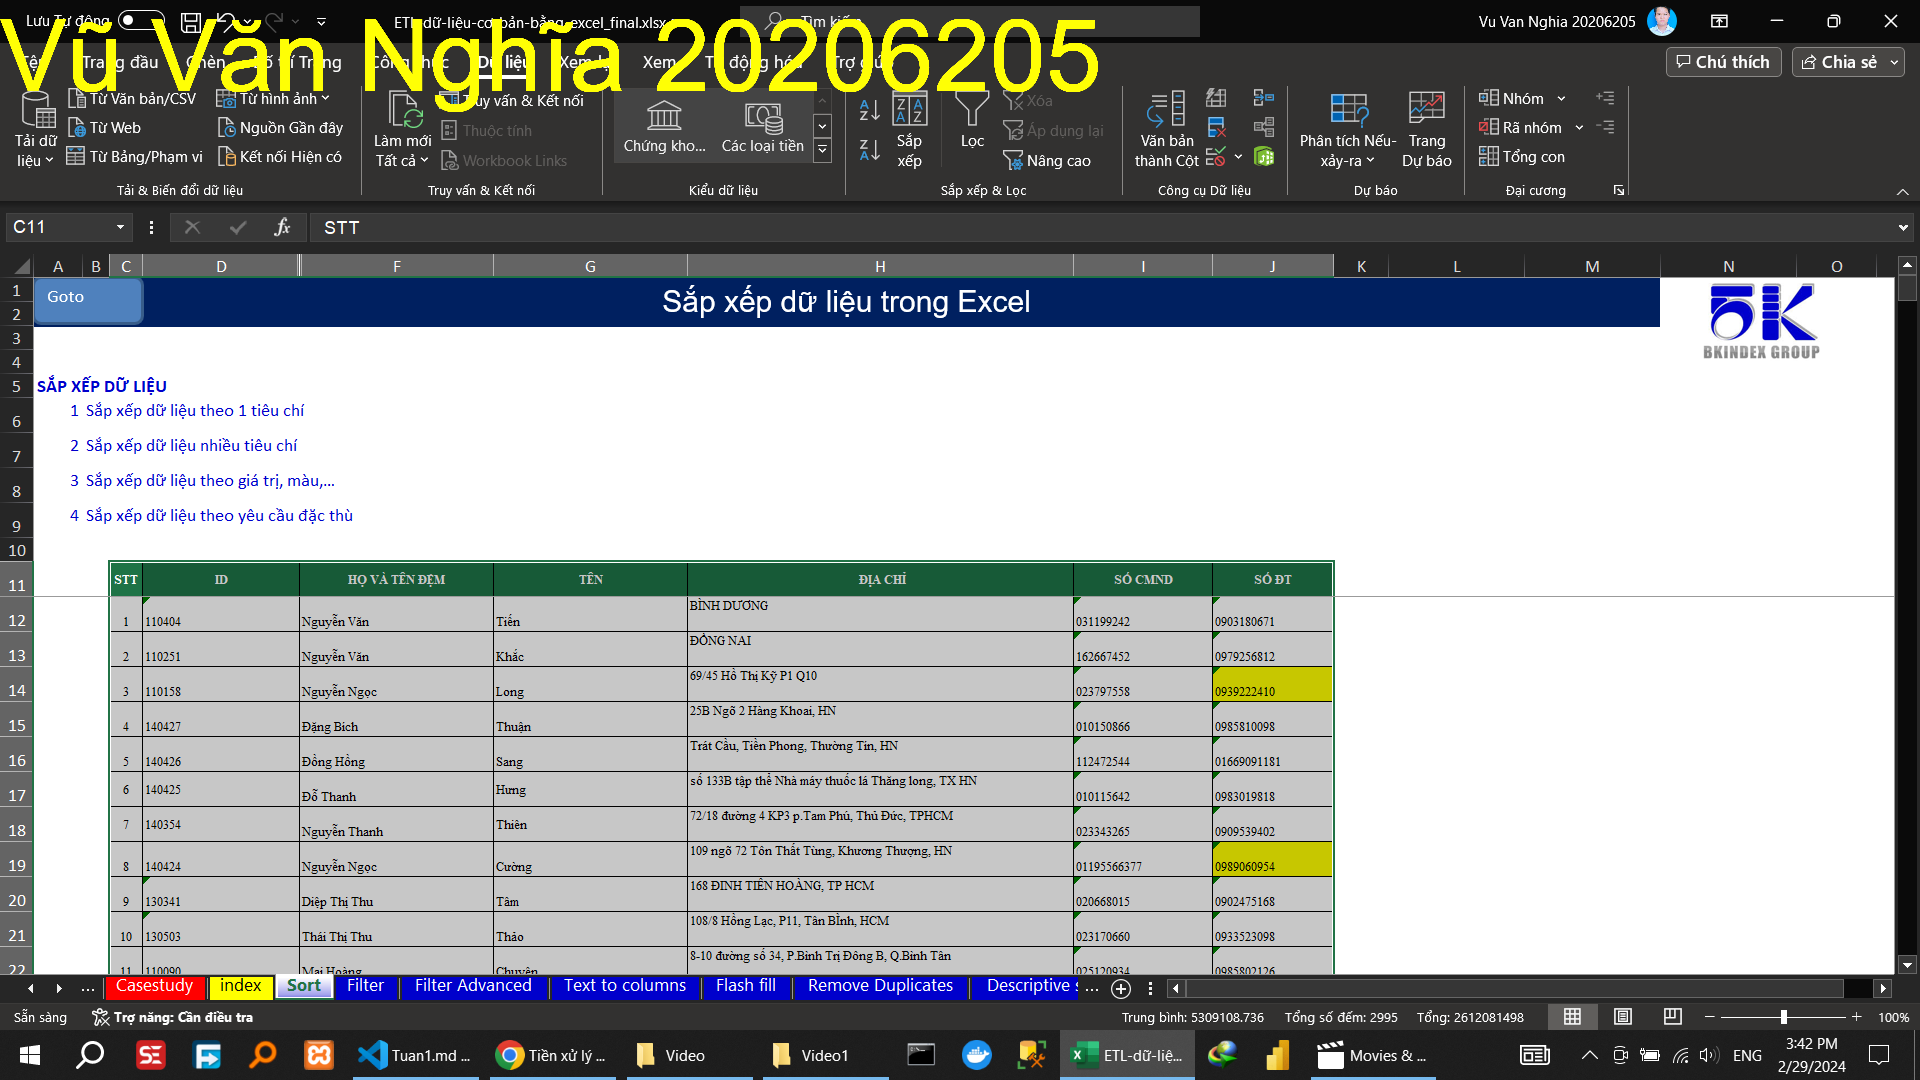
\includegraphics[scale = 0.15]{Video1/HuongDan/1.png}
    \caption{Hướng dẫn sắp xếp dữ liệu theo 1 tiêu chí là số thứ tự}
\end{figure}

\begin{figure}[h]
    \centering
    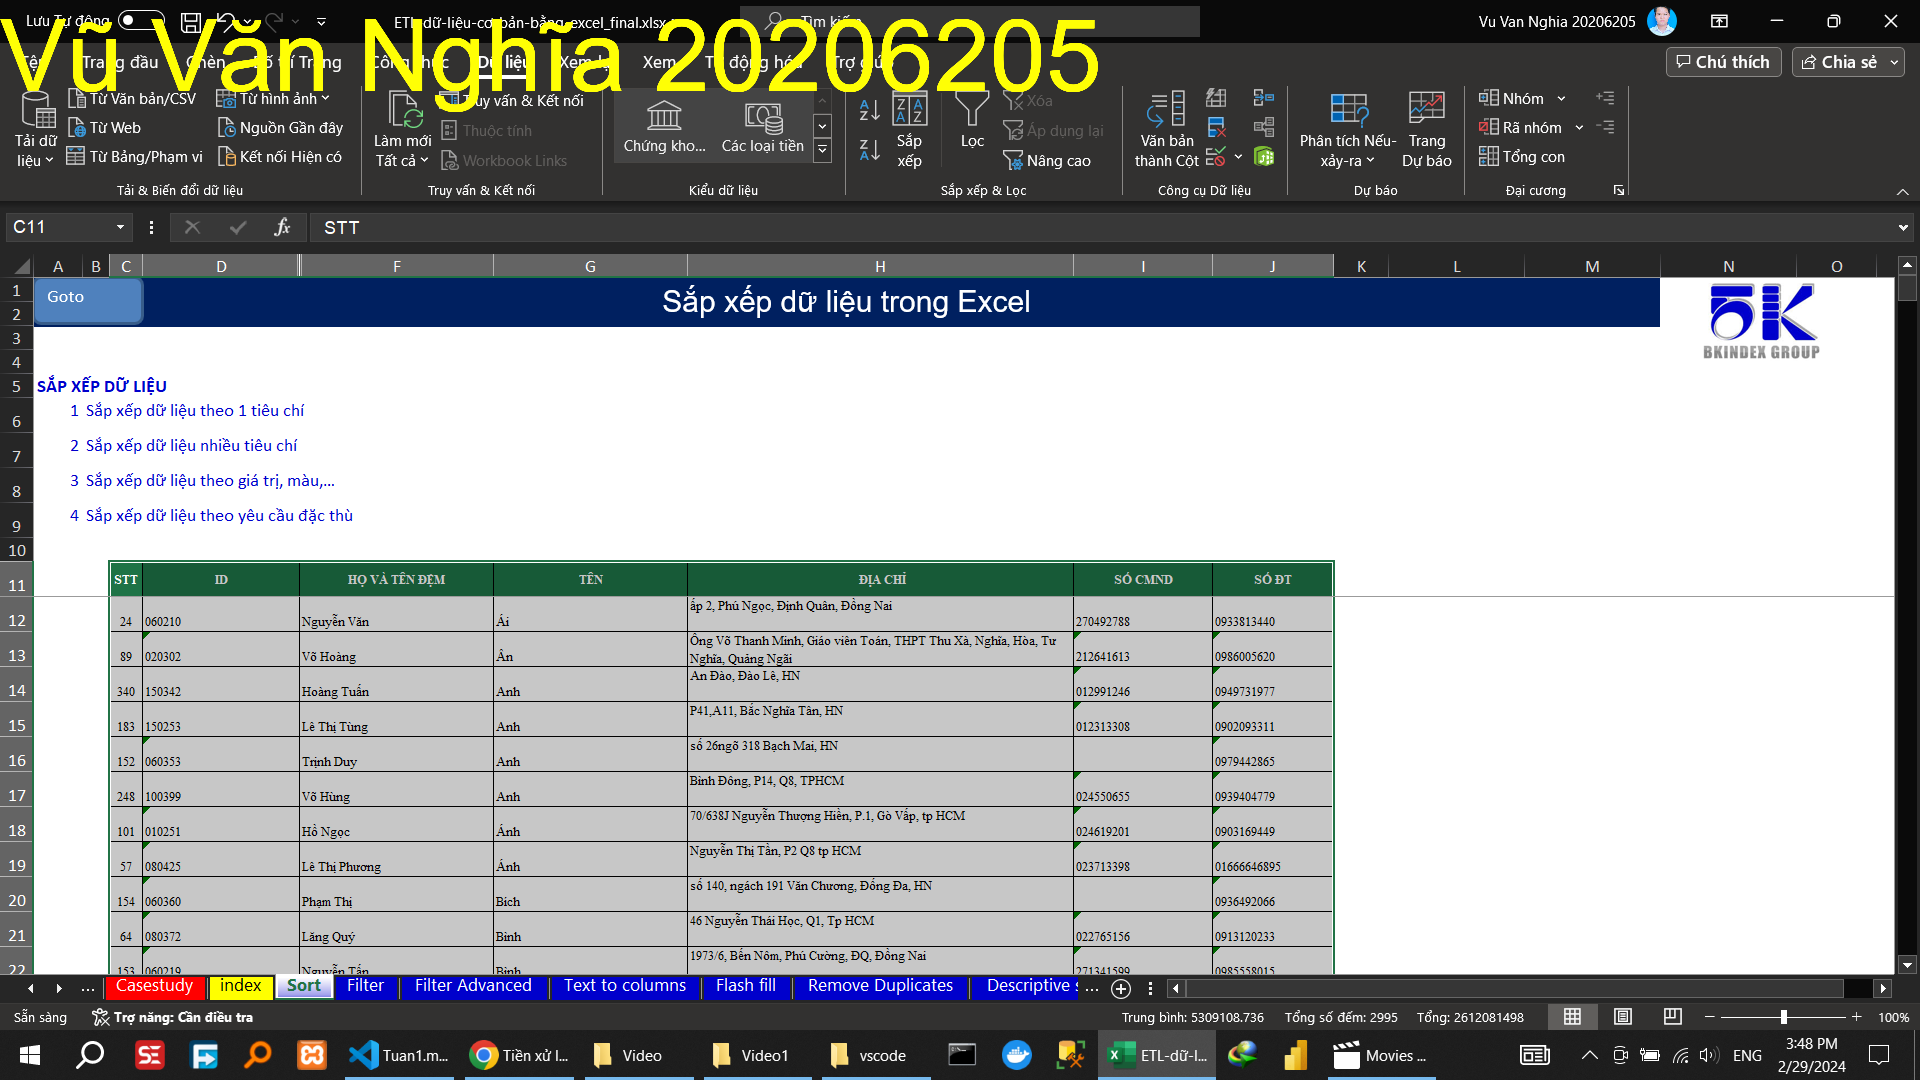
\includegraphics[scale = 0.15]{Video1/HuongDan/2.png}
    \caption{Hướng dẫn sắp xếp dữ liệu theo nhiều tiêu chí họ và tên đệm}
\end{figure}

\begin{figure}[h]
    \centering
    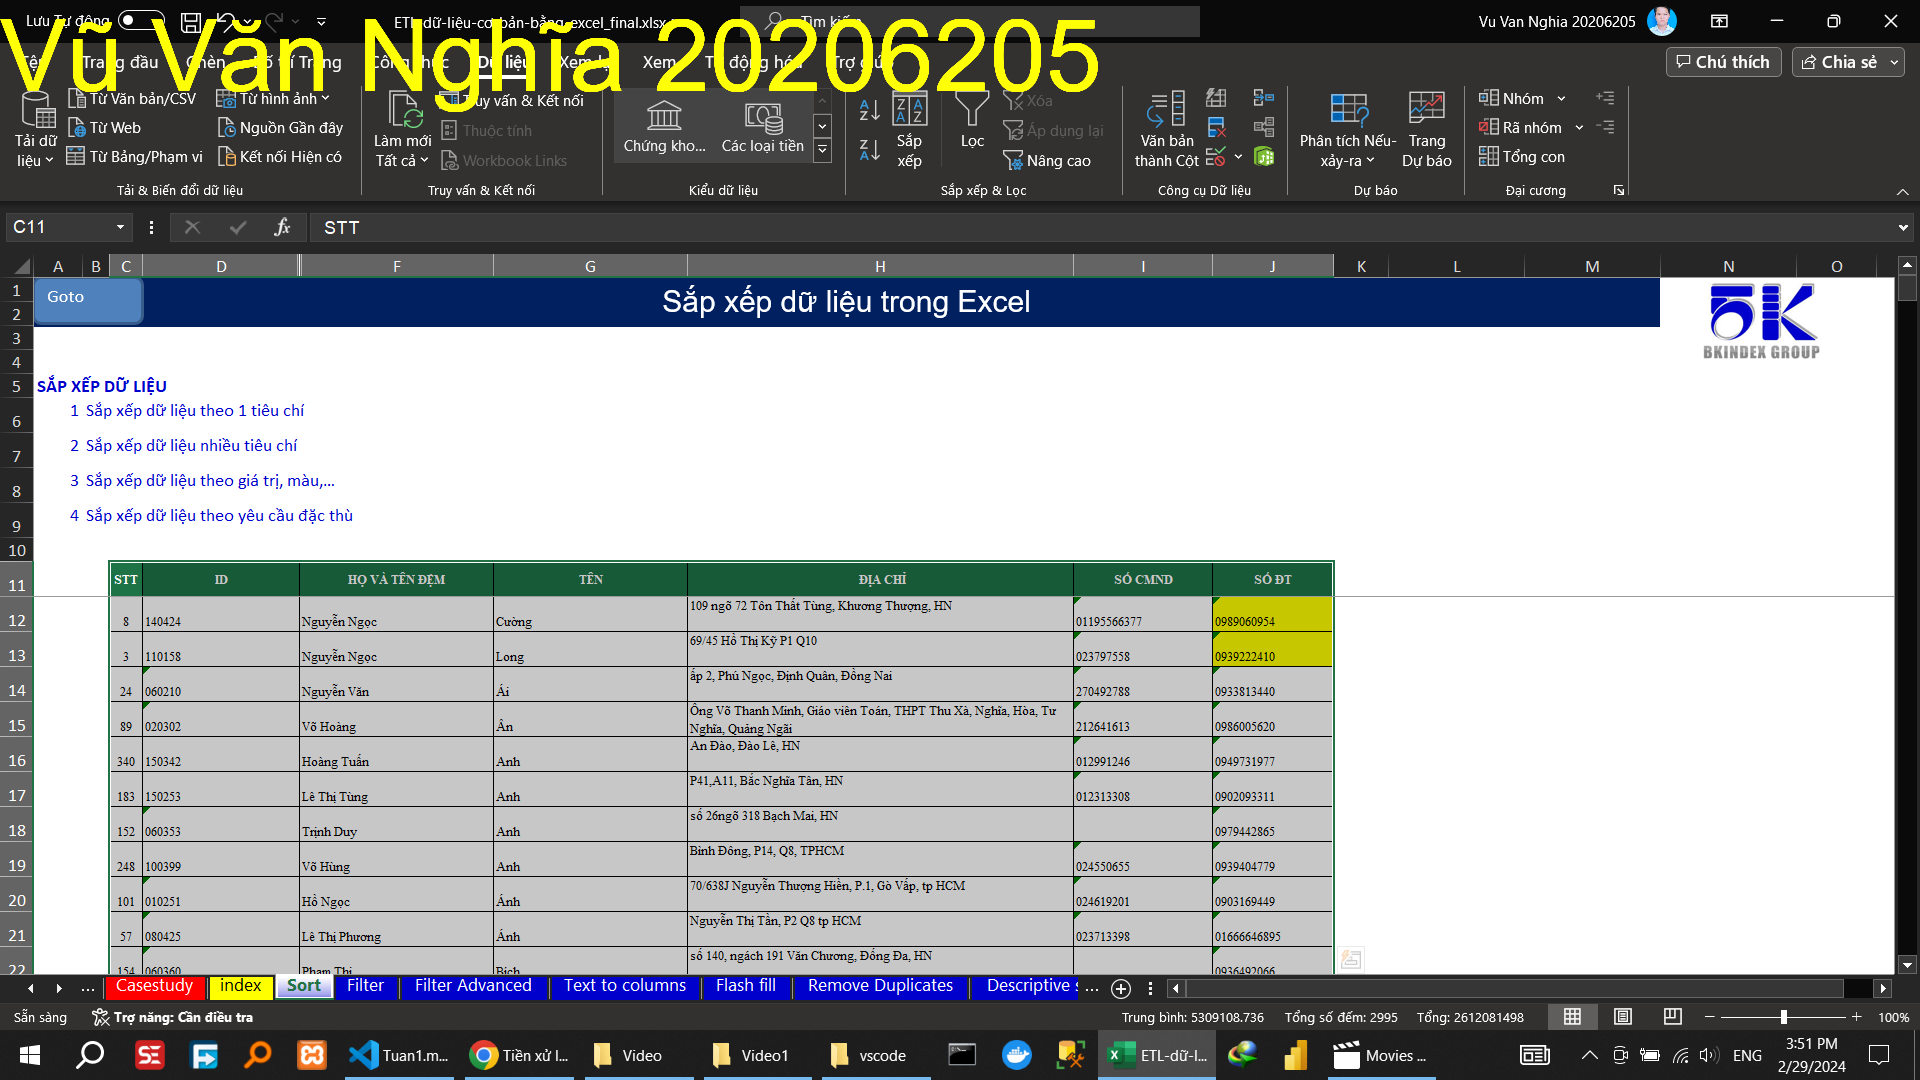
\includegraphics[scale = 0.15]{Video1/HuongDan/3.png}
    \caption{Hướng dẫn sắp xếp dữ liệu theo giá trị, màu,\dots của số điện thoại}
\end{figure}











% % \paragraph{Hướng dẫn lọc dữ liệu}
% % \subparagraph{Hướng dẫn lọc dữ liệu theo 1 tiêu chí}
% \begin{figure}[h]
%     \centering
%     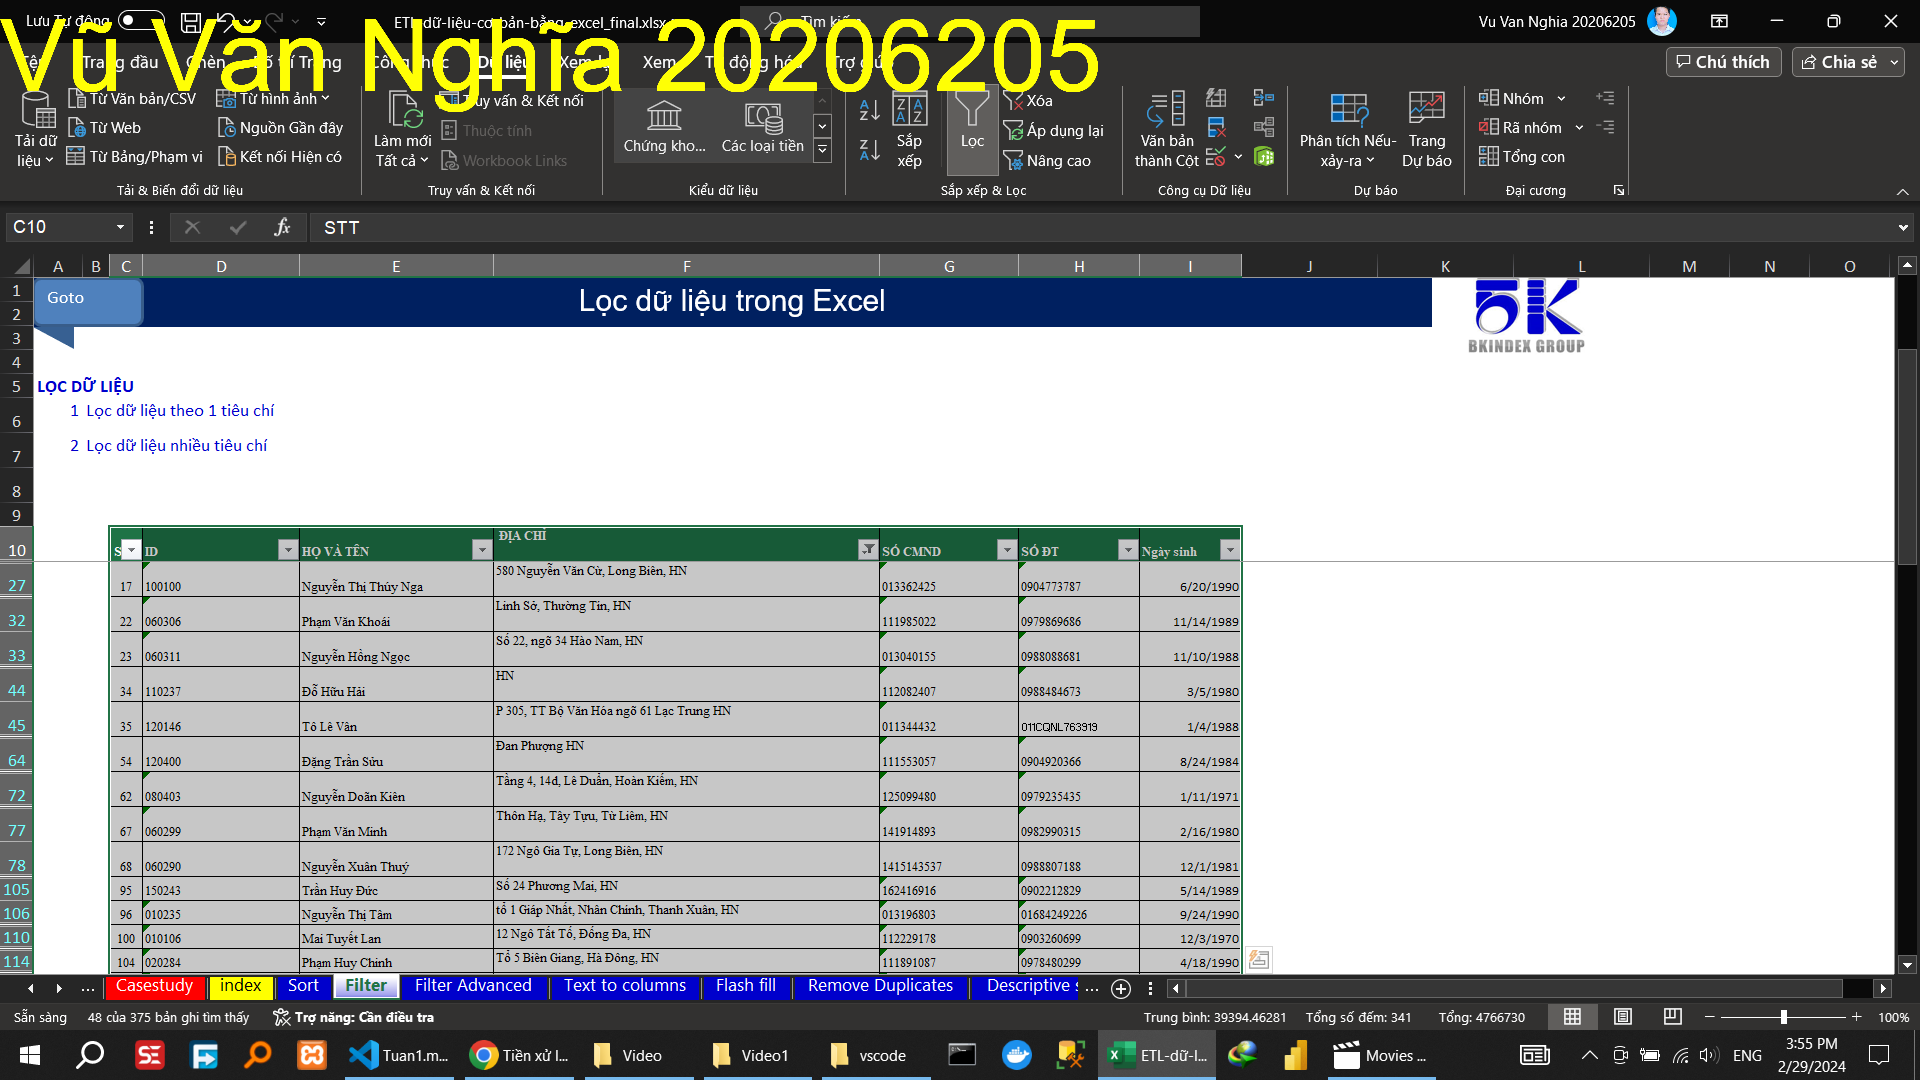
\includegraphics[scale = 0.15]{Video1/HuongDan/4.png}
%     \caption{Hướng dẫn lọc dữ liệu theo 1 tiêu chí là địa chỉ HN}
% \end{figure}
% % \subparagraph{Hướng dẫn lọc dữ liệu theo nhiều tiêu chí}
% \begin{figure}[h]
%     \centering
%     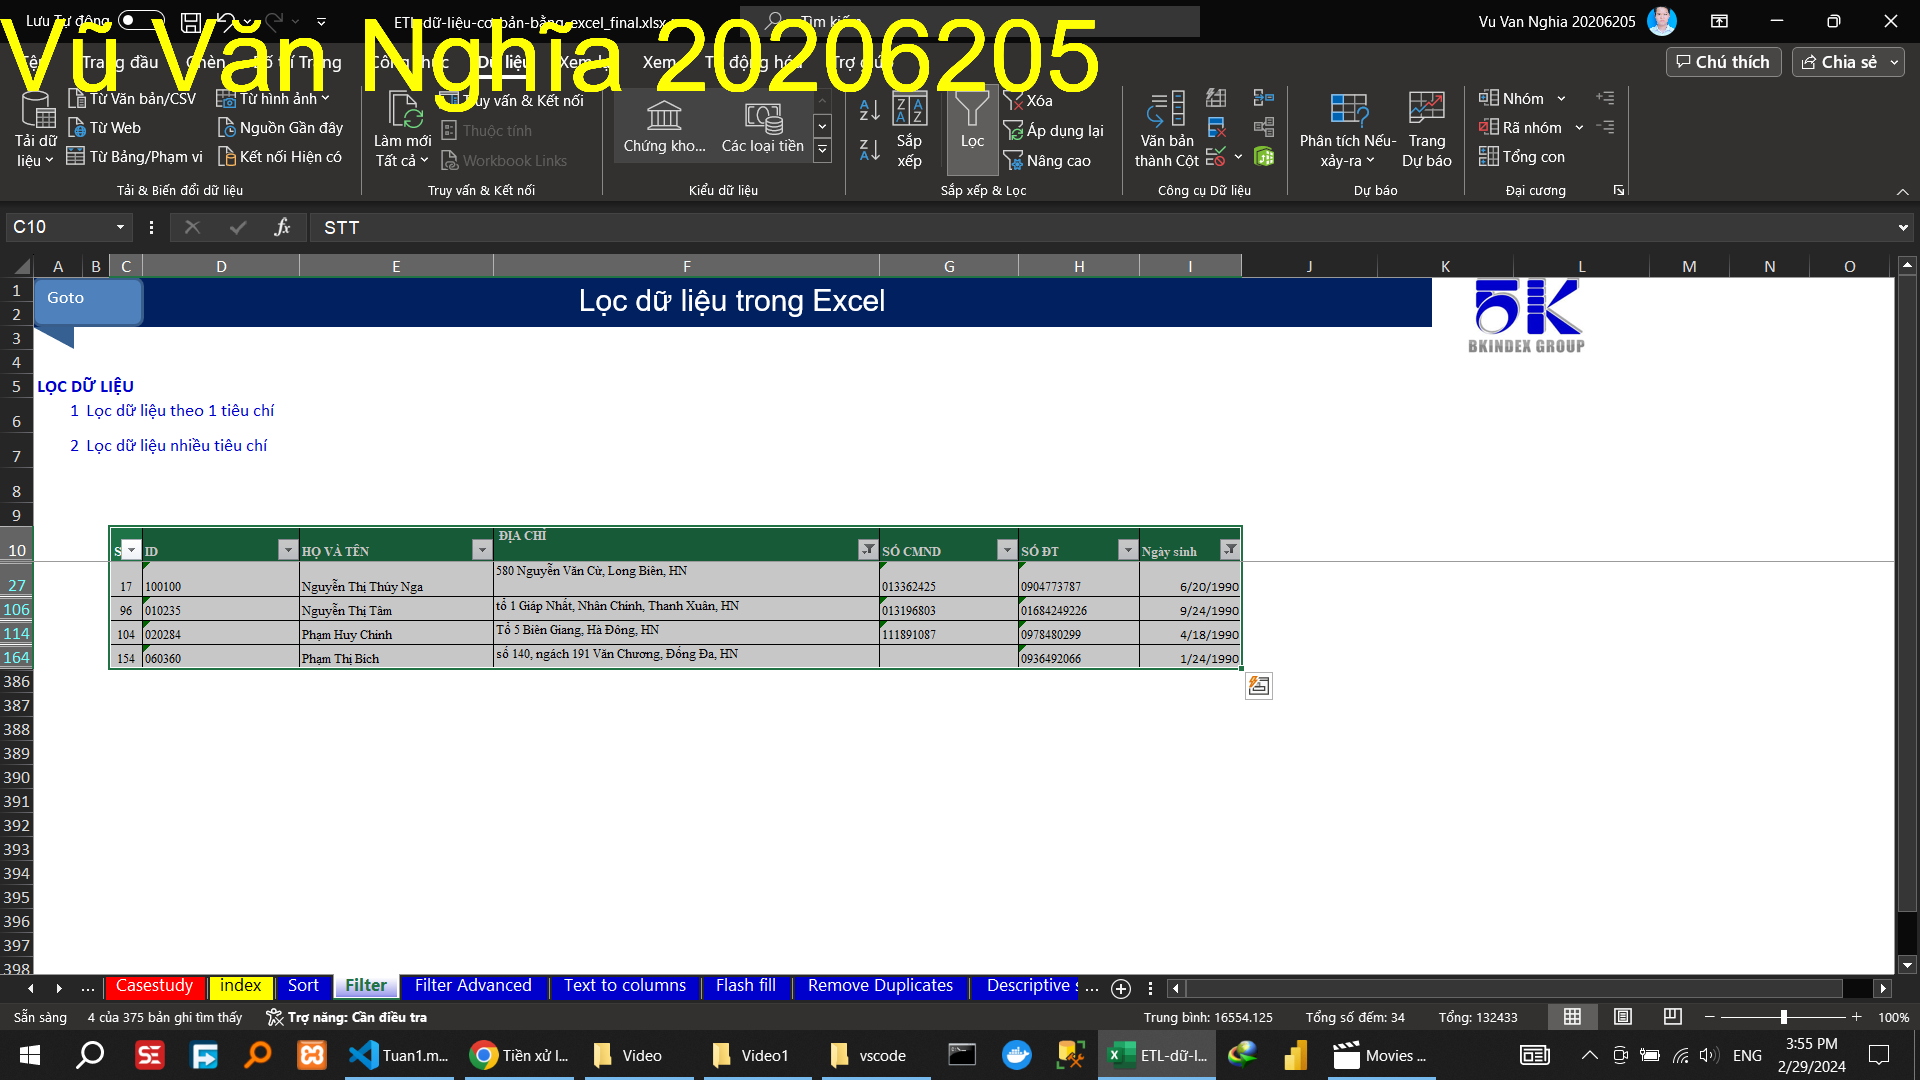
\includegraphics[scale = 0.15]{Video1/HuongDan/5.png}
%     \caption{Hướng dẫn lọc dữ liệu theo nhiều tiêu chí địa chỉ và sinh năm 1990}
% \end{figure}

% % \paragraph{Hướng dẫn lọc dữ liệu nâng cao}
% % \subparagraph{Hướng dẫn lọc dữ liệu nâng cao theo 1 tiêu chí}
% \begin{figure}[h]
%     \centering
%     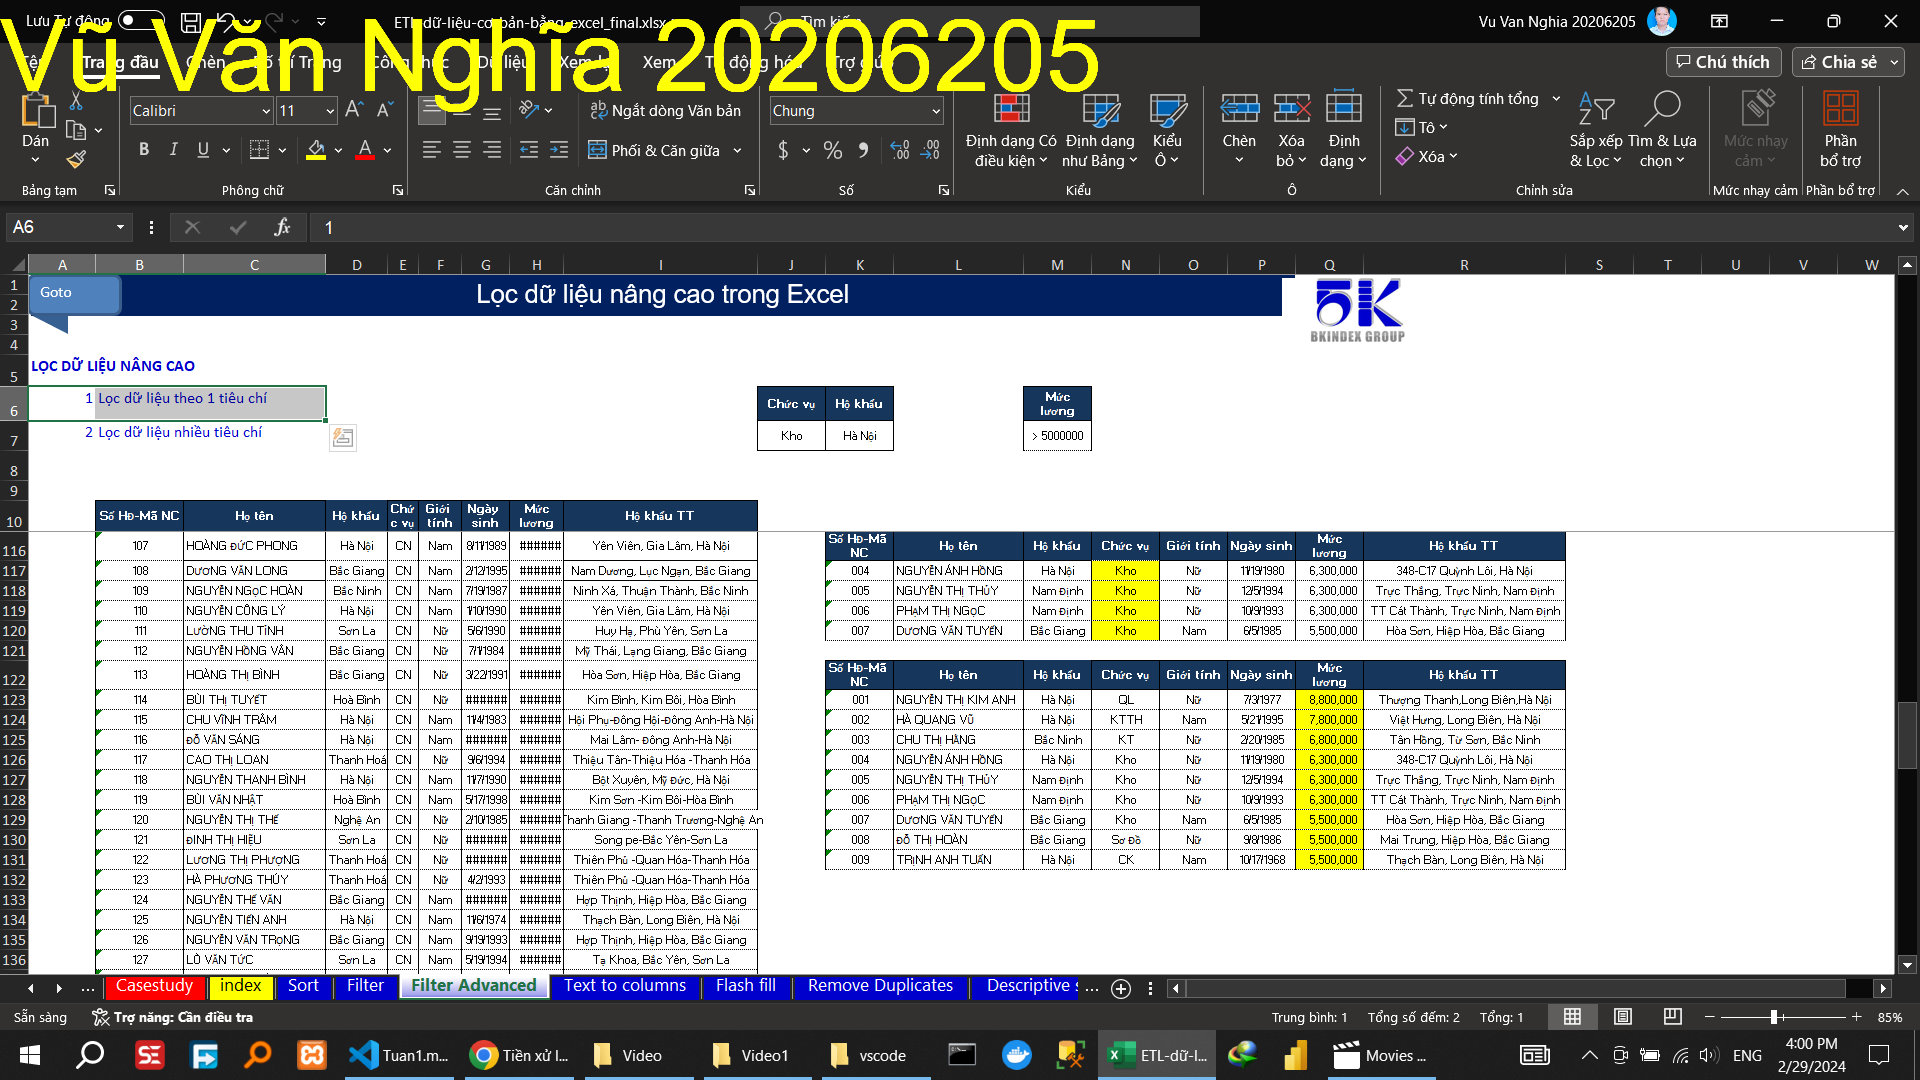
\includegraphics[scale = 0.15]{Video1/HuongDan/6.png}
%     \caption{Hướng dẫn lọc dữ liệu nâng cao theo 1 tiêu chí là chức vụ hoặc mức lương}
% \end{figure}
% % \subparagraph{Hướng dẫn lọc dữ liệu nâng cao theo nhiều tiêu chí}
% \begin{figure}[h]
%     \centering
%     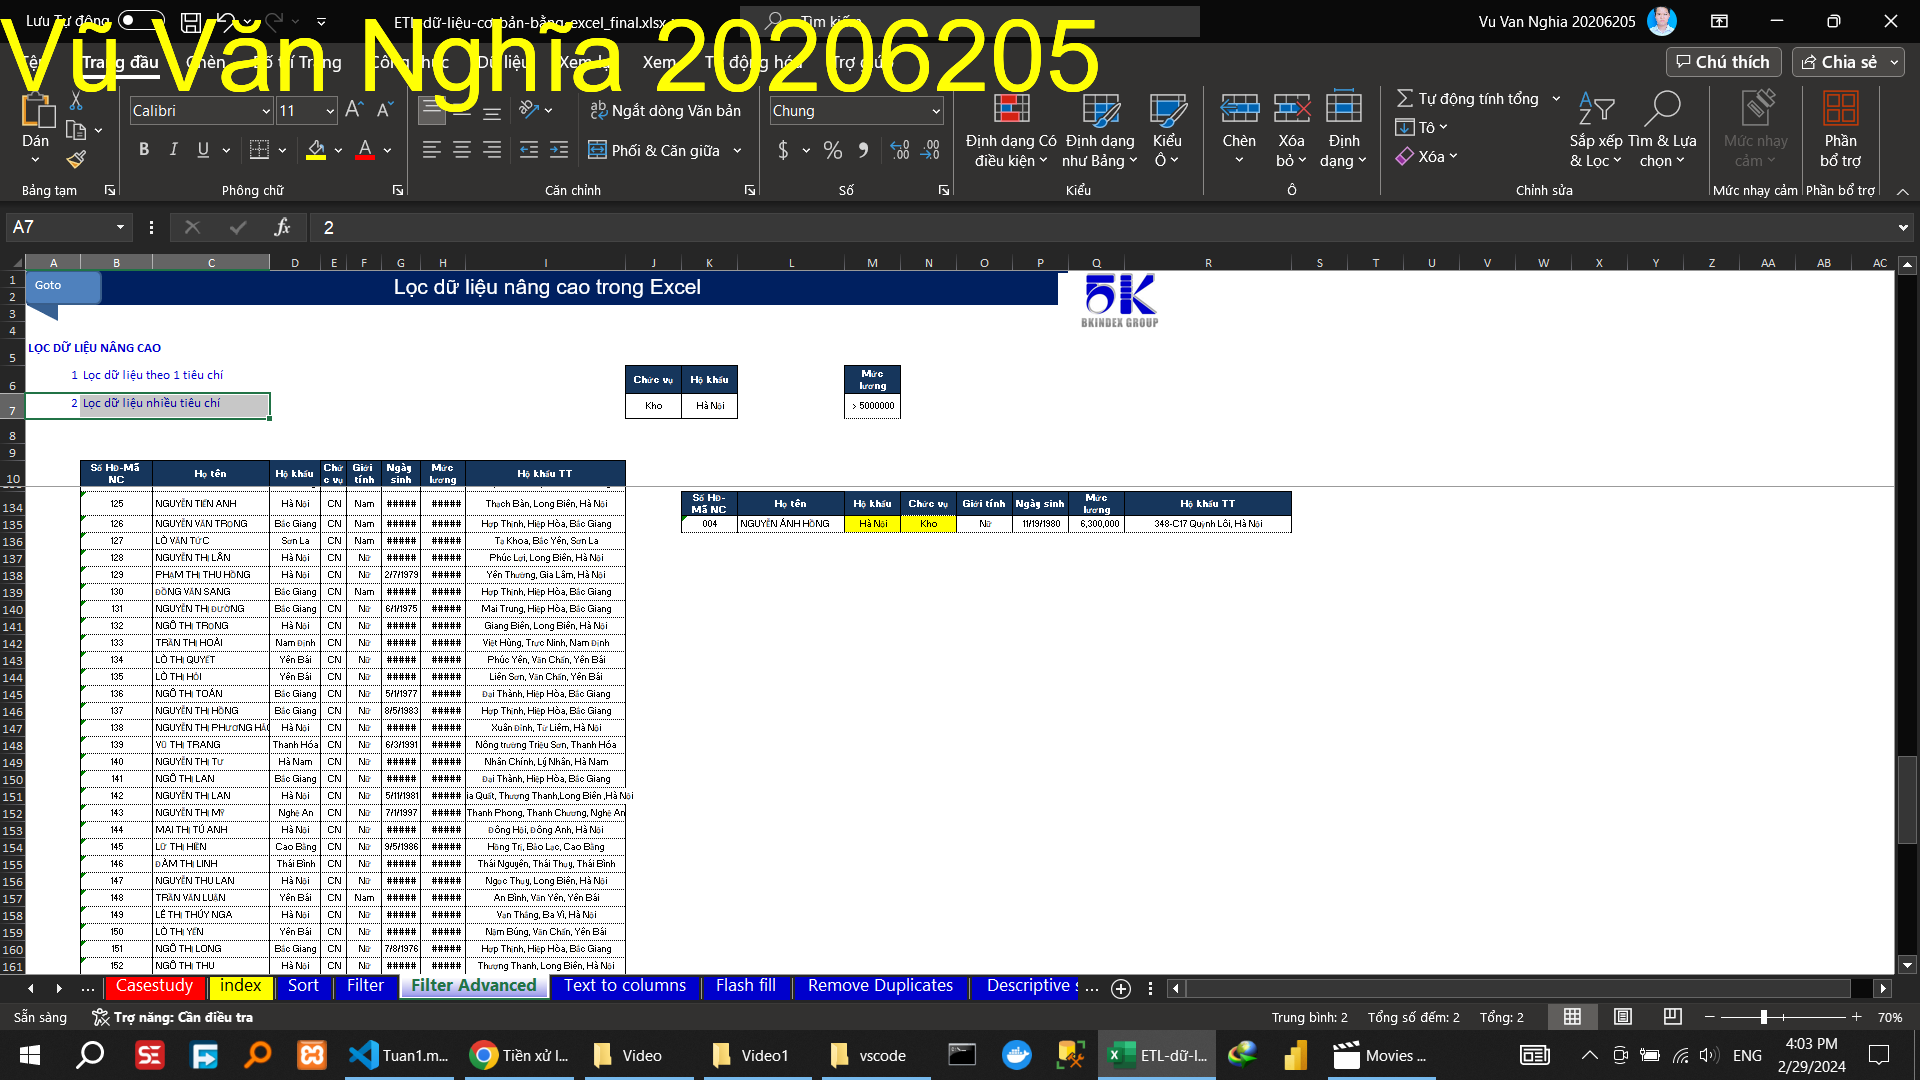
\includegraphics[scale = 0.15]{Video1/HuongDan/7.png}
%     \caption{Hướng dẫn lọc dữ liệu nâng cao theo nhiều tiêu chí chức vụ và hộ khẩu}
% \end{figure}

% % \paragraph{Hướng dẫn tách cột văn bản thành nhiều cột}
% % \subparagraph{Hướng dẫn tách ngày tháng}
% \begin{figure}[h]
%     \centering
%     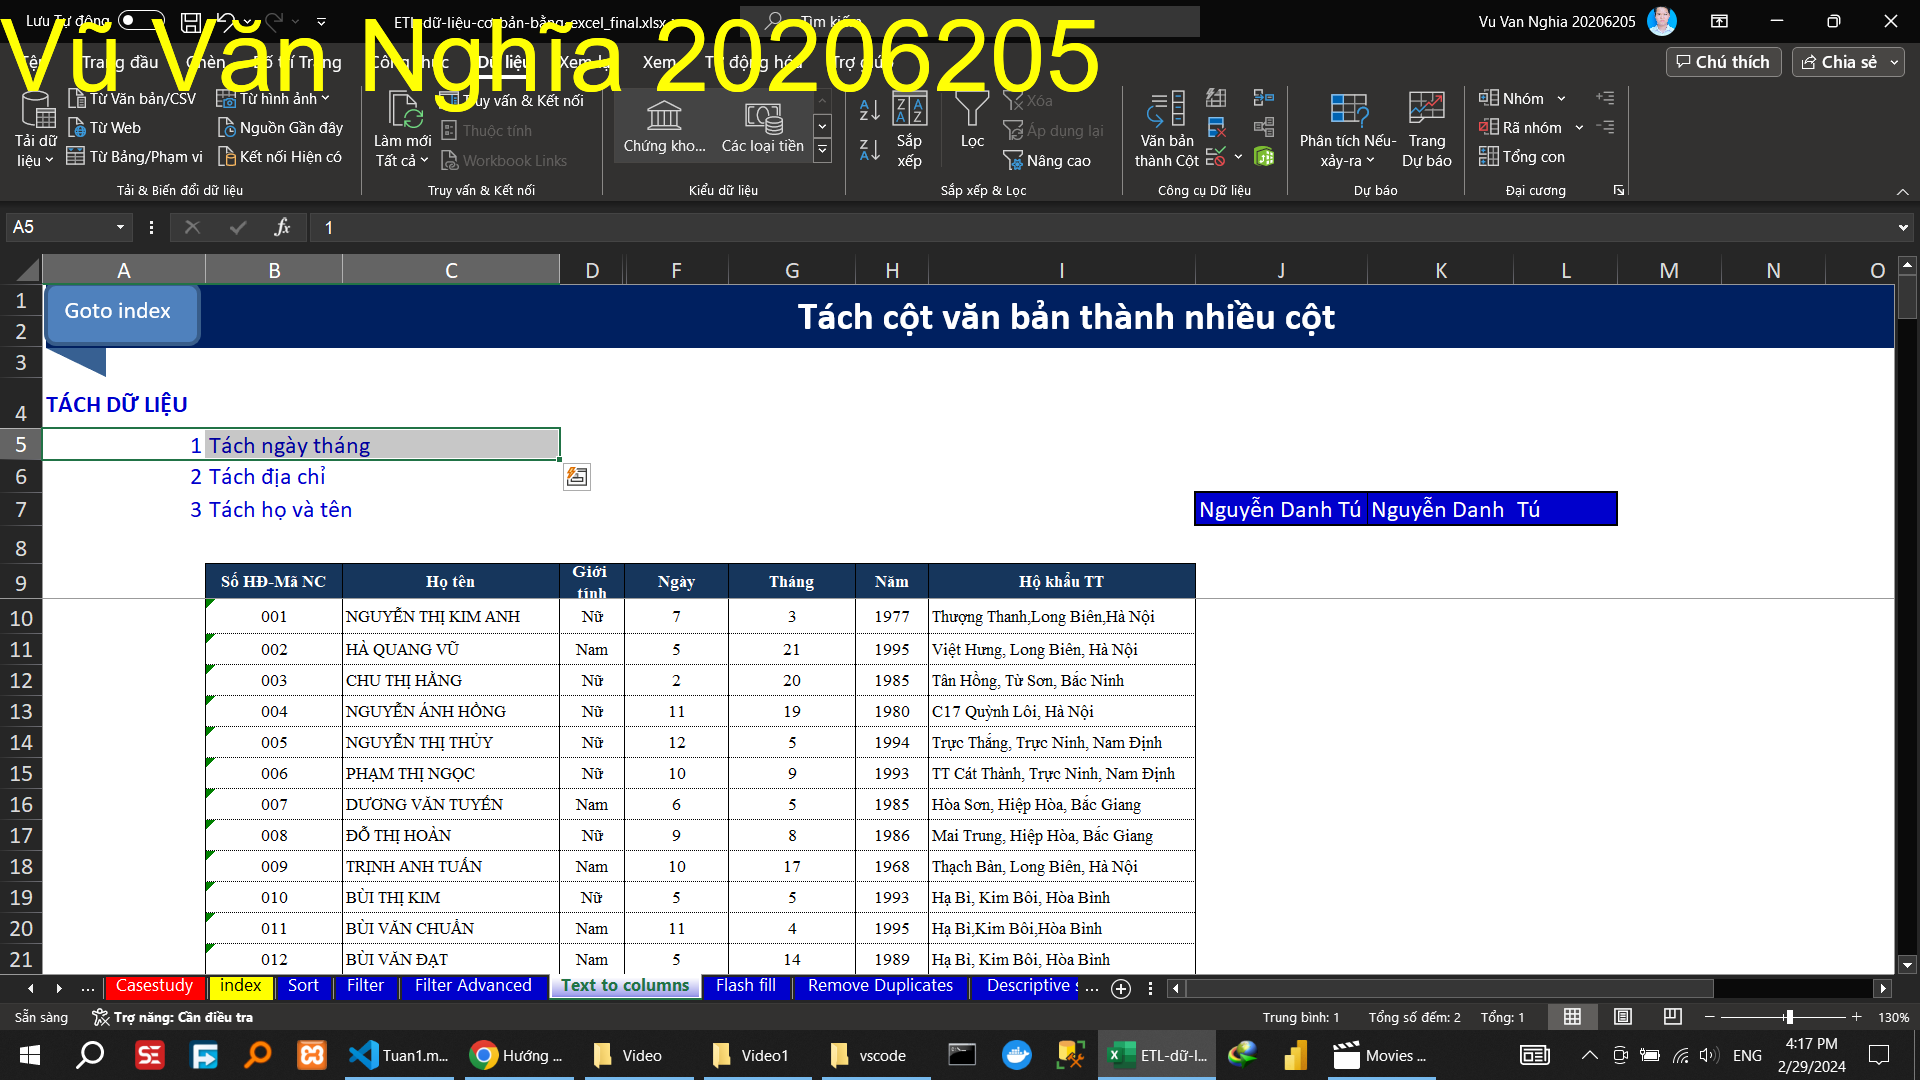
\includegraphics[scale = 0.15]{Video1/HuongDan/8.png}
%     \caption{Hướng dẫn tách ngày tháng}
% \end{figure}
% % \subparagraph{Hướng dẫn tách địa chỉ}
% \begin{figure}[h]
%     \centering
%     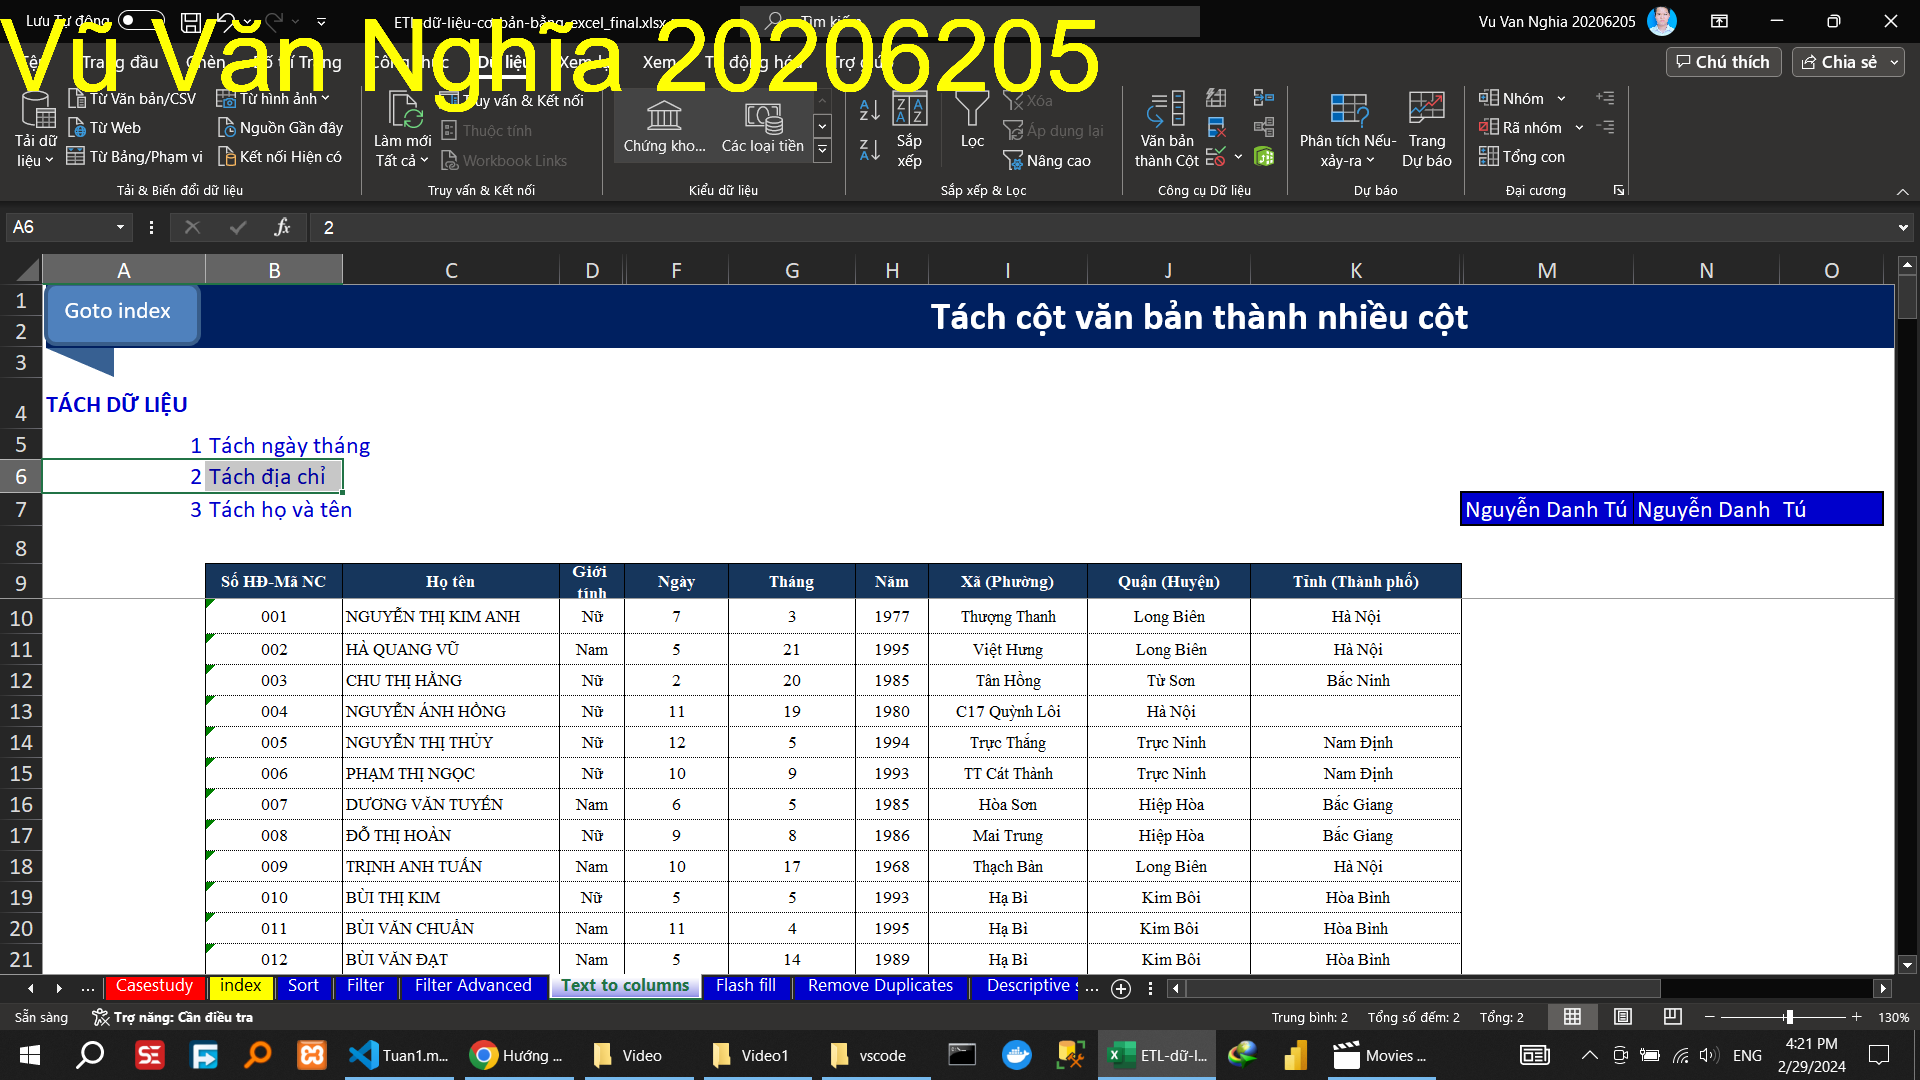
\includegraphics[scale = 0.15]{Video1/HuongDan/9.png}
%     \caption{Hướng dẫn tách địa chỉ}
% \end{figure}
% % \subparagraph{Hướng dẫn tách họ và tên}
% \begin{figure}[h]
%     \centering
%     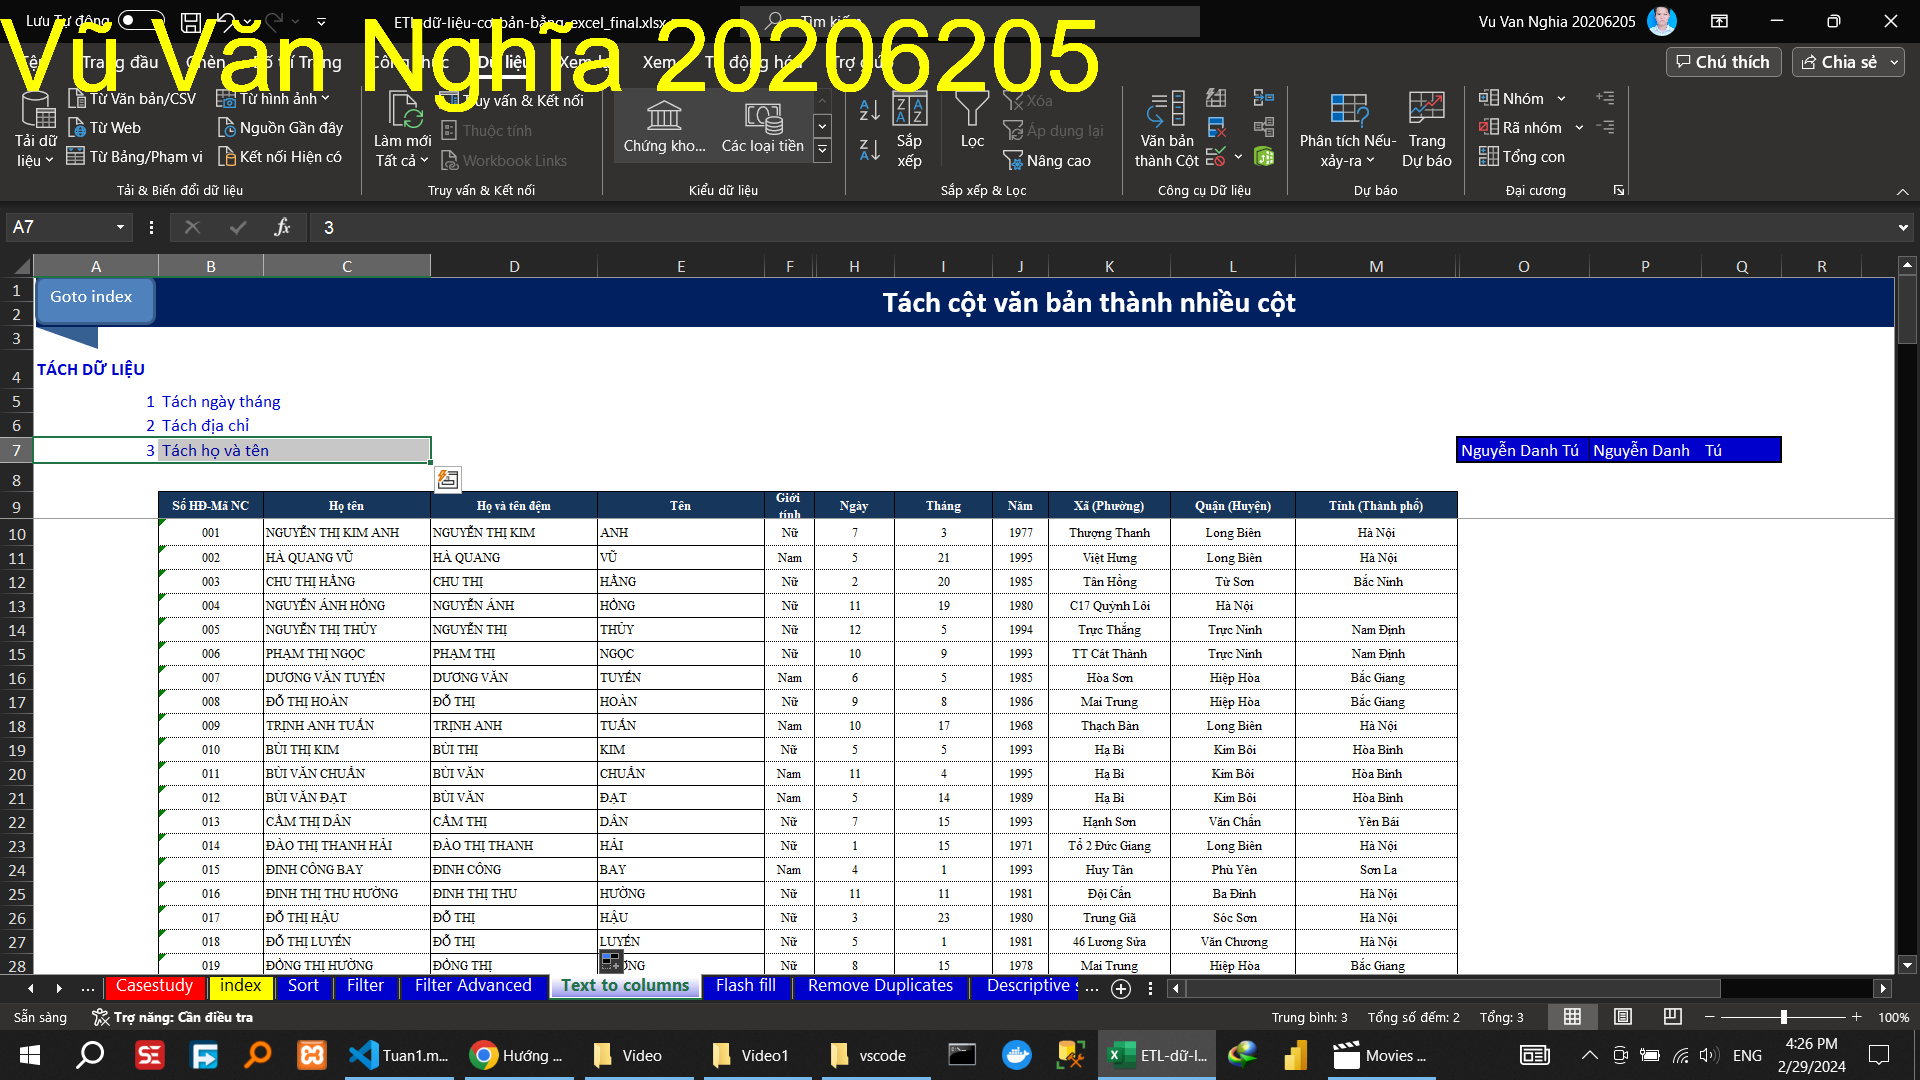
\includegraphics[scale = 0.15]{Video1/HuongDan/10.png}
%     \caption{Hướng dẫn tách họ và tên}
% \end{figure}

% % \paragraph{Hướng dẫn điền dữ liệu tự động}
% % \subparagraph{Hướng dẫn điền dữ liệu tự động}
% \begin{figure}[h]
%     \centering
%     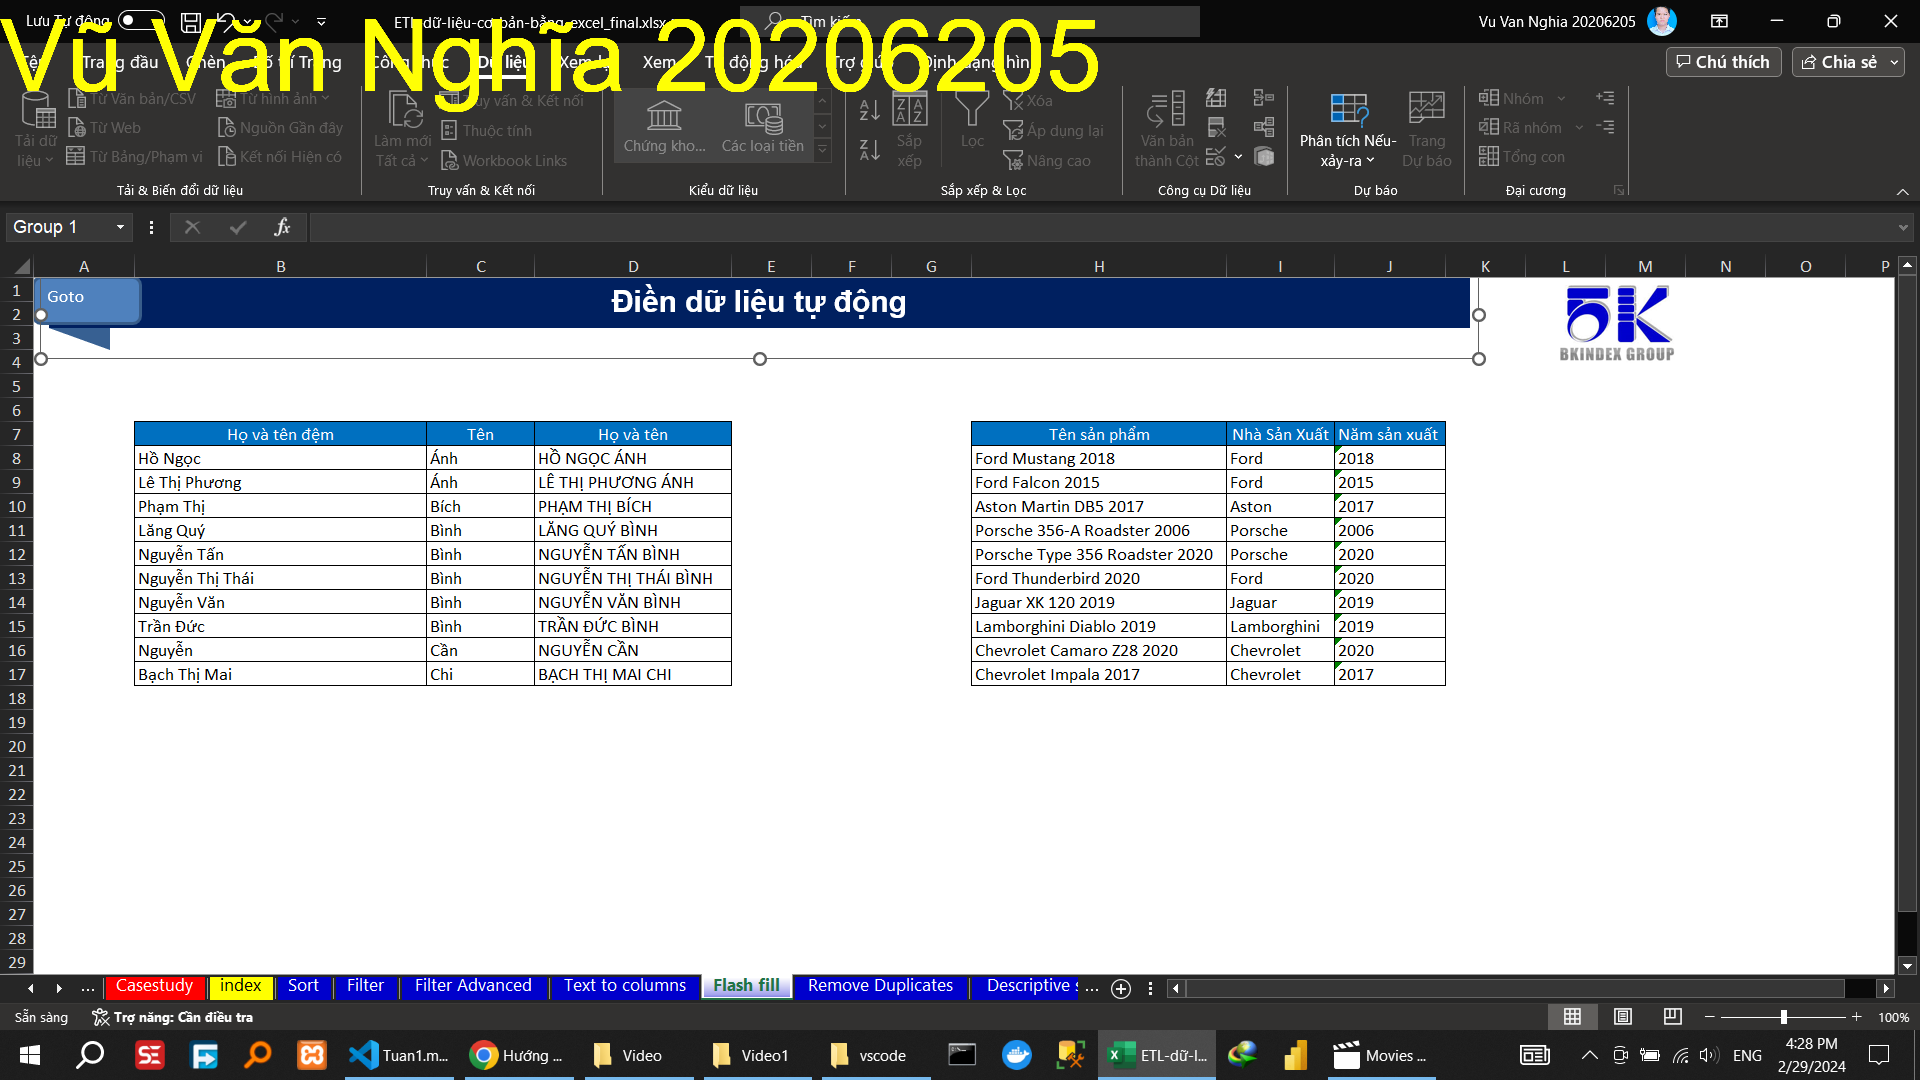
\includegraphics[scale = 0.15]{Video1/HuongDan/11.png}
%     \caption{Hướng dẫn điền dữ liệu tự động}
% \end{figure}

% % \paragraph{Hướng dẫn xóa dữ liệu bị trùng}
% % \subparagraph{Hướng dẫn xóa dữ liệu bị trùng}
% \begin{figure}[h]
%     \centering
%     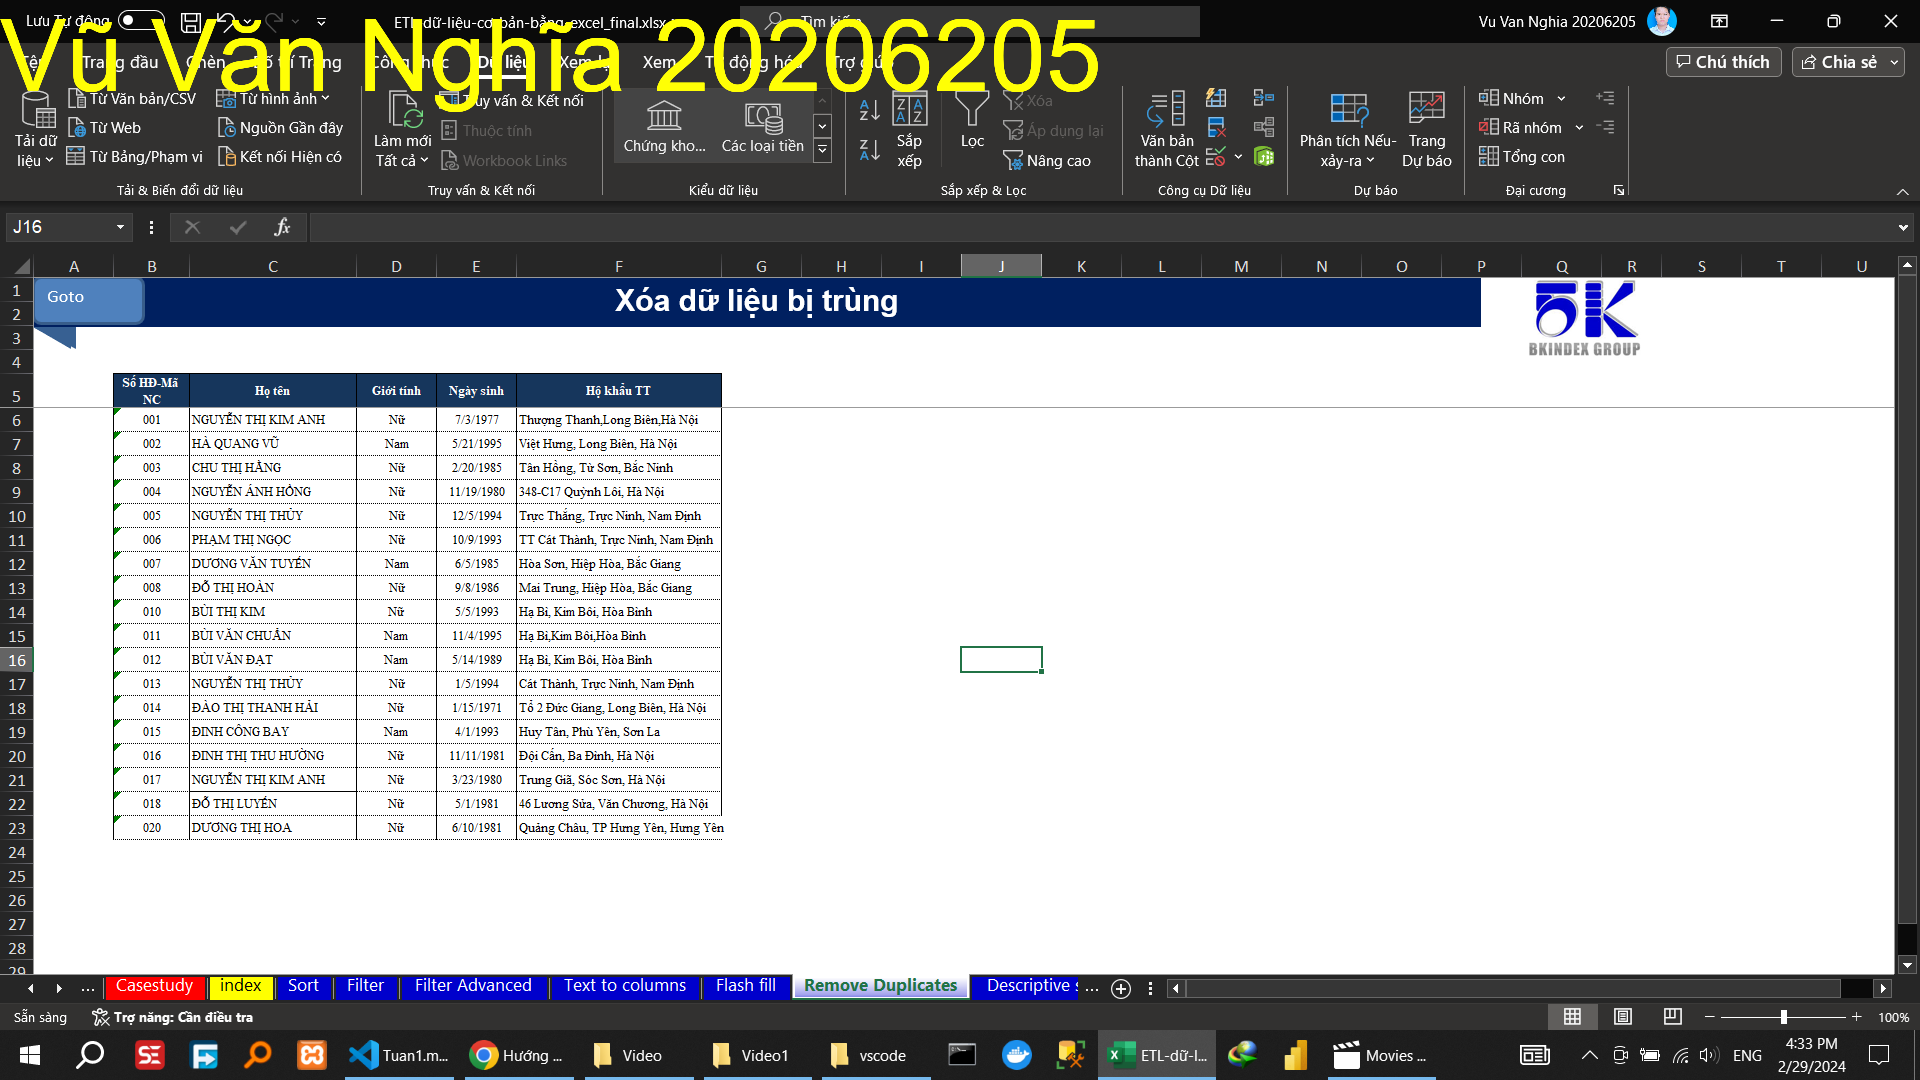
\includegraphics[scale = 0.15]{Video1/HuongDan/12.png}
%     \caption{Hướng dẫn xóa dữ liệu bị trùng}
% \end{figure}

% % \paragraph{Hướng dẫn thống kê mô tả}
% % \subparagraph{Hướng dẫn thống kê mô tả}
% \begin{figure}[h]
%     \centering
%     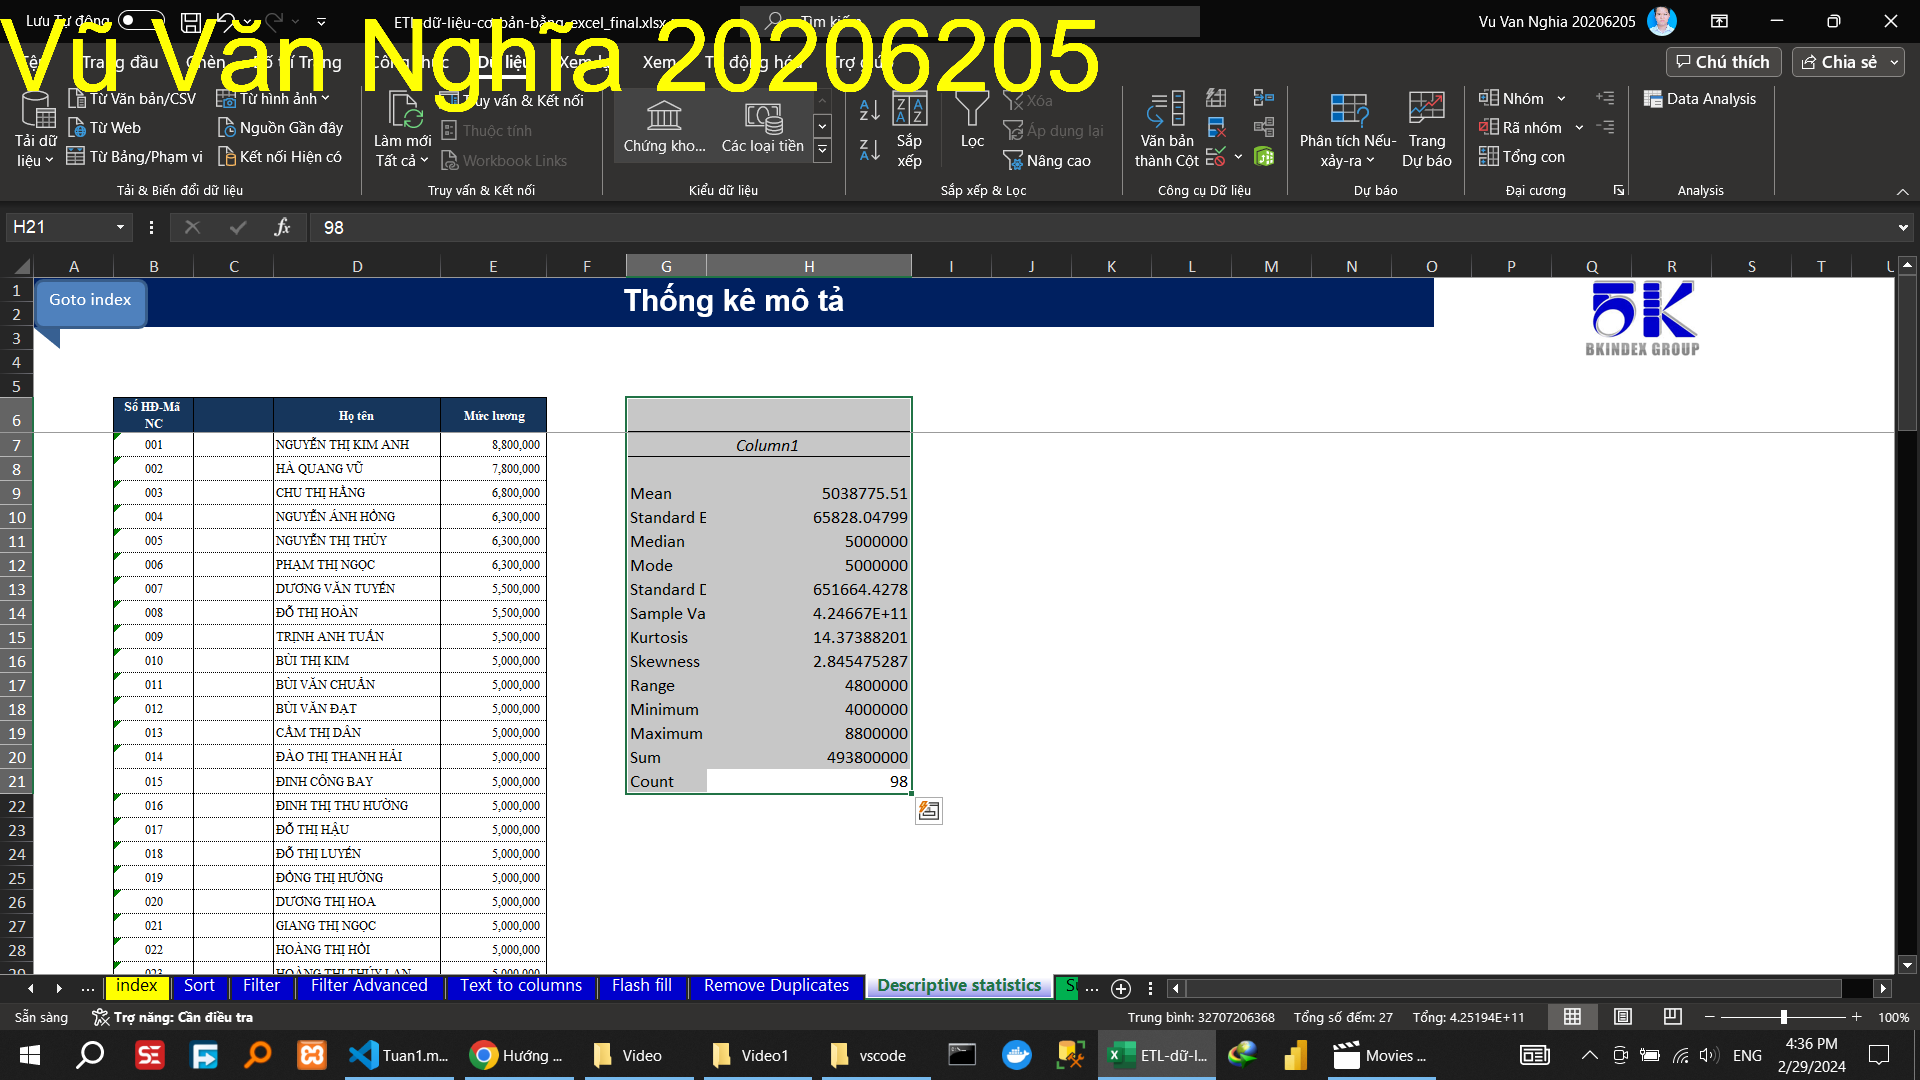
\includegraphics[scale = 0.15]{Video1/HuongDan/13.png}
%     \caption{Hướng dẫn thống kê mô tả}
% \end{figure}

% % \subsubsection{Thực hành}
% % \paragraph{Thực hành bỏ vùng trộn (merge)}
% % \subparagraph{Thực hành bỏ vùng trộn (merge)}
% \begin{figure}[h]
%     \centering
%     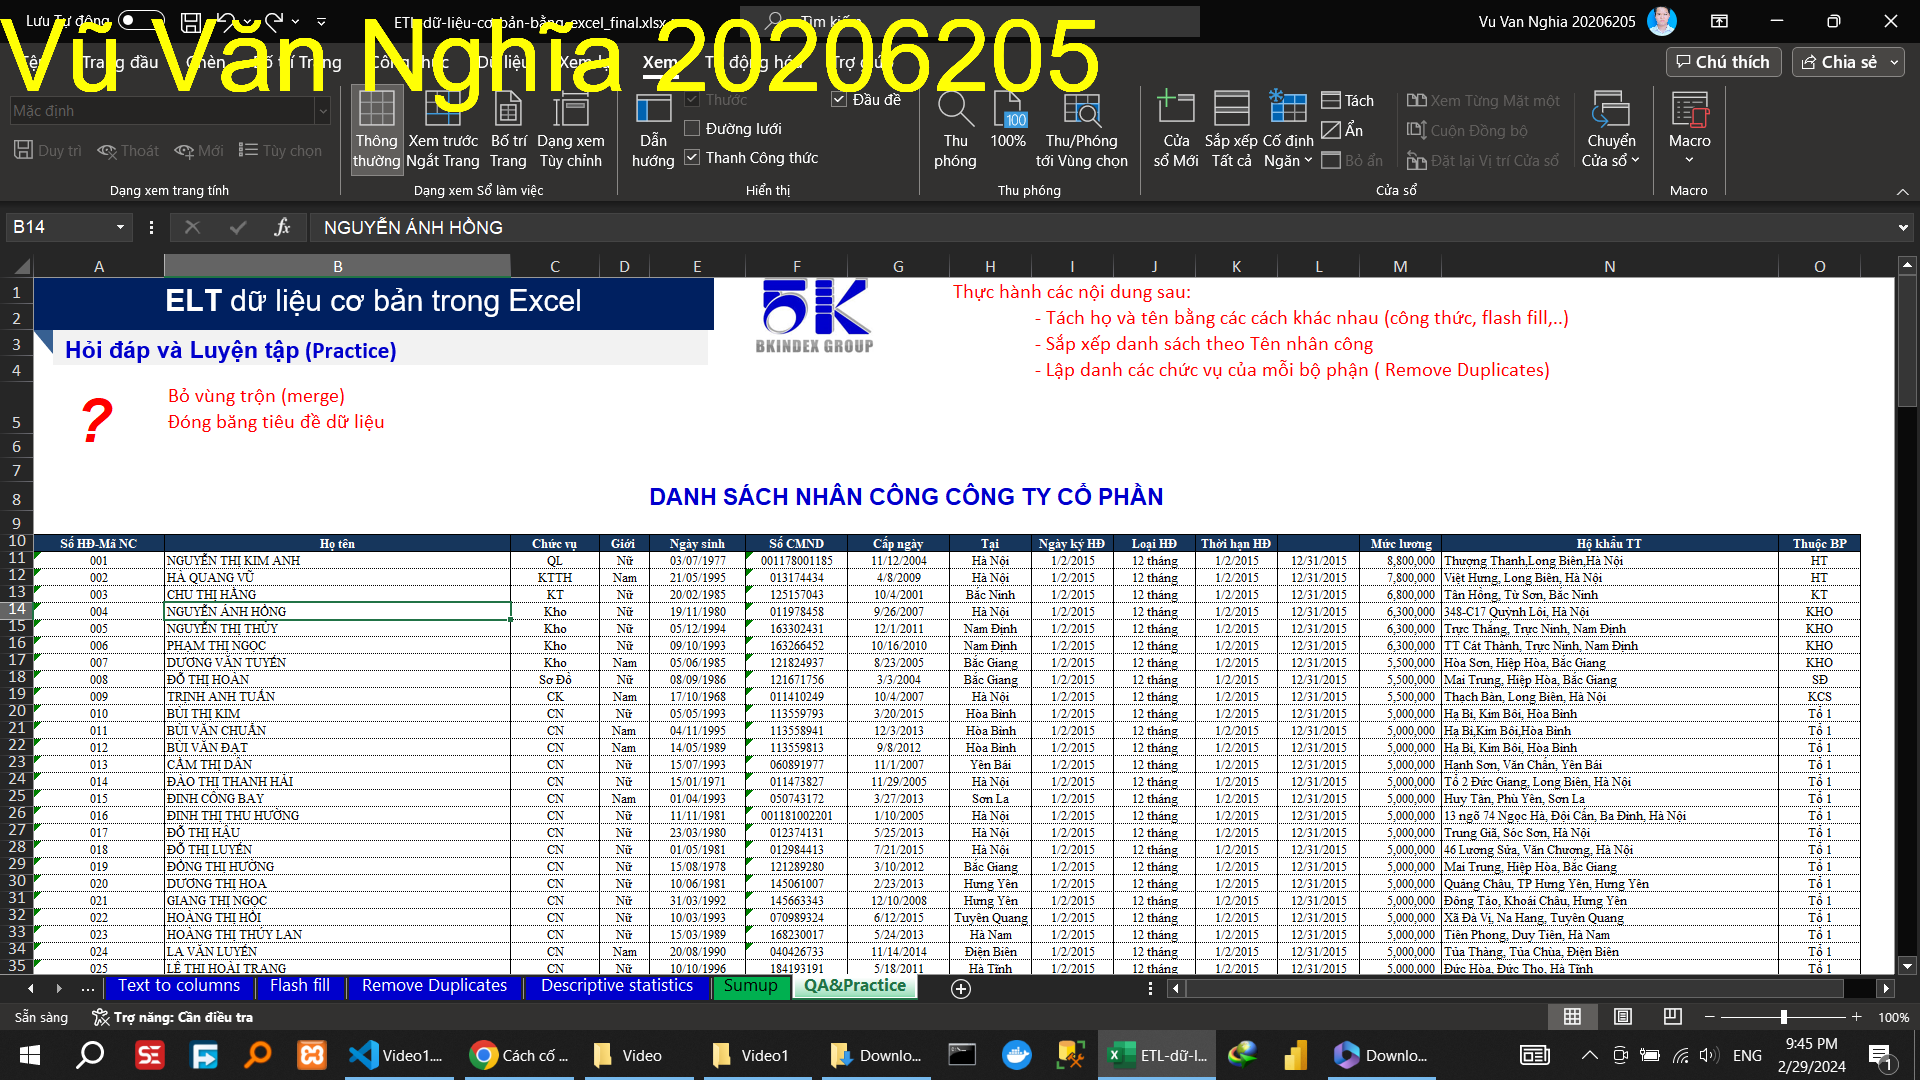
\includegraphics[scale = 0.15]{Video1/ThucHanh/1.png}
%     \caption{Thực hành bỏ vùng trộn (merge)}
% \end{figure}

% % \paragraph{Thực hành đóng băng tiêu đề dữ liệu}
% % \subparagraph{Thực hành đóng băng tiêu đề dữ liệu}
% \begin{figure}[h]
%     \centering
%     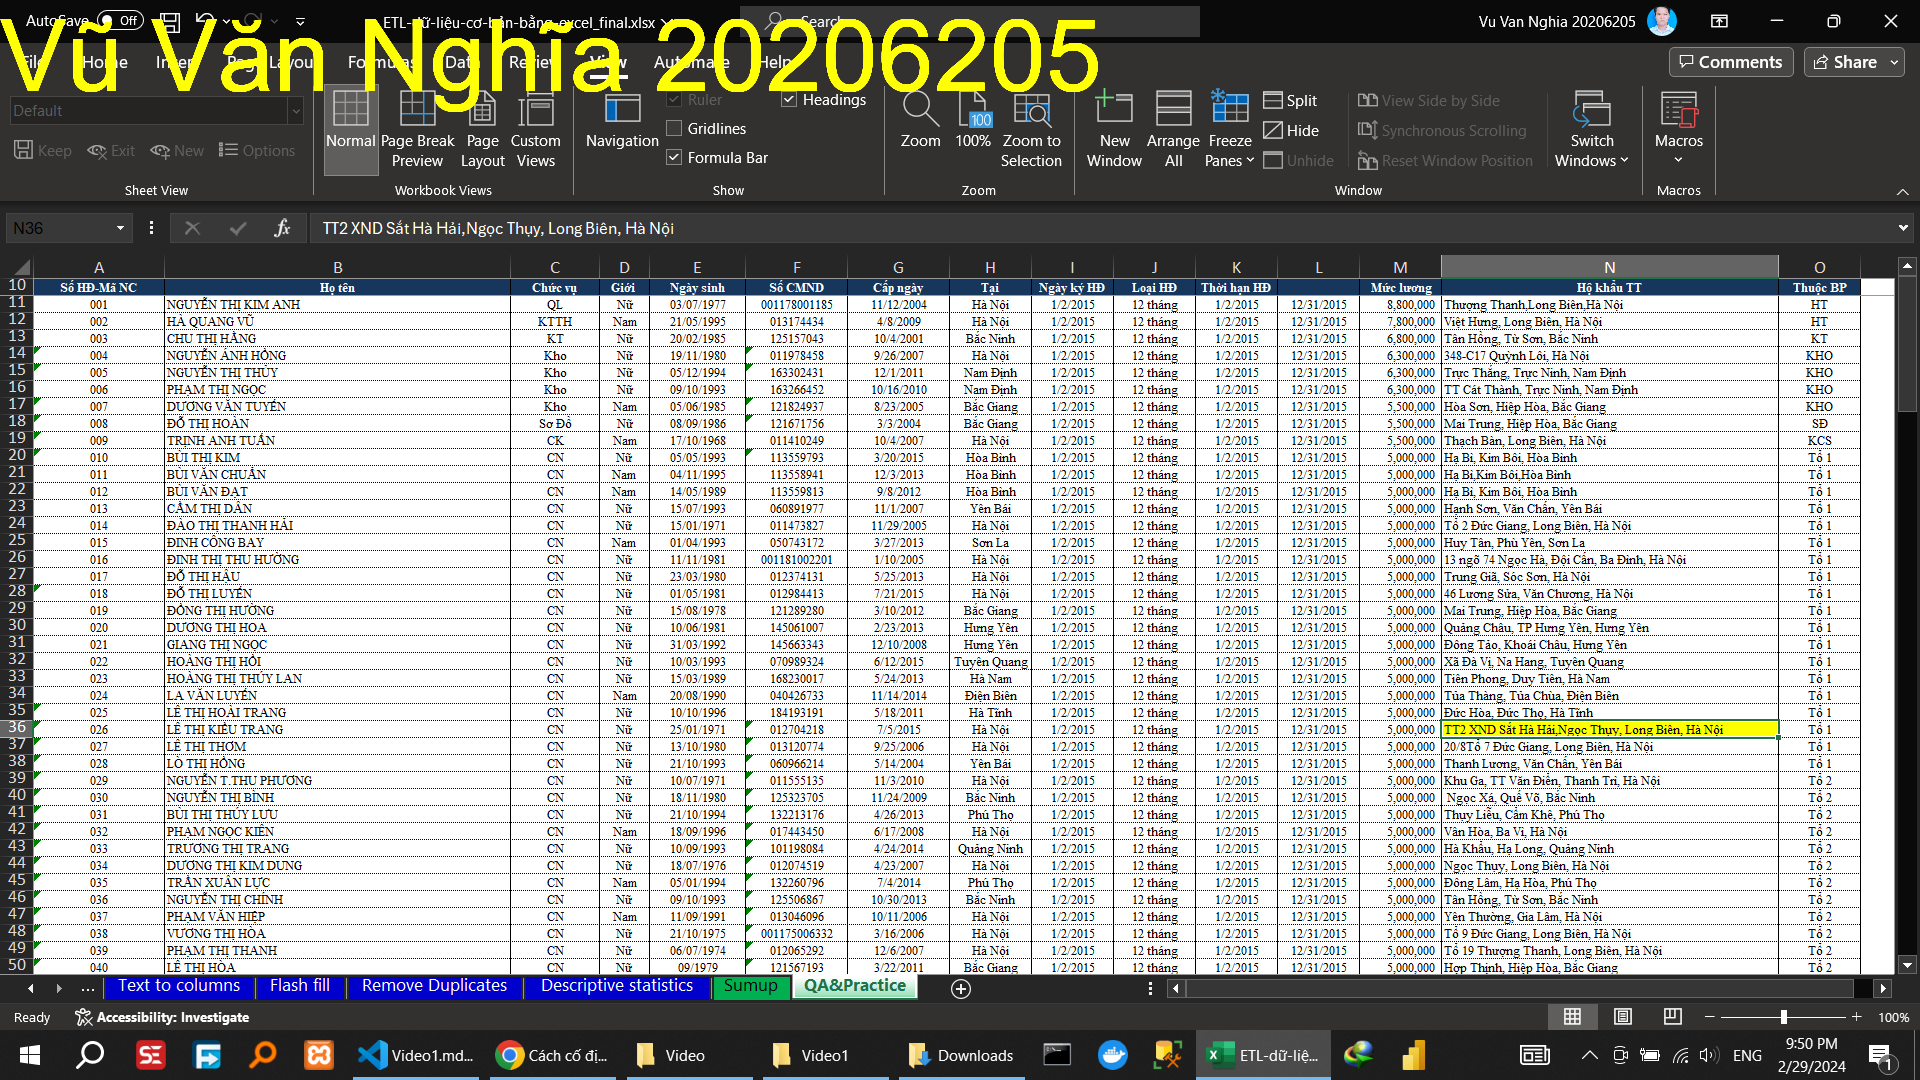
\includegraphics[scale = 0.15]{Video1/ThucHanh/2.png}
%     \caption{Thực hành đóng băng tiêu đề dữ liệu}
% \end{figure}

% % \paragraph{Thực hành tách họ và tên bằng công thức}
% % \subparagraph{Thực hành tách họ và tên bằng công thức}
% \begin{figure}[h]
%     \centering
%     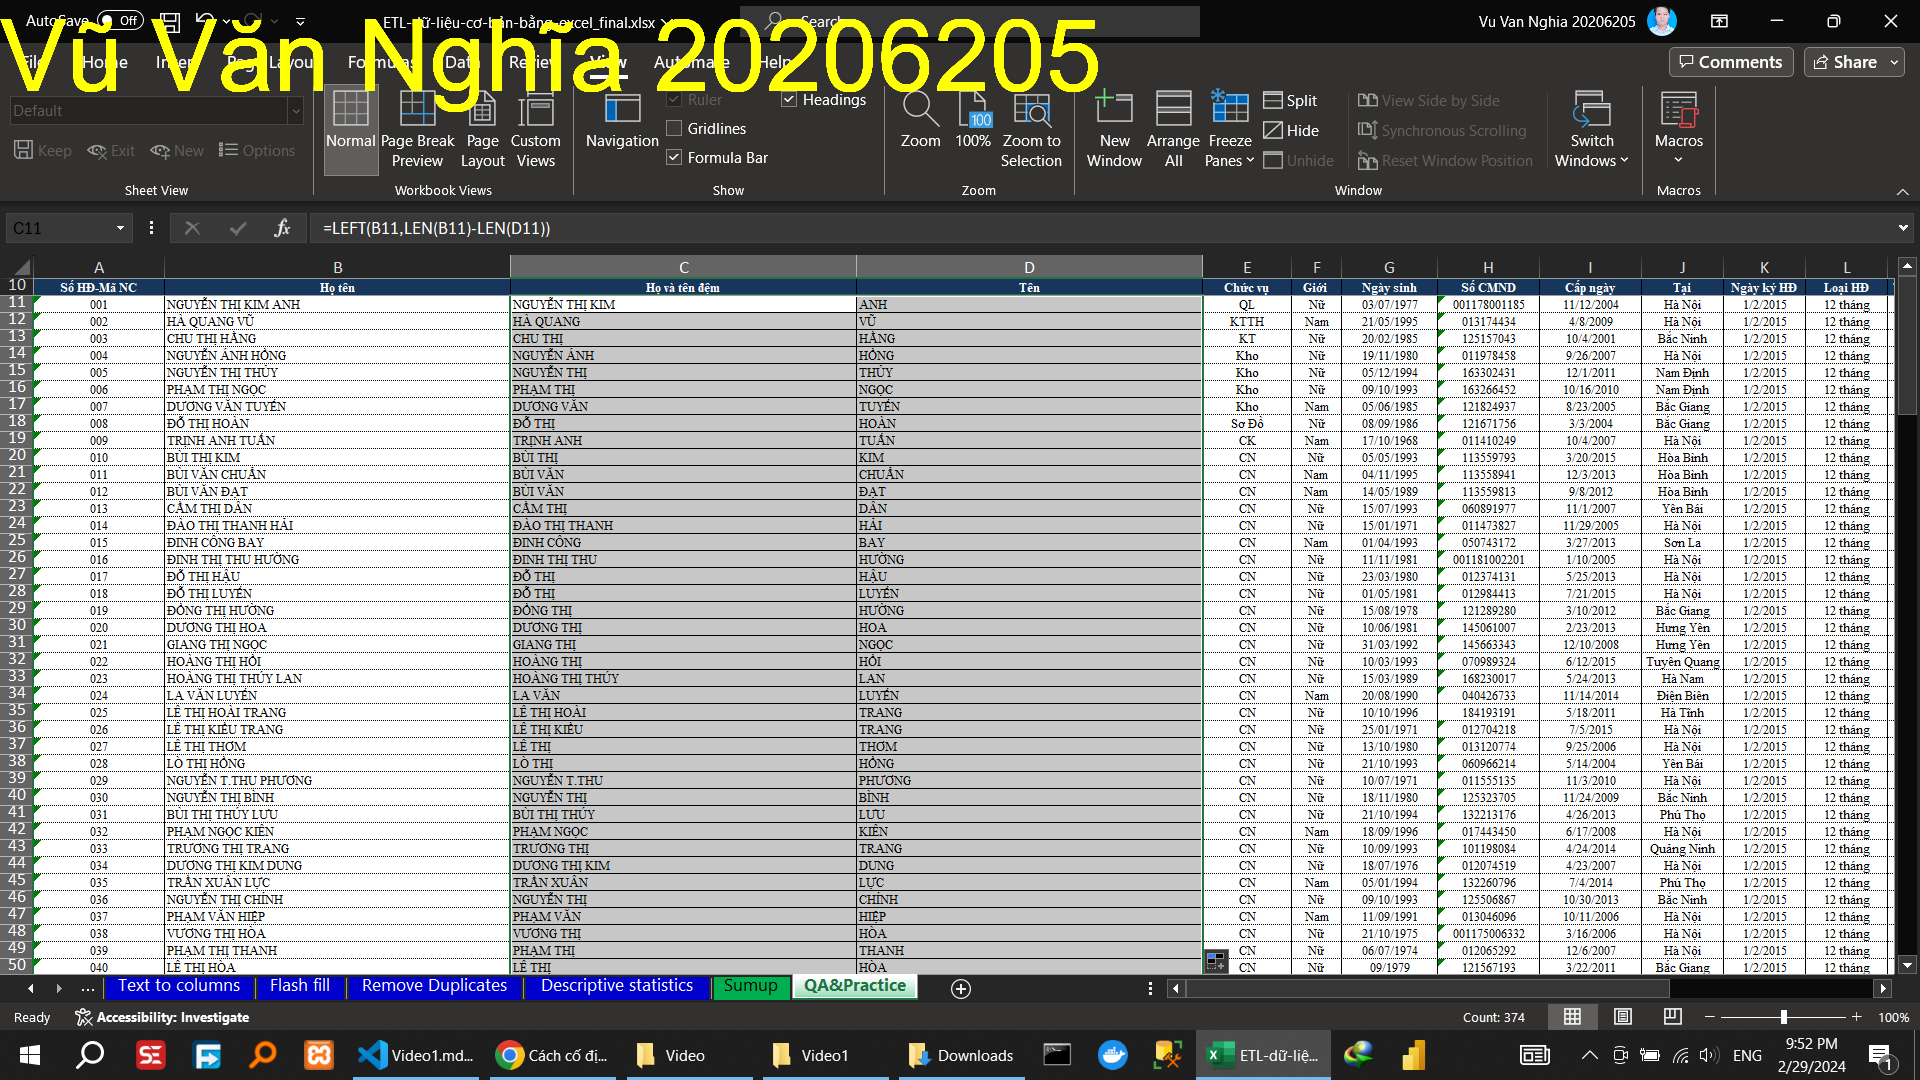
\includegraphics[scale = 0.15]{Video1/ThucHanh/3.png}
%     \caption{Thực hành tách họ và tên bằng công thức}
% \end{figure}

% % \paragraph{Thực hành tách họ và tên bằng flash fill}
% % \subparagraph{Thực hành tách họ và tên bằng flash fill}
% \begin{figure}[h]
%     \centering
%     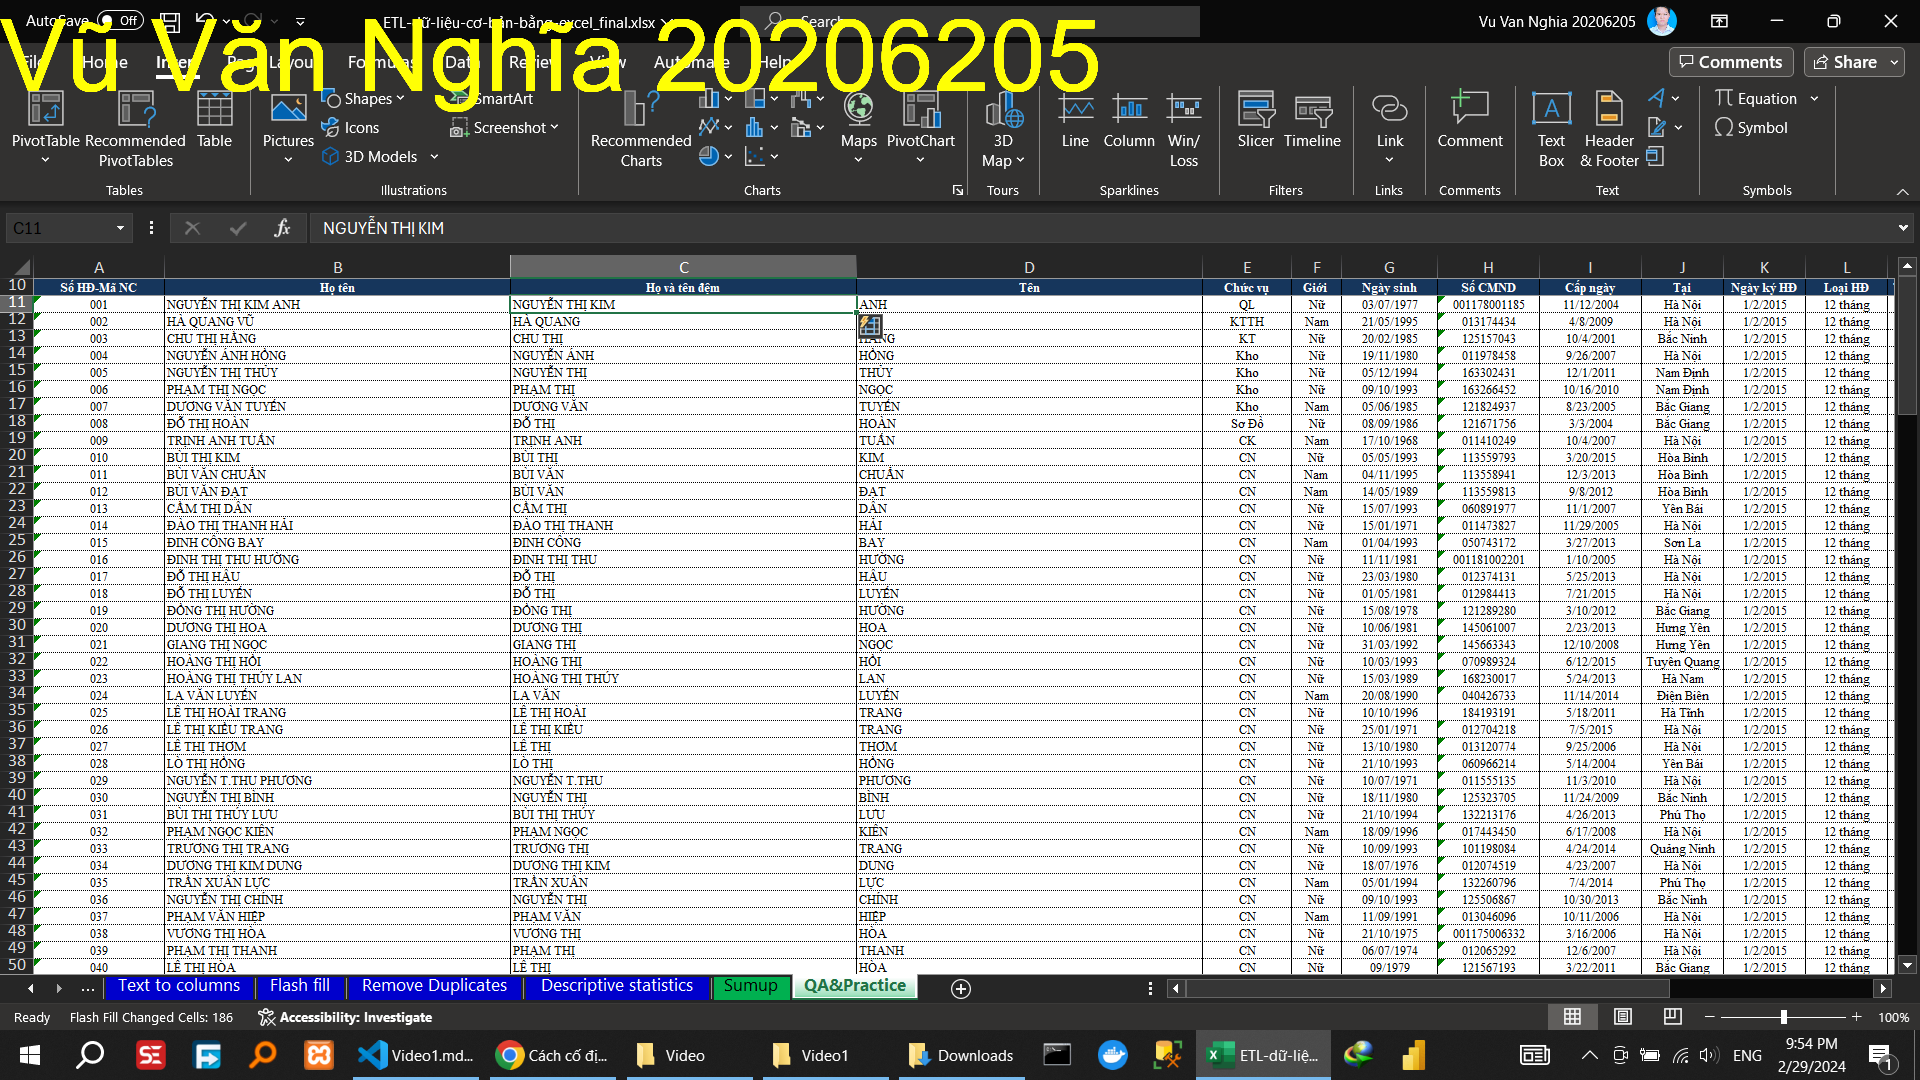
\includegraphics[scale = 0.15]{Video1/ThucHanh/4.png}
%     \caption{Thực hành tách họ và tên bằng flash fill}
% \end{figure}

% % \paragraph{Thực hành sắp xếp danh sách theo tên nhân công}
% % \subparagraph{Thực hành sắp xếp danh sách theo tên nhân công}
% \begin{figure}[h]
%     \centering
%     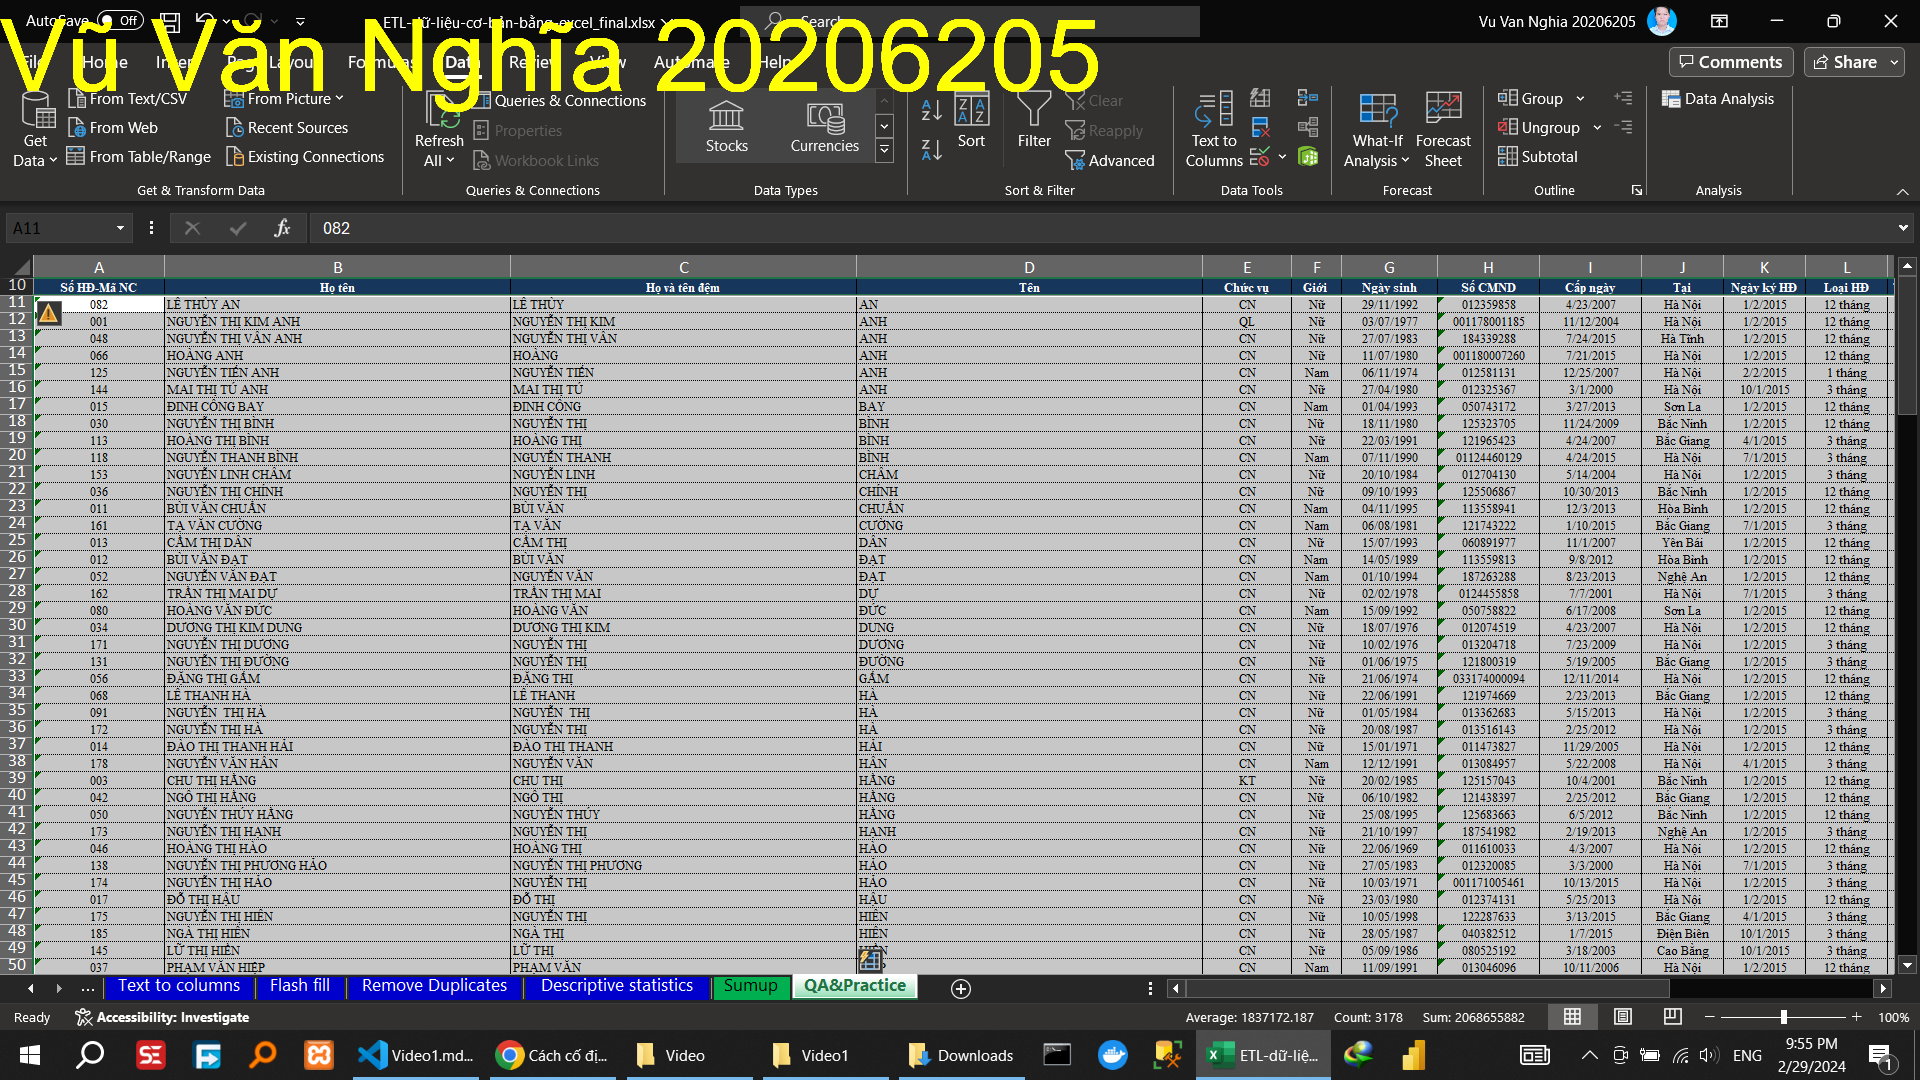
\includegraphics[scale = 0.15]{Video1/ThucHanh/5.png}
%     \caption{Thực hành sắp xếp danh sách theo tên nhân công}
% \end{figure}

% % <!-- Lập danh các chức vụ của mỗi bộ phận ( Remove Duplicates) -->
% % \paragraph{Thực hành lập danh sách các chức vụ của mỗi bộ phận}
% % \subparagraph{Thực hành lập danh sách các chức vụ của mỗi bộ phận}
% \begin{figure}[h]
%     \centering
%     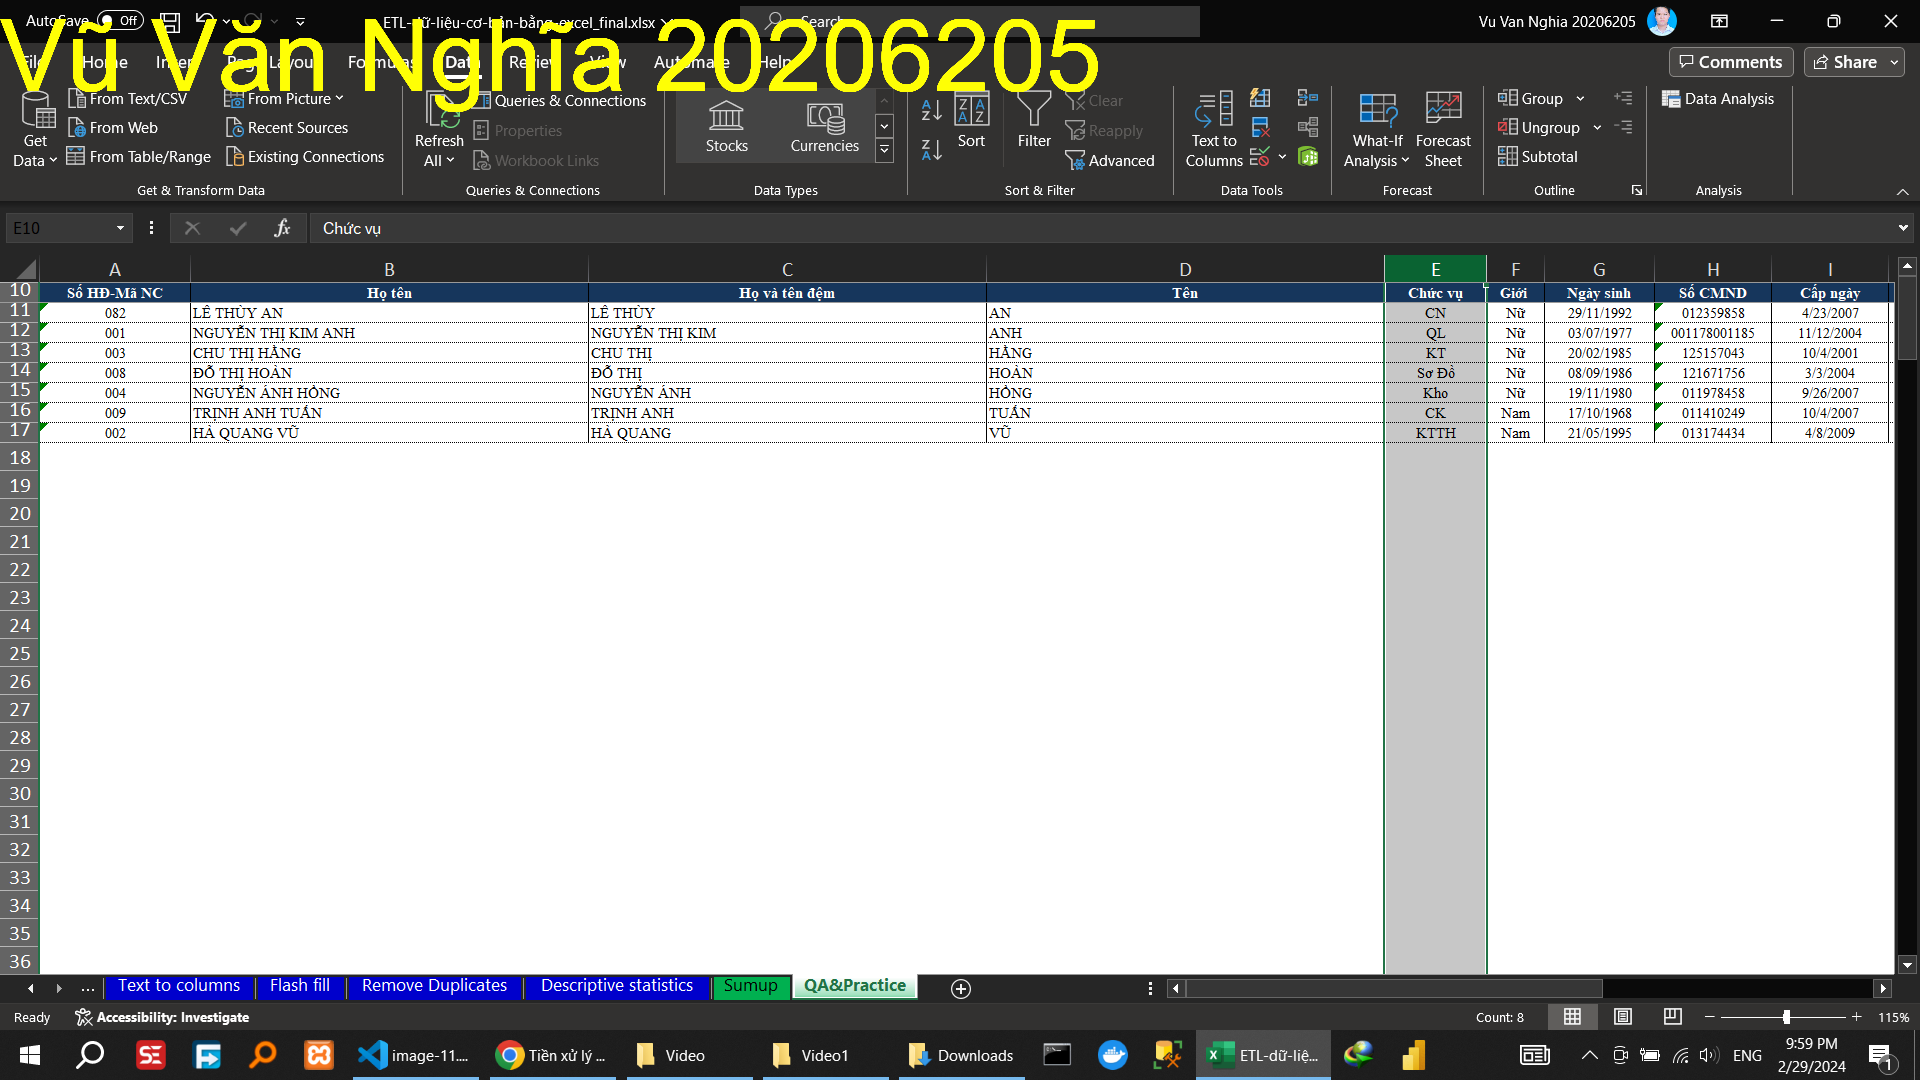
\includegraphics[scale = 0.15]{Video1/ThucHanh/6.png}
%     \caption{Thực hành lập danh sách các chức vụ của mỗi bộ phận}
% \end{figure}

% % \newpage
% % \subsection{Video 2}
% % \subsubsection{Hướng dẫn}
% \begin{figure}[h]
%     \centering
%     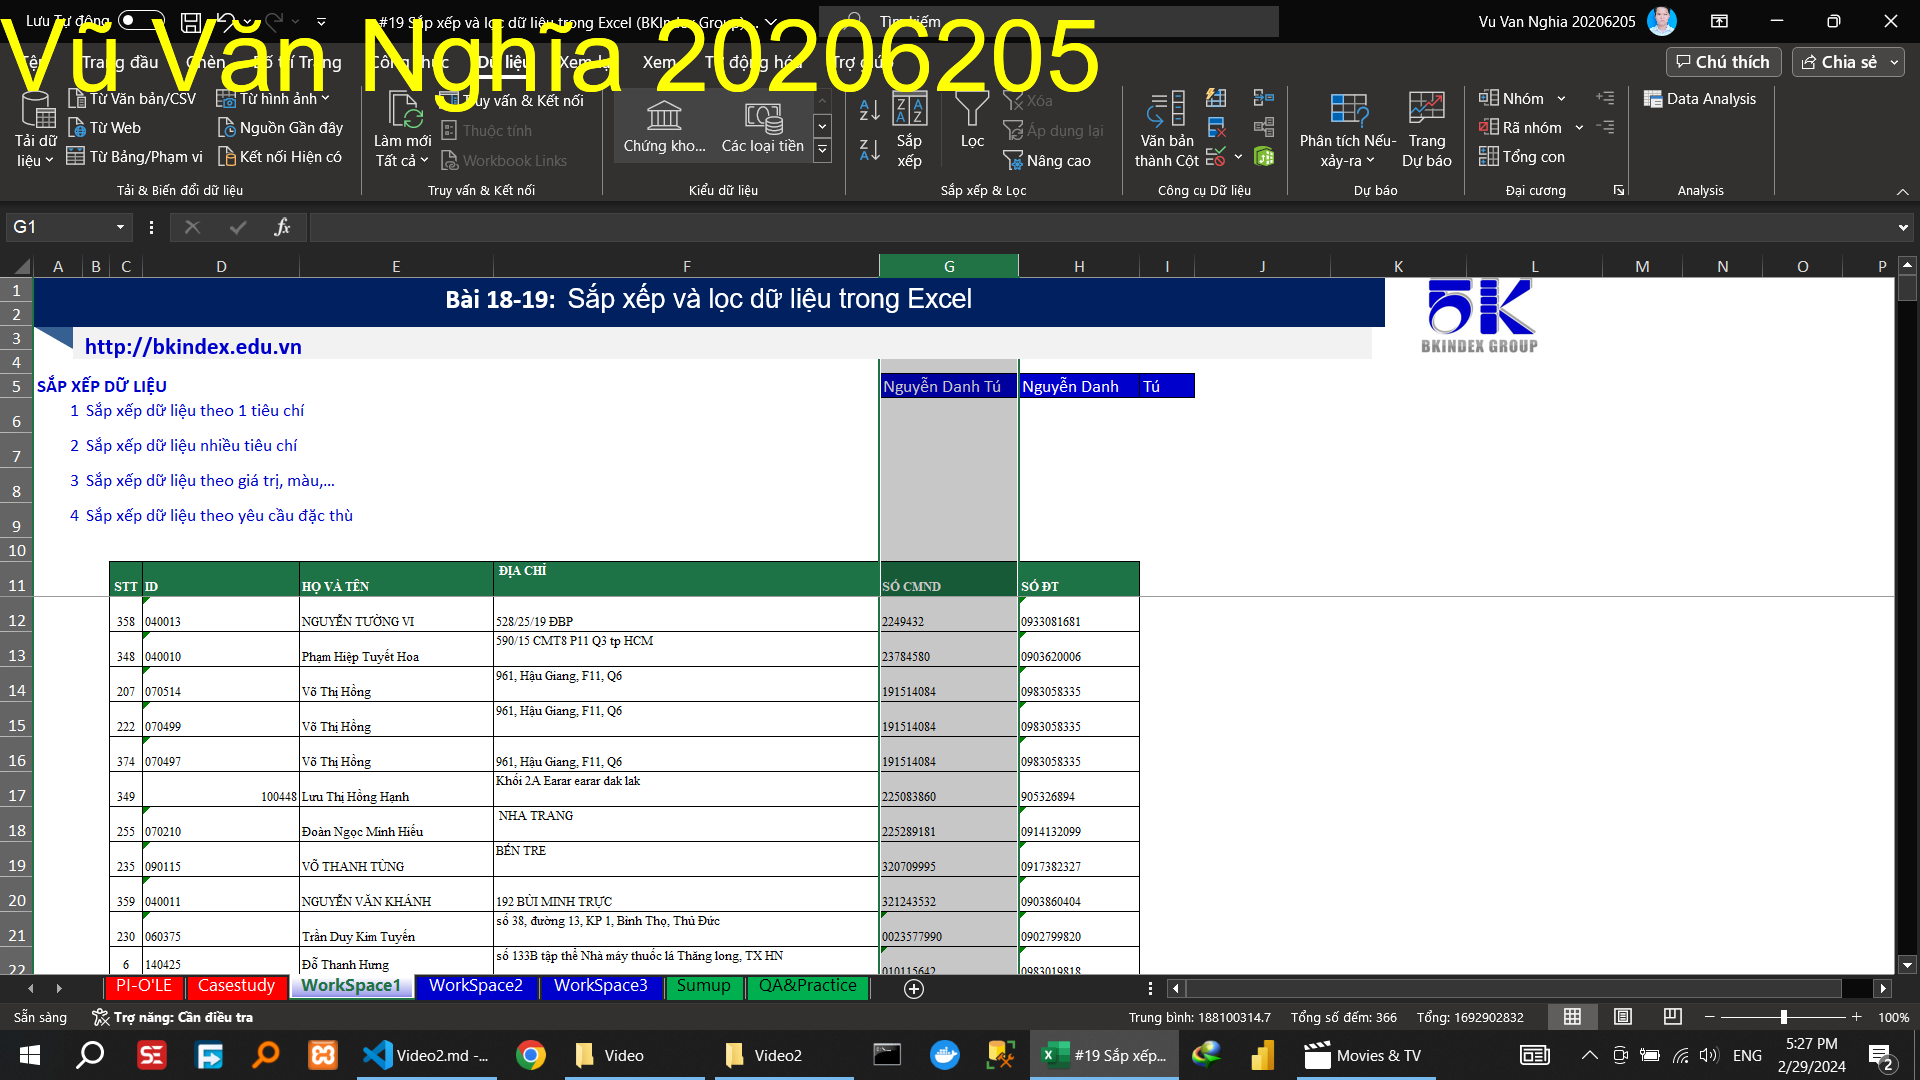
\includegraphics[scale = 0.15]{Video2/HuongDan/0.png}
%     \caption{Hướng dẫn sắp xếp dữ liệu theo 1 tiêu chí là số CMND}
% \end{figure}

% \begin{figure}[h]
%     \centering
%     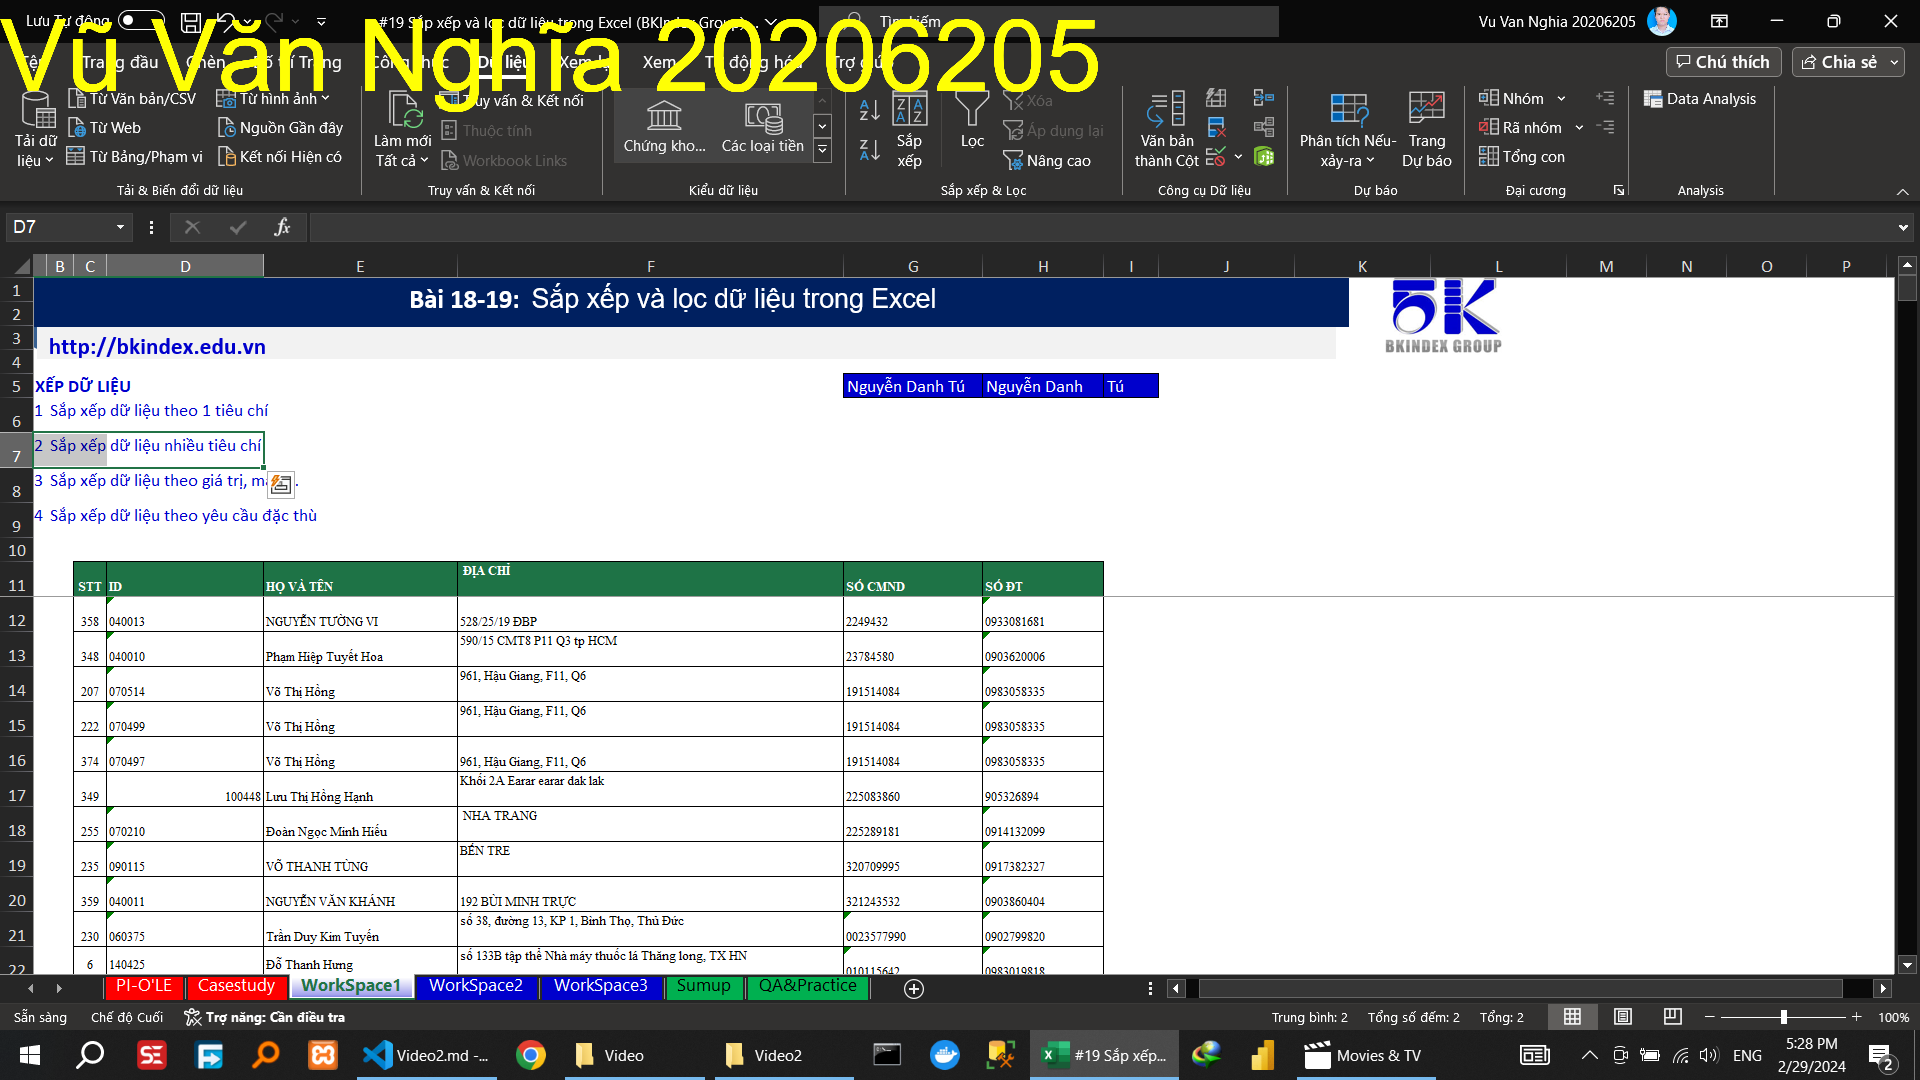
\includegraphics[scale = 0.15]{Video2/HuongDan/1.png}
%     \caption{Hướng dẫn sắp xếp dữ liệu theo nhiều tiêu chí số CMND và số điện thoại}
% \end{figure}

% \begin{figure}[h]
%     \centering
%     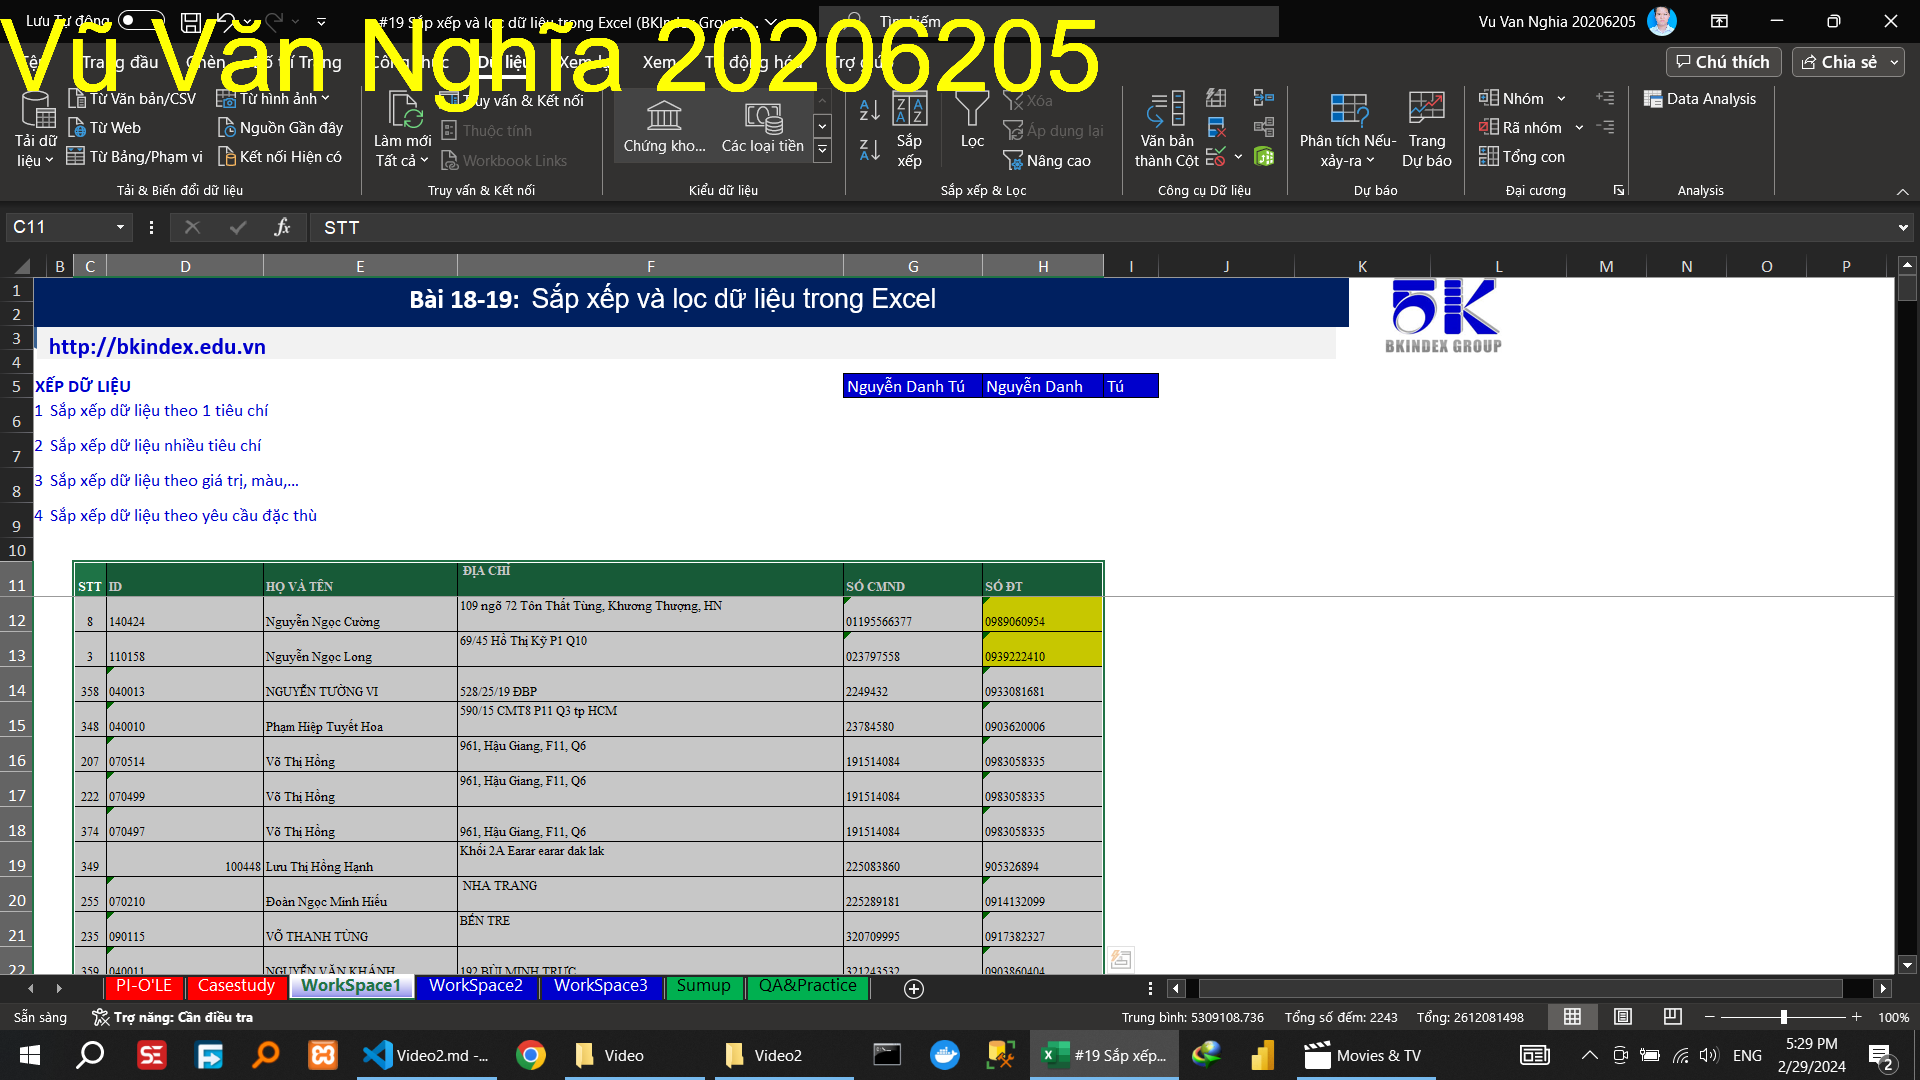
\includegraphics[scale = 0.15]{Video2/HuongDan/2.png}
%     \caption{Hướng dẫn sắp xếp dữ liệu theo giá trị, màu,\dots của số điện thoại}
% \end{figure}

% \begin{figure}[h]
%     \centering
%     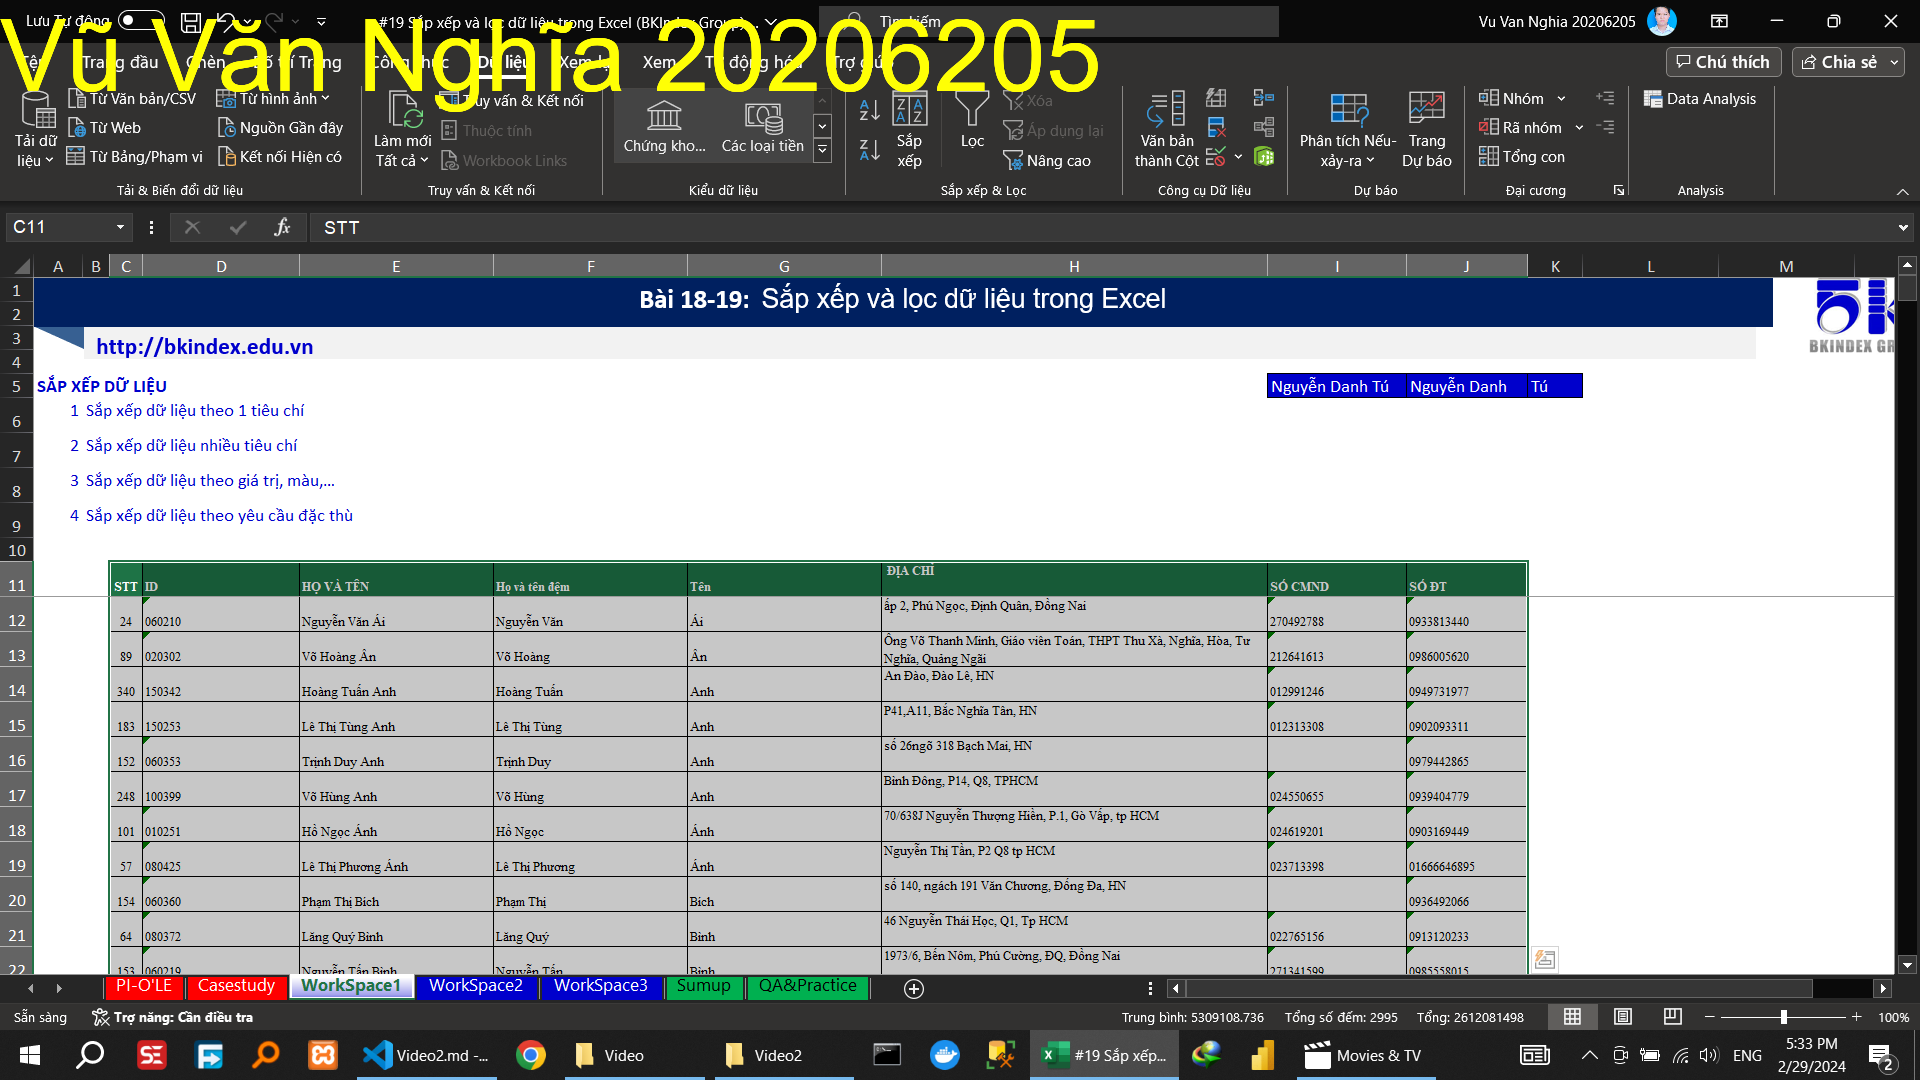
\includegraphics[scale = 0.15]{Video2/HuongDan/3.png}
%     \caption{Hướng dẫn sắp xếp dữ liệu theo yêu cầu đặc thù là tên và tên đệm}
% \end{figure}

% \begin{figure}[h]
%     \centering
%     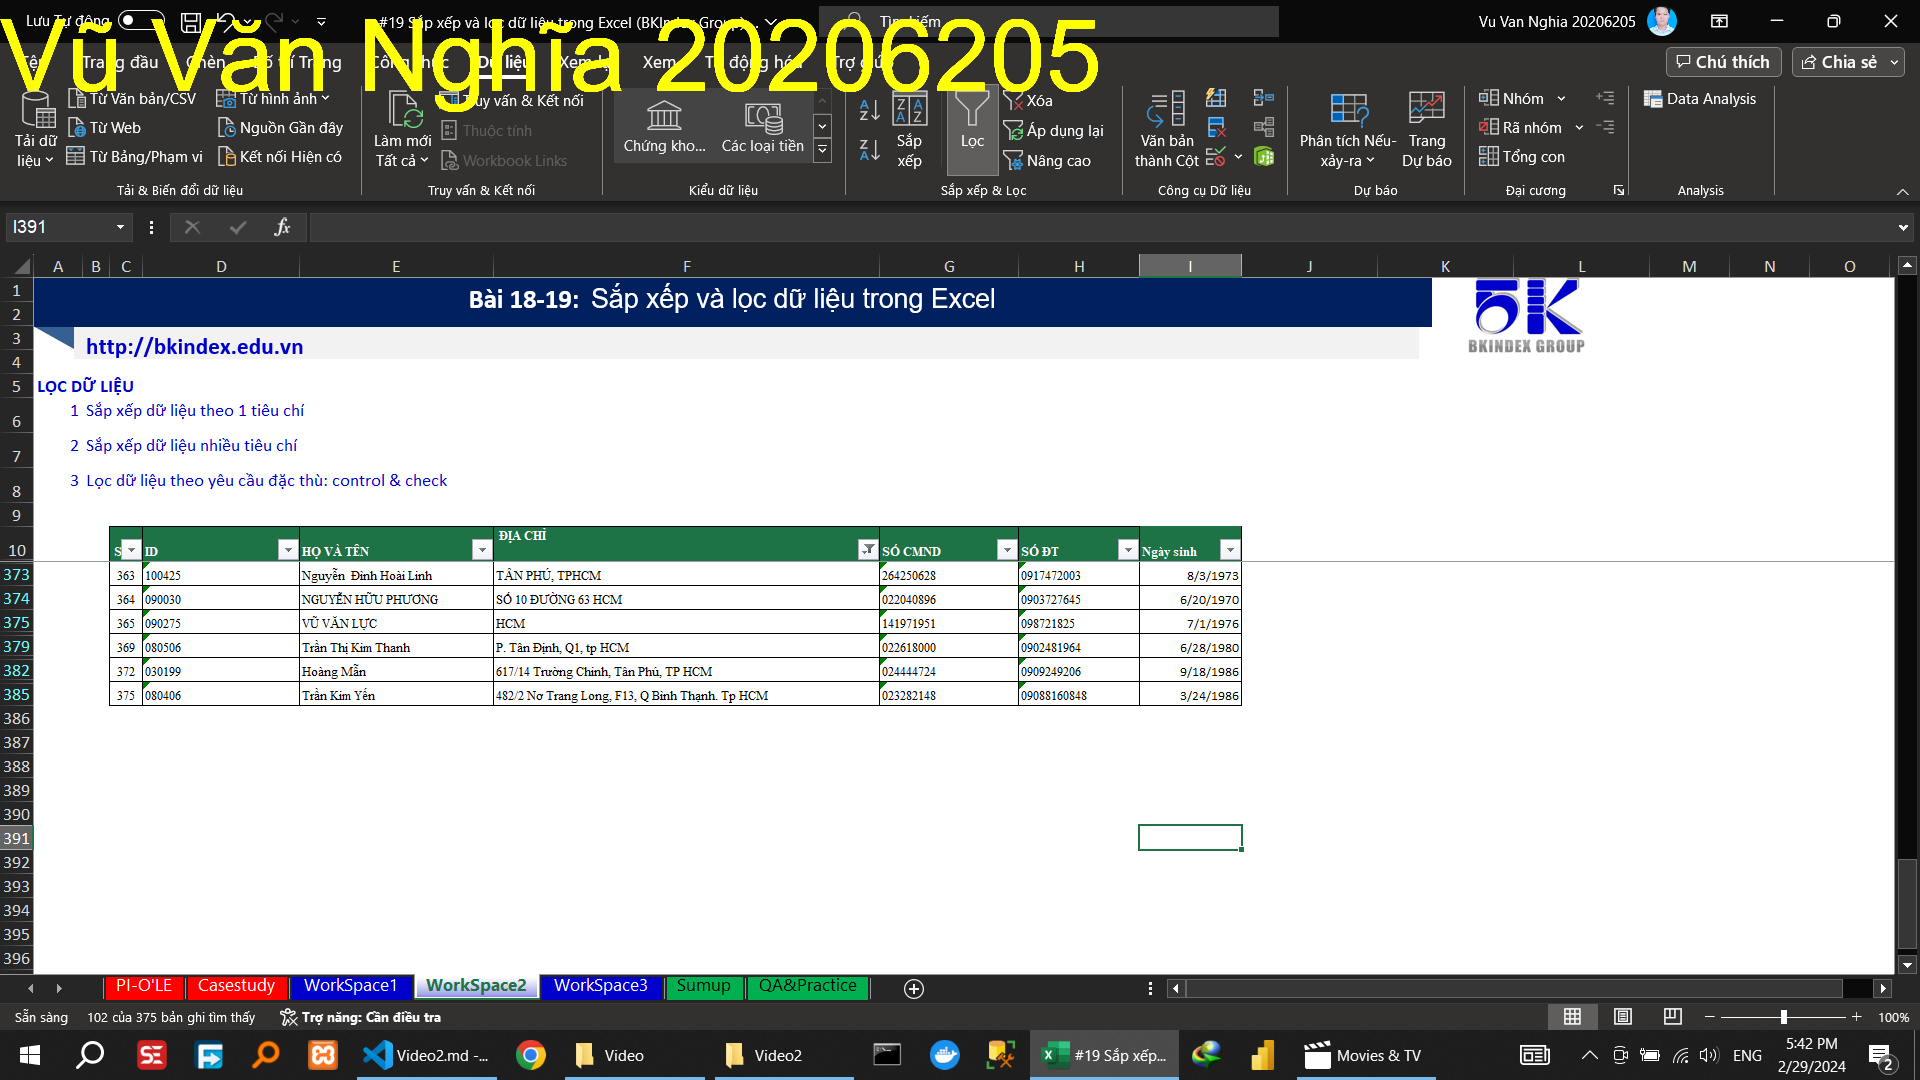
\includegraphics[scale = 0.15]{Video2/HuongDan/4.png}
%     \caption{Hướng dẫn lọc dữ liệu theo 1 tiêu chí là địa chỉ HCM}
% \end{figure}

% \begin{figure}[h]
%     \centering
%     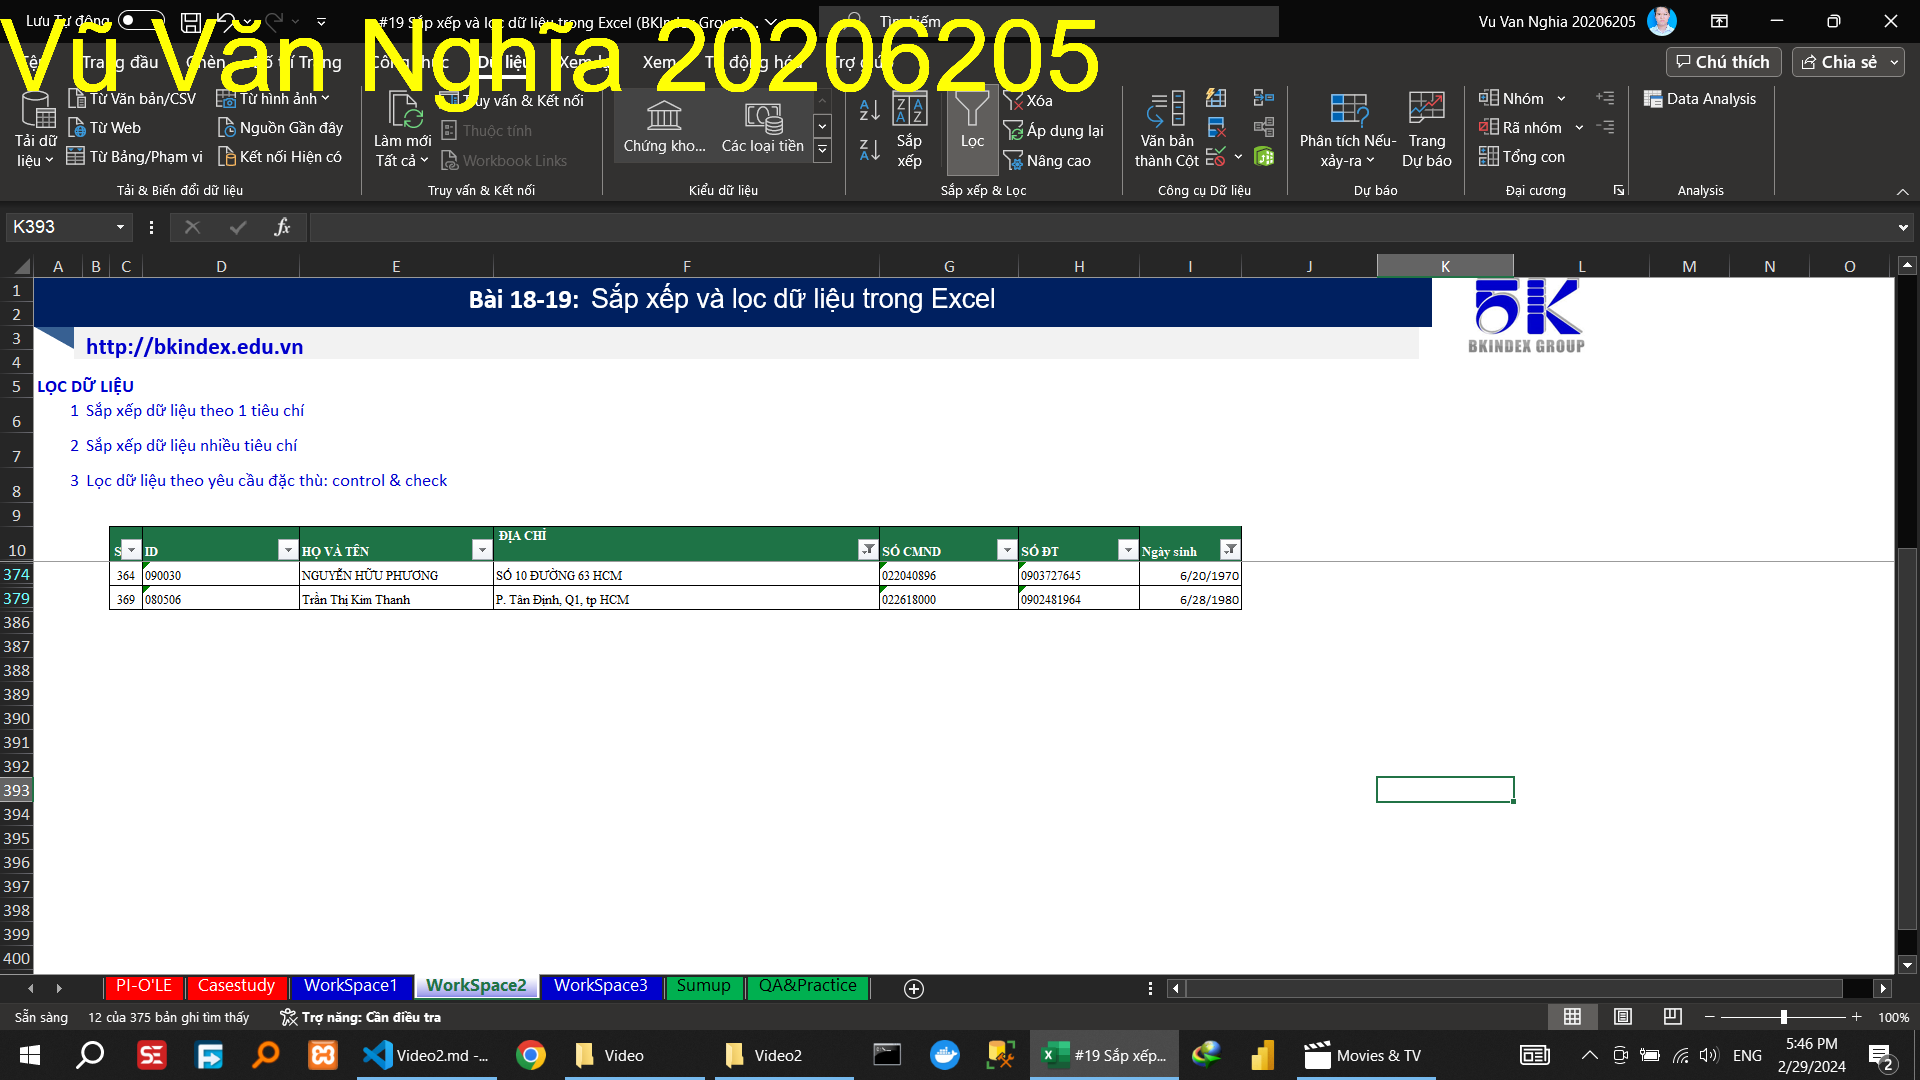
\includegraphics[scale = 0.15]{Video2/HuongDan/5.png}
%     \caption{Hướng dẫn lọc dữ liệu theo nhiều tiêu chí là sinh tháng 6 và ở HCM}
% \end{figure}

% \begin{figure}[h]
%     \centering
%     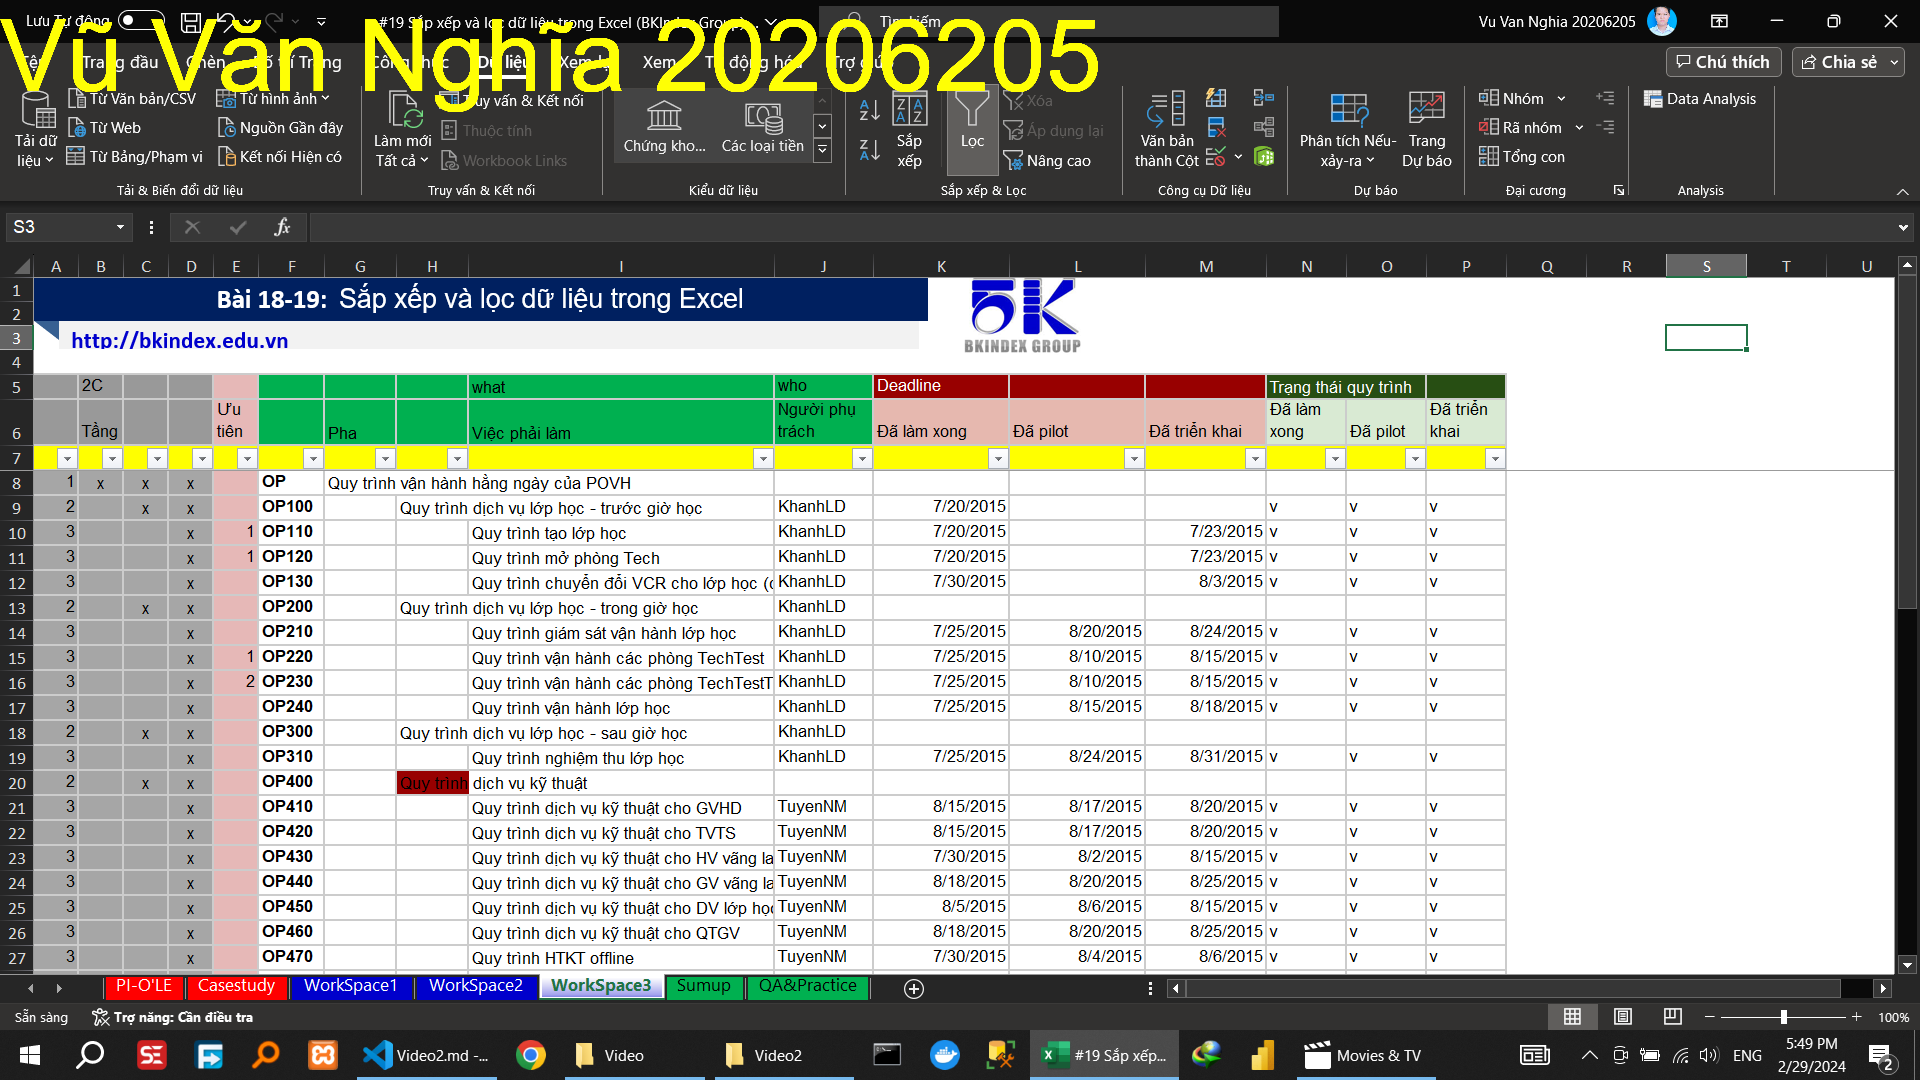
\includegraphics[scale = 0.15]{Video2/HuongDan/6.png}
%     \caption{Hướng dẫn lọc dữ liệu theo yêu cầu đặc thù: control và check}
% \end{figure}

% % \subsubsection{Thực hành}
% \begin{figure}[h]
%     \centering
%     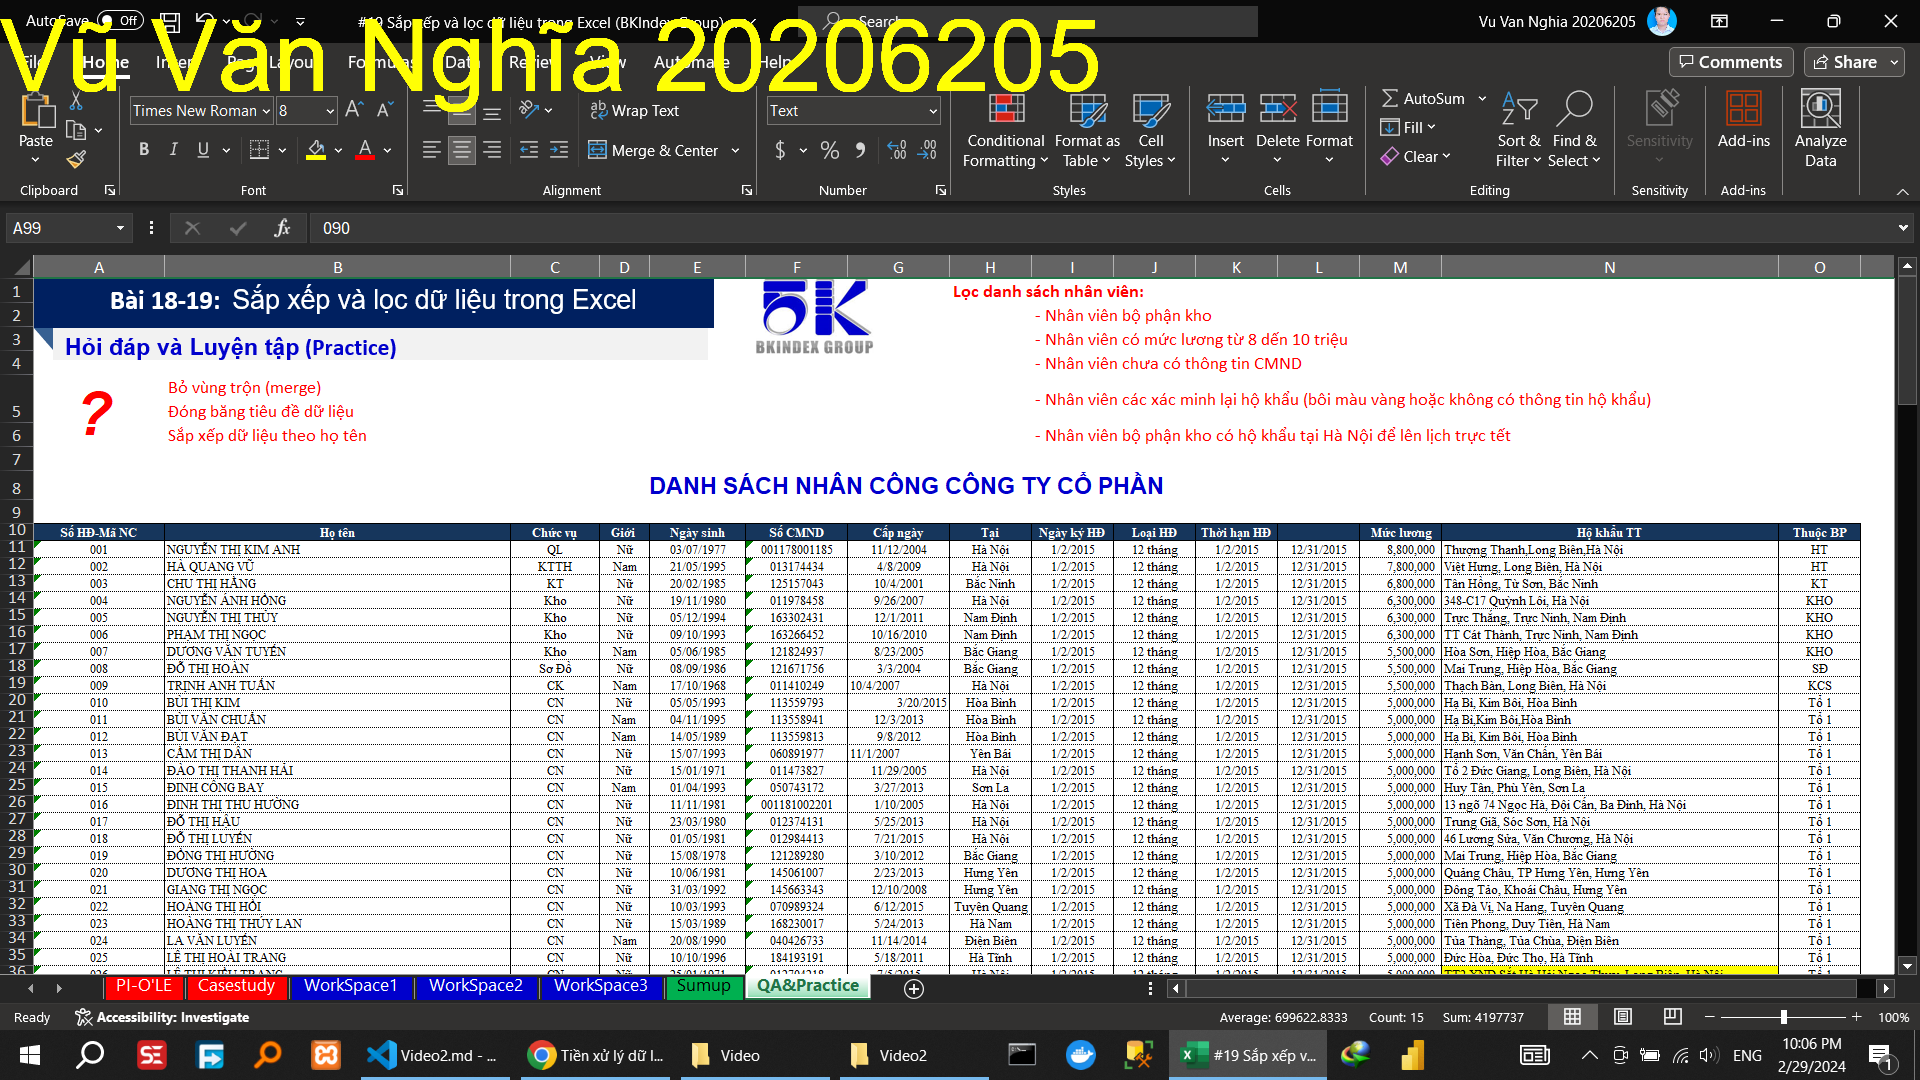
\includegraphics[scale = 0.15]{Video2/ThucHanh/0.png}
%     \caption{Thực hành bỏ vùng trộn (merge)}
% \end{figure}

% \begin{figure}[h]
%     \centering
%     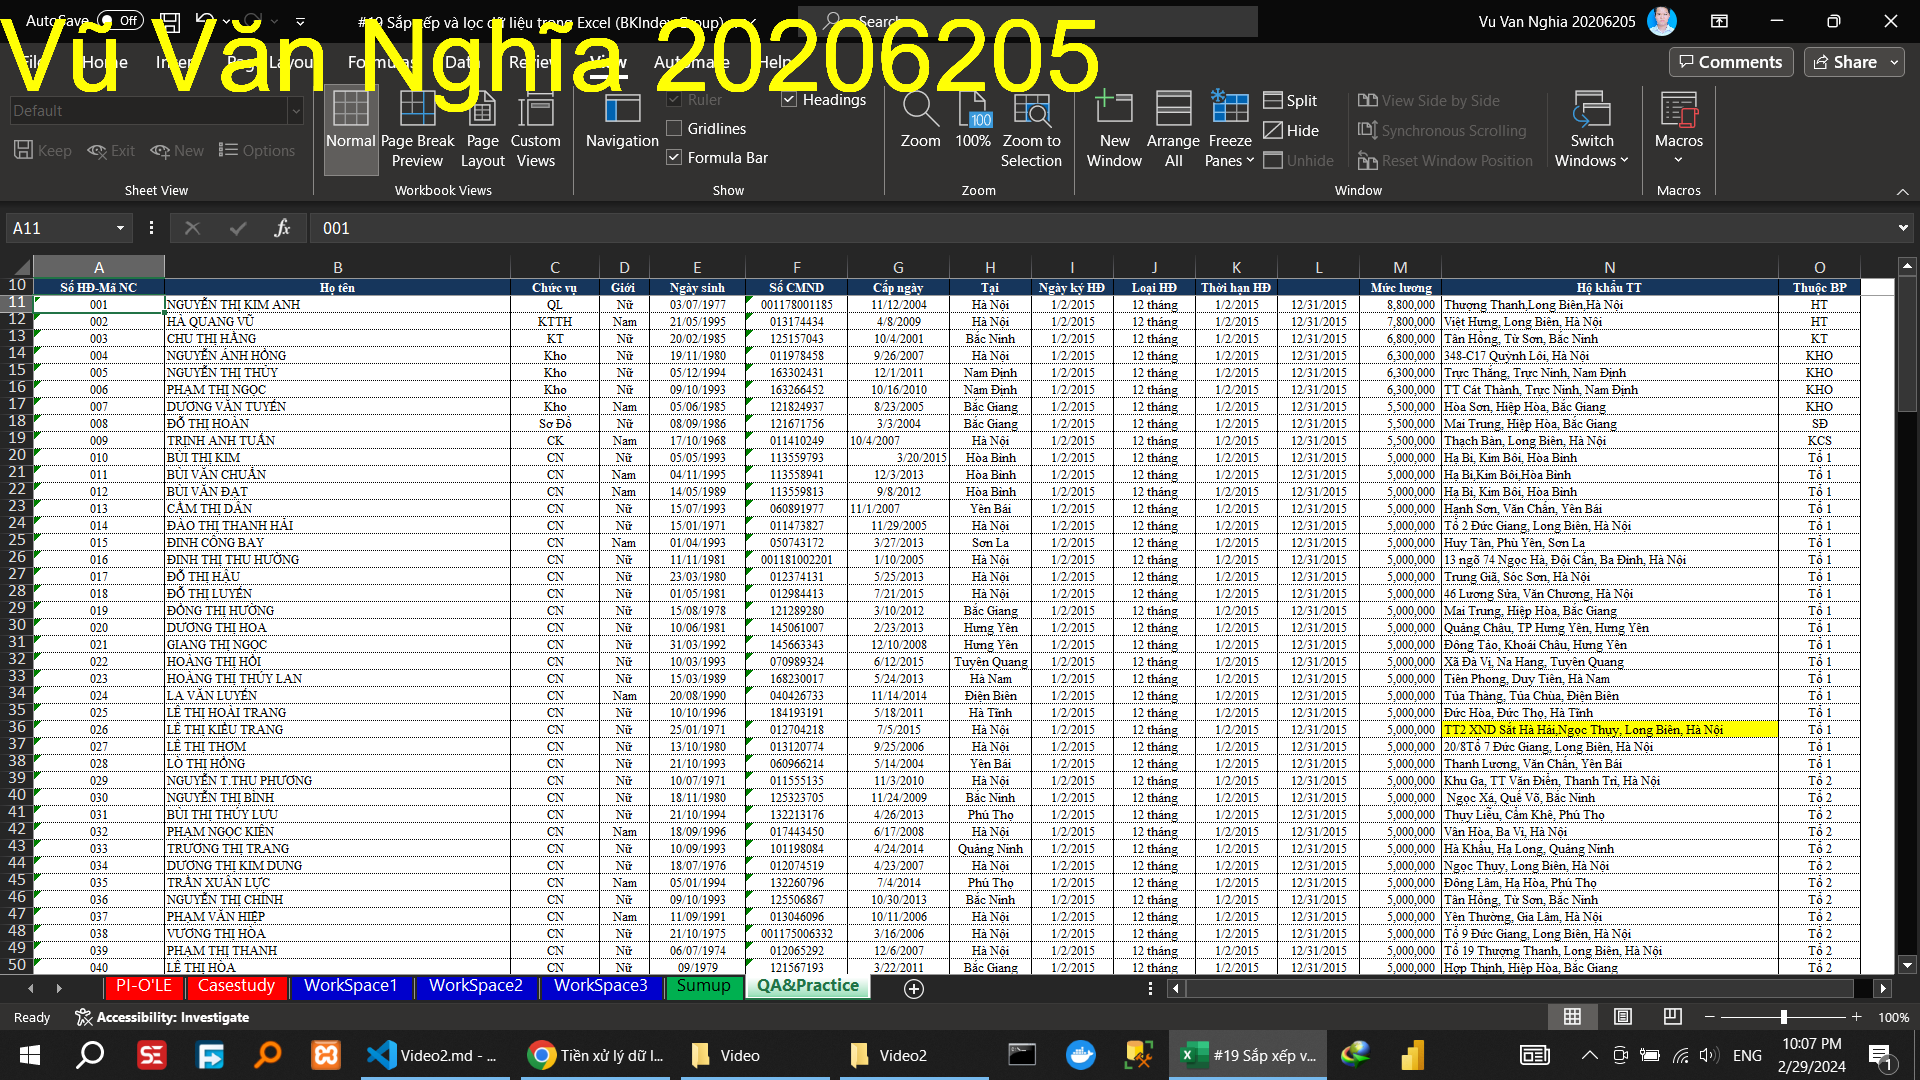
\includegraphics[scale = 0.15]{Video2/ThucHanh/1.png}
%     \caption{Thực hành đóng băng tiêu đề dữ liệu}
% \end{figure}

% \begin{figure}[h]
%     \centering
%     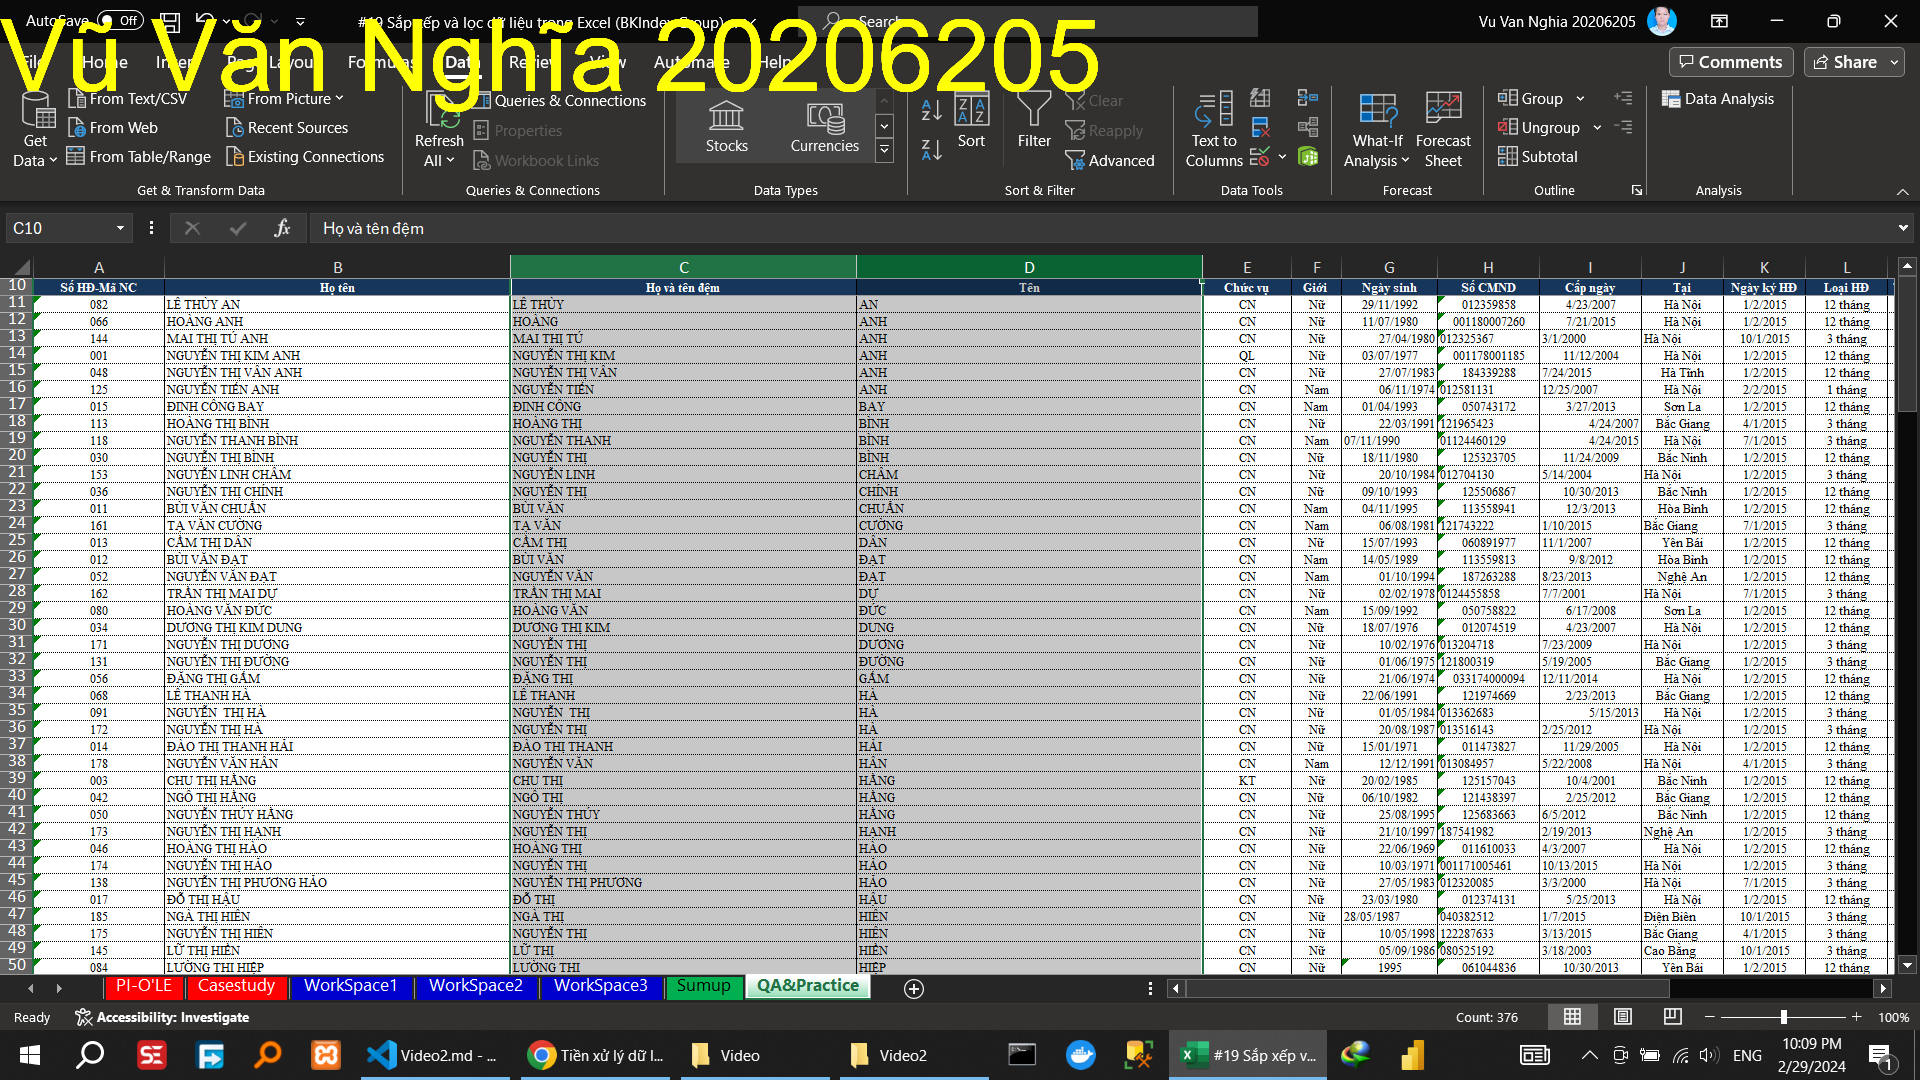
\includegraphics[scale = 0.15]{Video2/ThucHanh/2.png}
%     \caption{Thực hành sắp xếp dữ liệu theo họ tên}
% \end{figure}

% \begin{figure}[h]
%     \centering
%     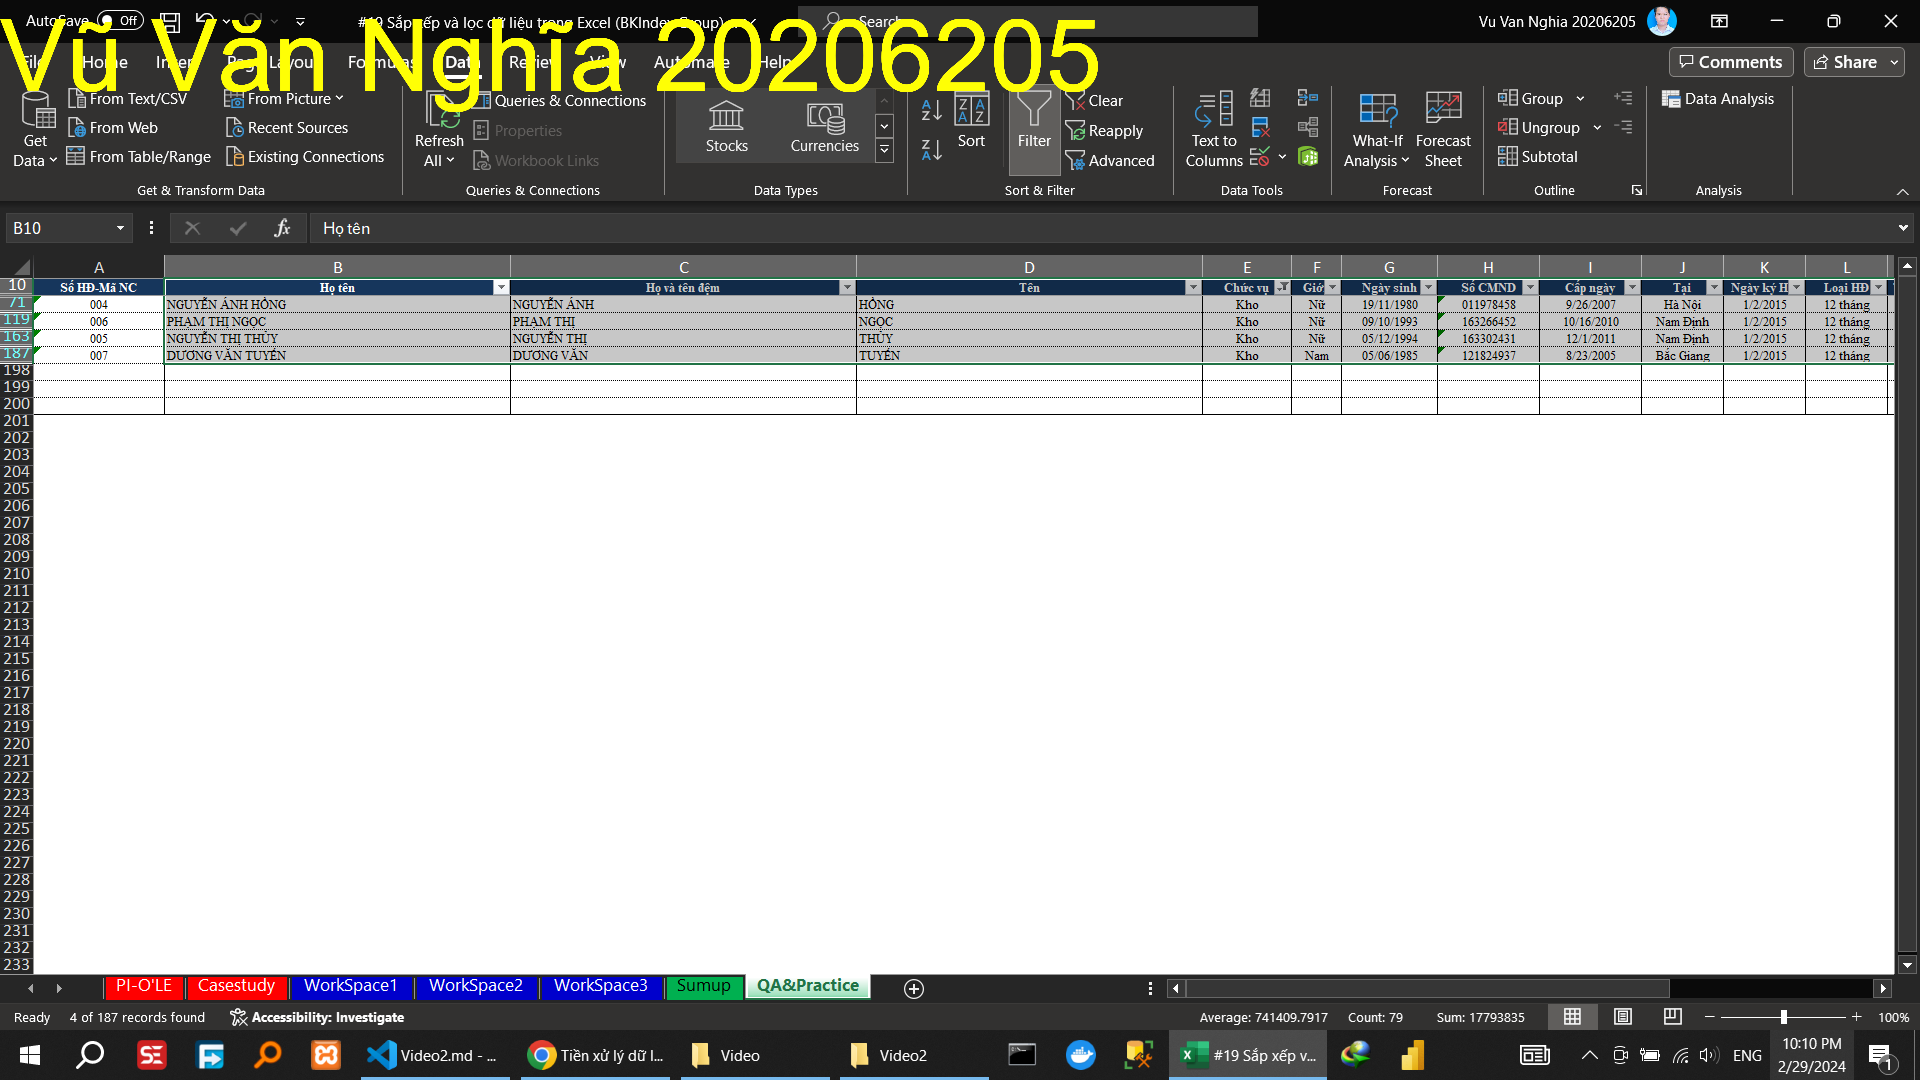
\includegraphics[scale = 0.15]{Video2/ThucHanh/3.png}
%     \caption{Thực hành lọc danh sách nhân viên bộ phận kho}
% \end{figure}

% \begin{figure}[h]
%     \centering
%     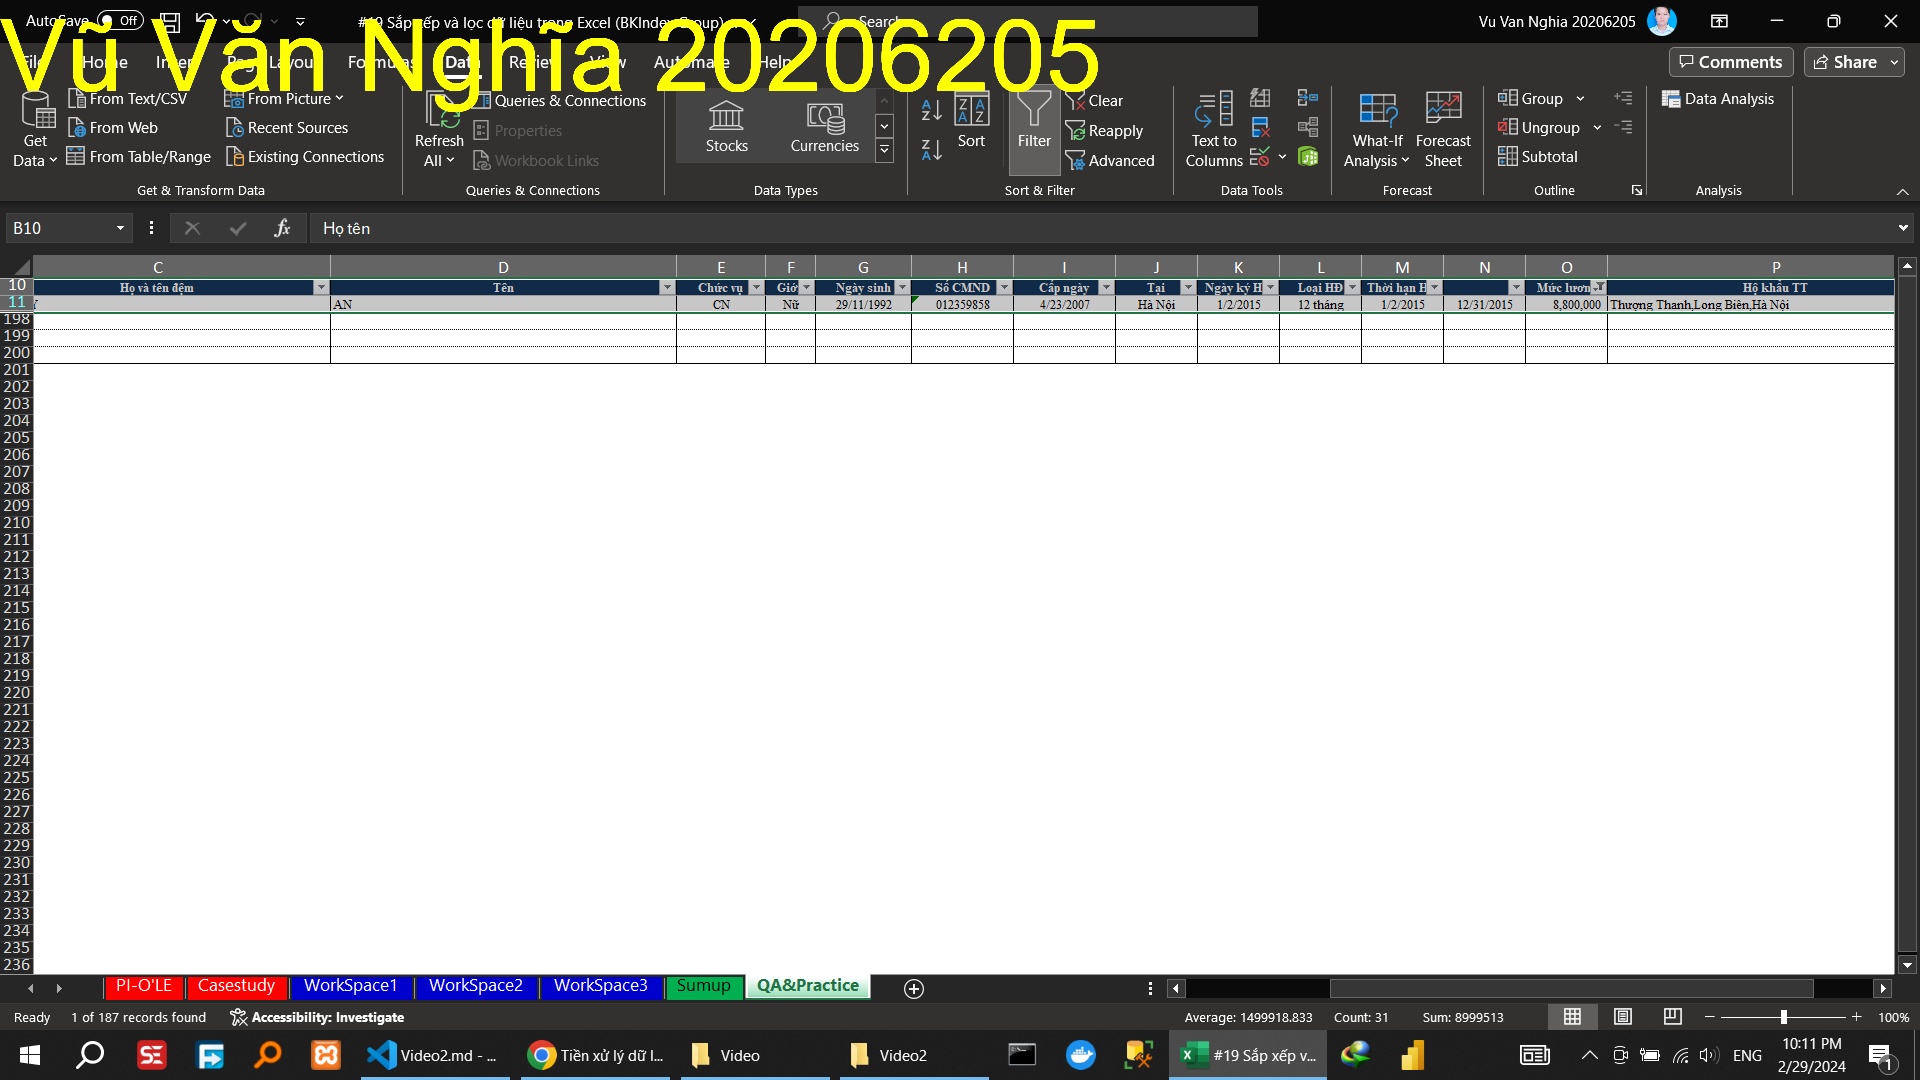
\includegraphics[scale = 0.15]{Video2/ThucHanh/4.png}
%     \caption{Thực hành lọc danh sách nhân viên có mức lương từ 8 đến 10 triệu}
% \end{figure}

% \begin{figure}[h]
%     \centering
%     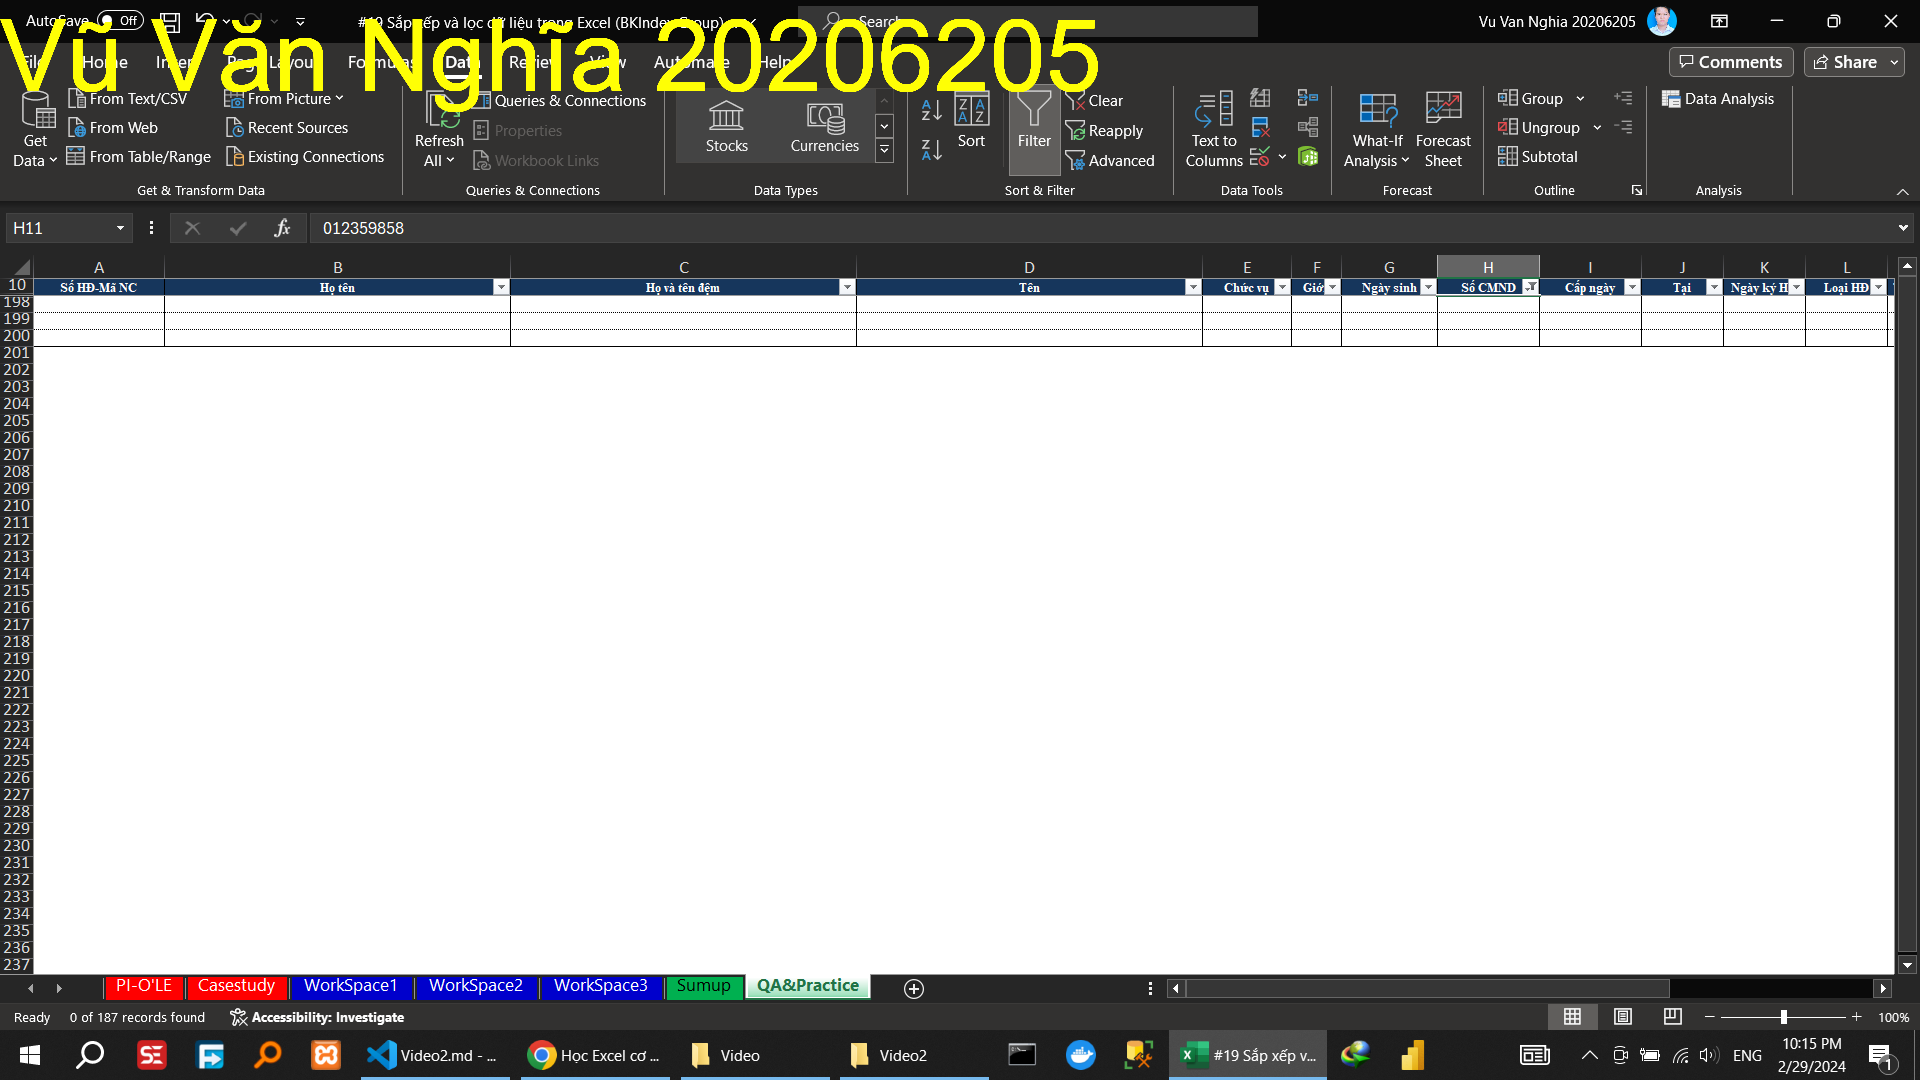
\includegraphics[scale = 0.15]{Video2/ThucHanh/5.png}
%     \caption{Thực hành lọc danh sách nhân viên chưa có thông tin CMND}
% \end{figure}

% \begin{figure}[h]
%     \centering
%     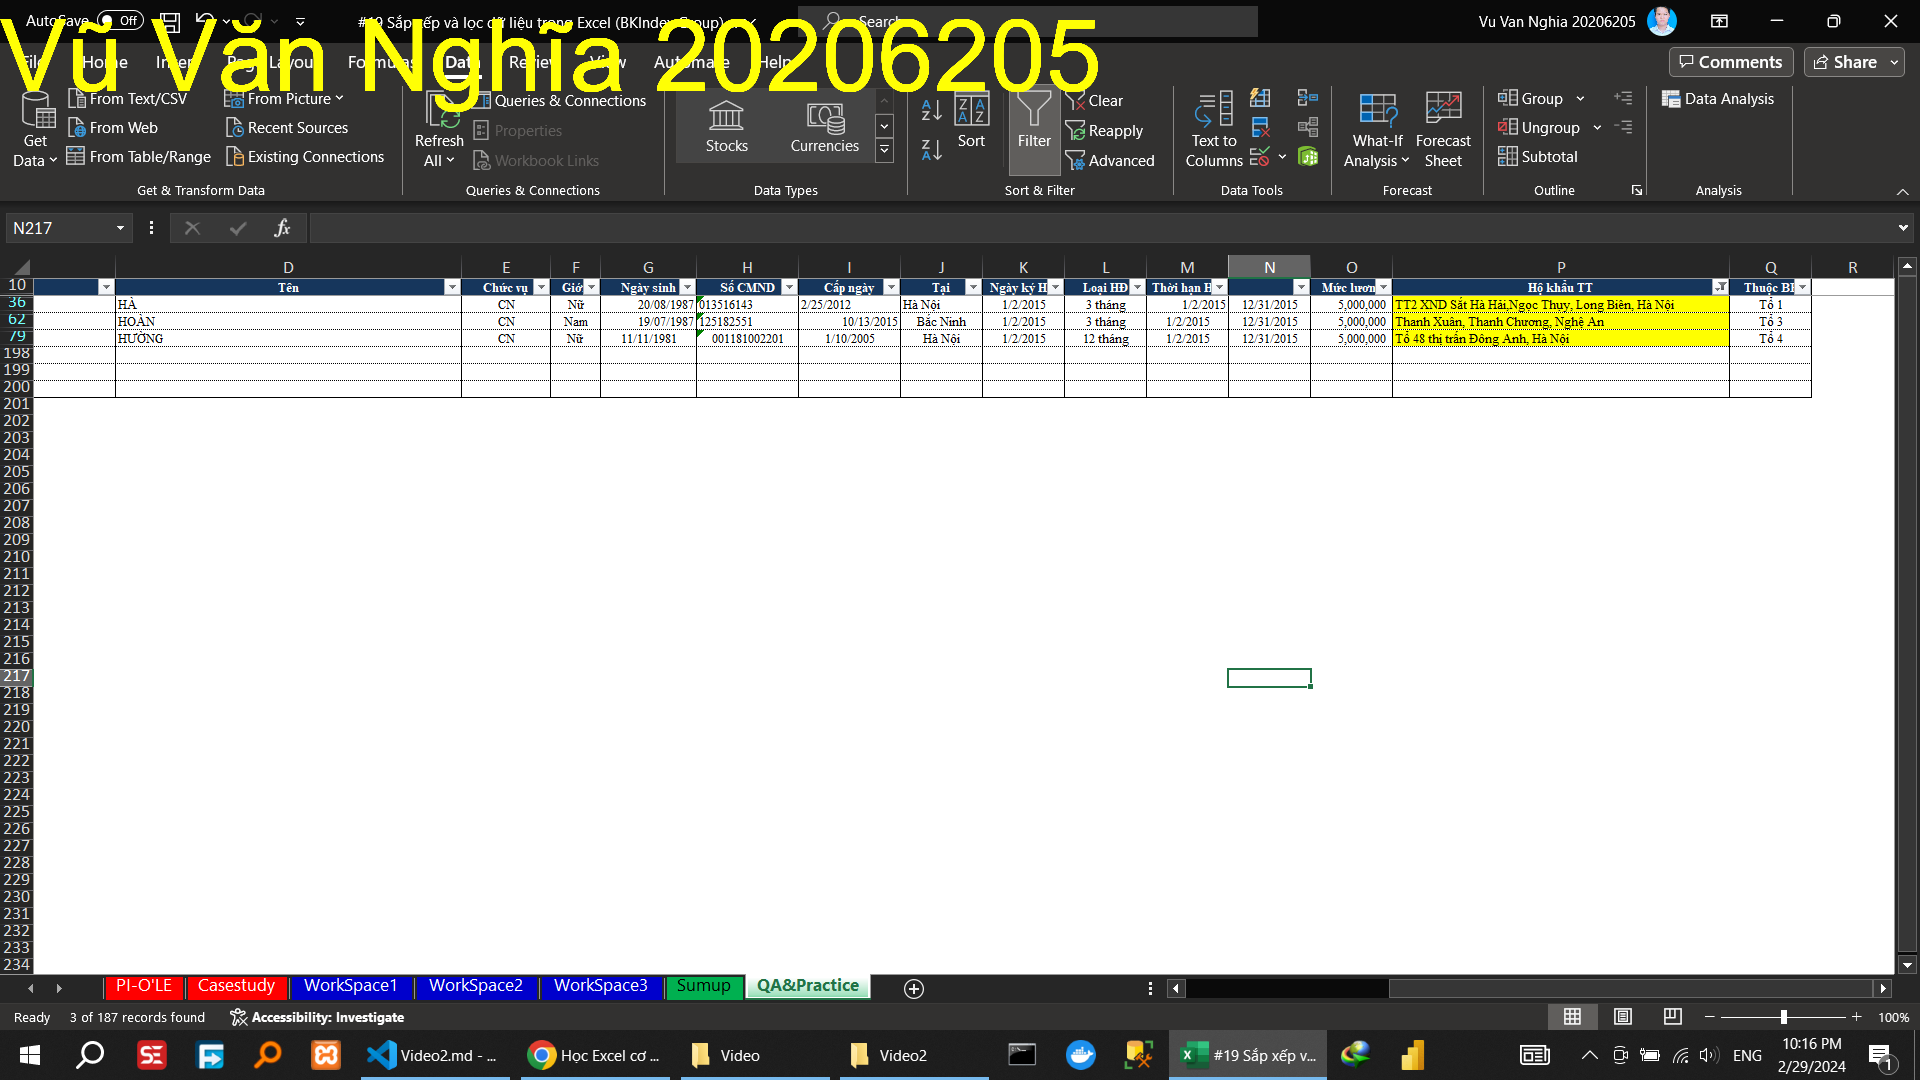
\includegraphics[scale = 0.15]{Video2/ThucHanh/6.png}
%     \caption{Thực hành lọc danh sách nhân viên cần xác minh lại hộ khẩu (bôi màu vàng hoặc không có thông tin hộ khẩu)}
% \end{figure}

% \begin{figure}[h]
%     \centering
%     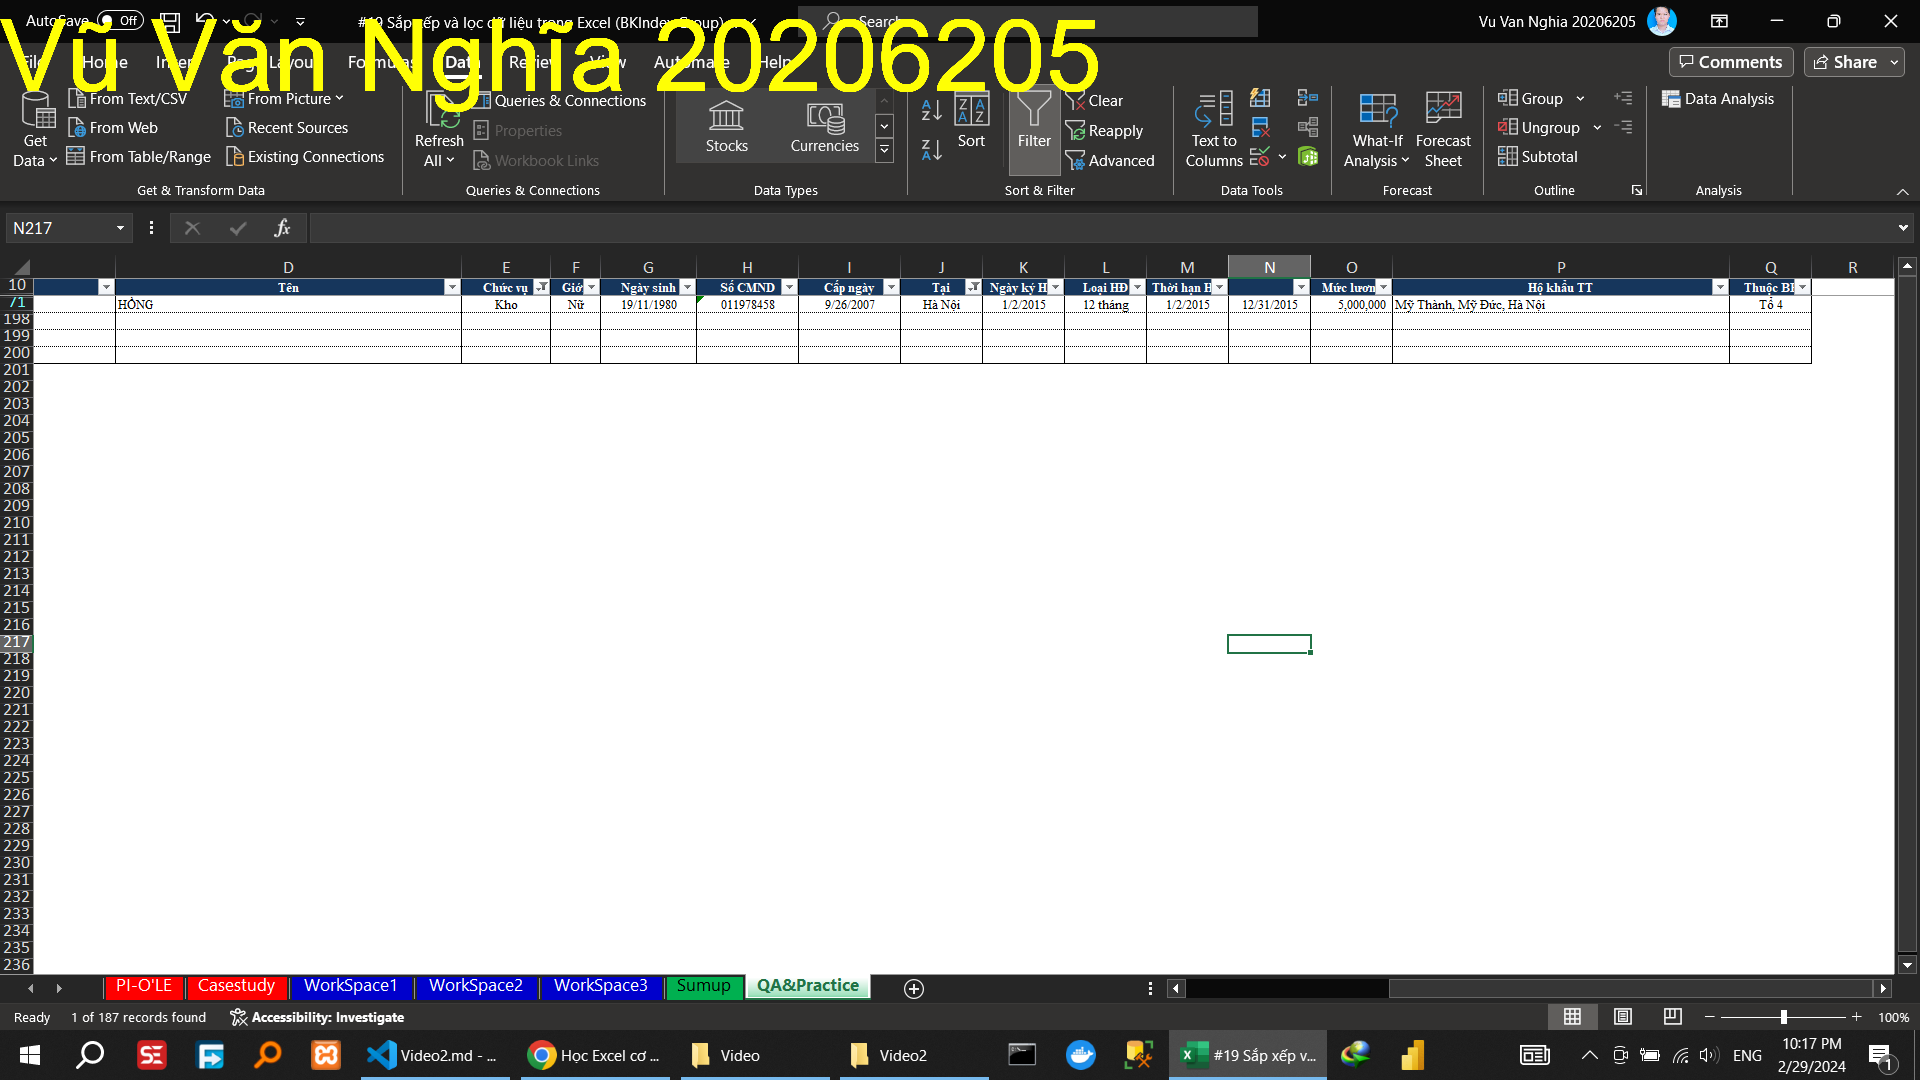
\includegraphics[scale = 0.15]{Video2/ThucHanh/7.png}
%     \caption{Thực hành lọc danh sách nhân viên bộ phận kho có hộ khẩu tại Hà Nội để lên lịch trực tết}
% \end{figure}
% % \newpage
% % \subsection{Video 3}
% % \subsubsection{Hướng dẫn}
% \begin{figure}[h]
%     \centering
%     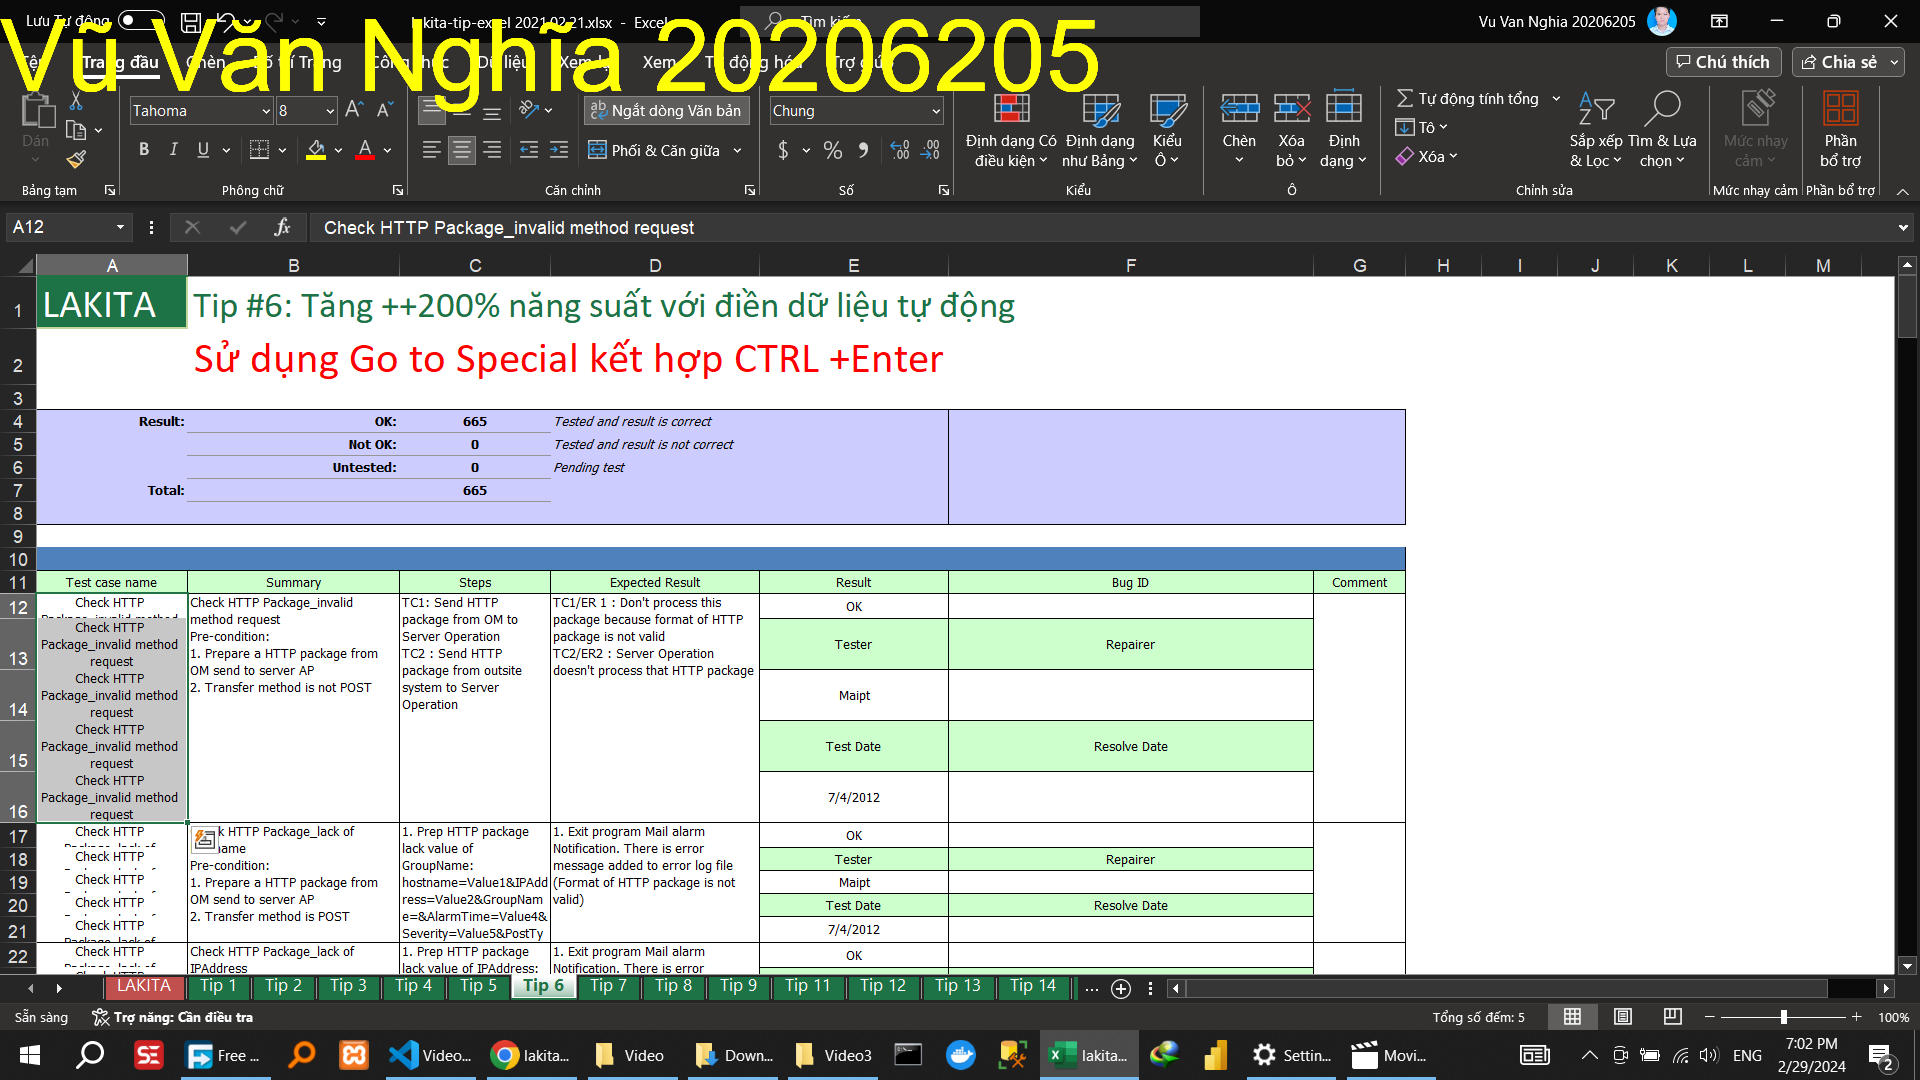
\includegraphics[scale = 0.15]{Video3/HuongDan/1.png}
%     \caption{Hướng dẫn tự động điền thông tin vùng trống}
% \end{figure}
% % \subsubsection{Thực hành}
% % Không có bài tập thực hành
% % \newpage
% % \subsection{Video 4}
% % \subsubsection{Hướng dẫn}

% \begin{figure}[h]
%     \centering
%     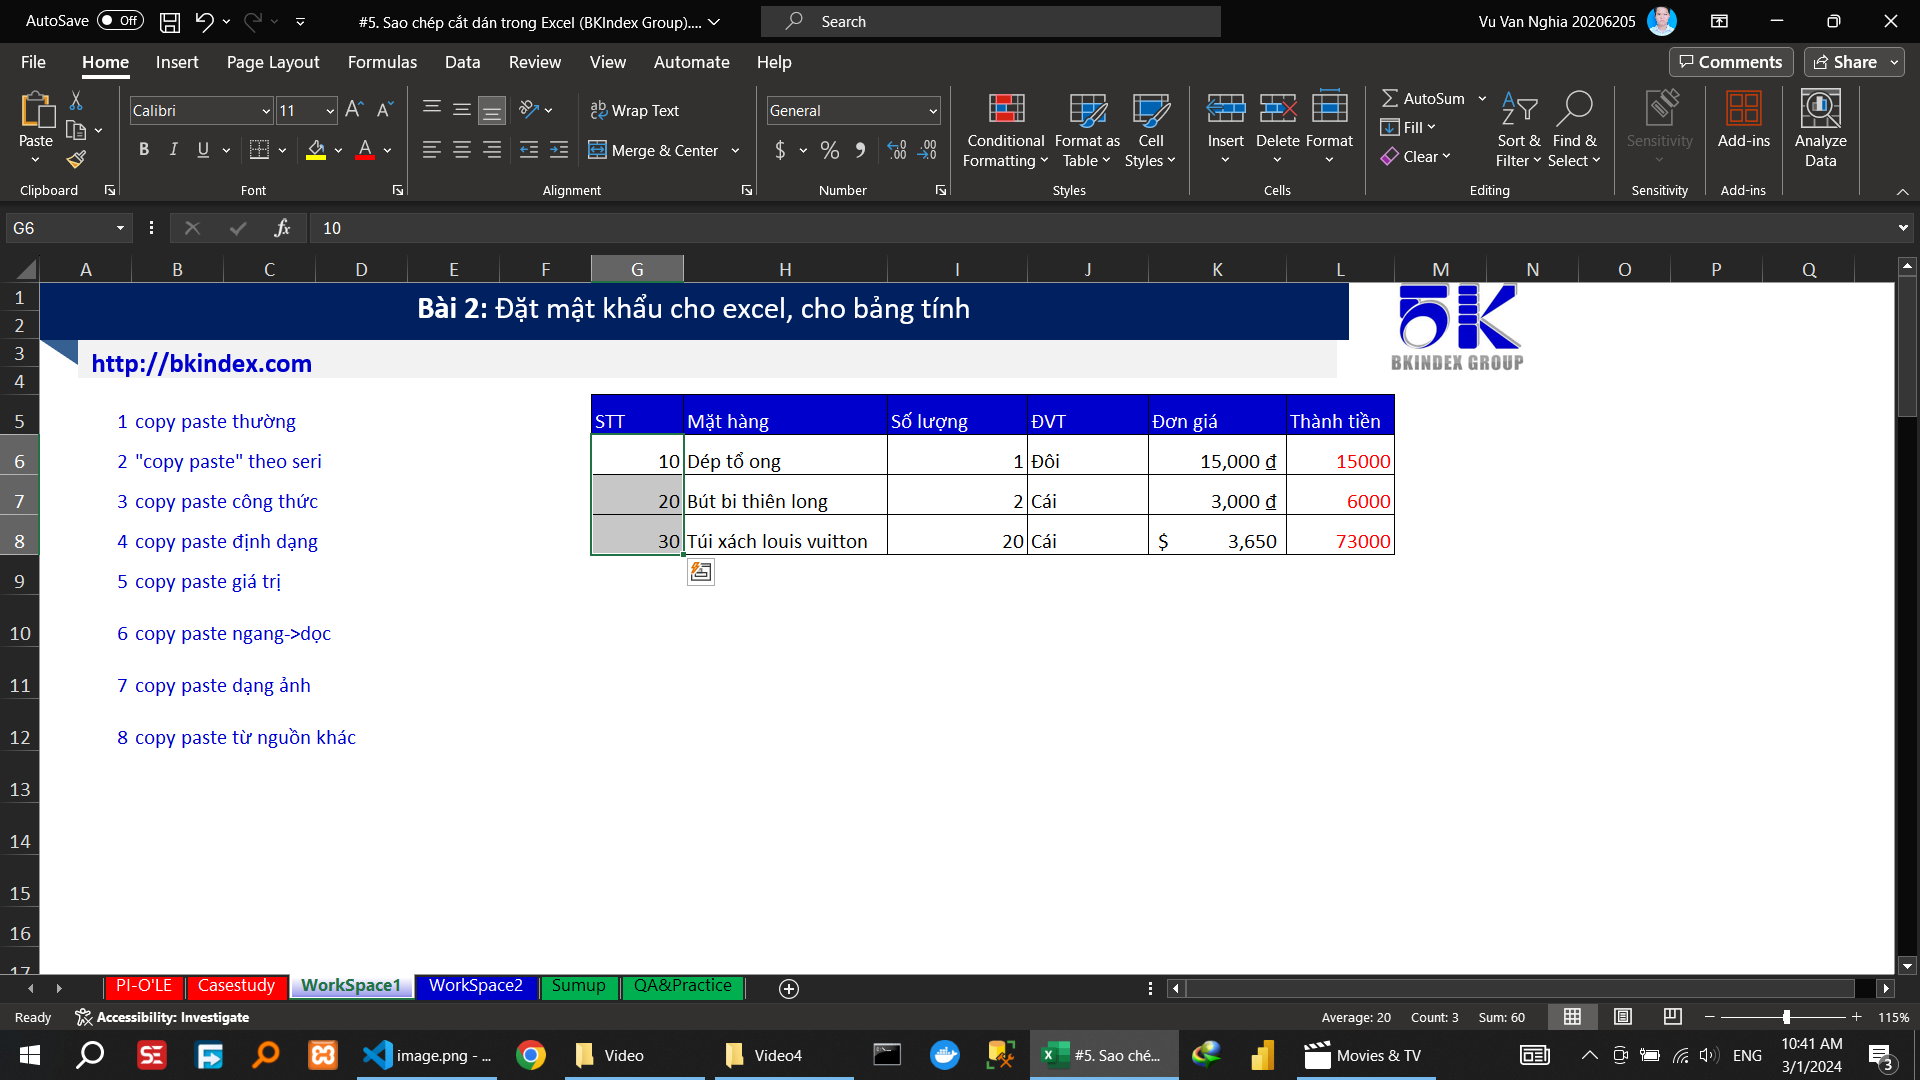
\includegraphics[scale = 0.15]{Video4/HuongDan/1.png}
%     \caption{Hướng dẫn sao chép thông thường cột thành tiền}
% \end{figure}
% \begin{figure}[h]
%     \centering
%     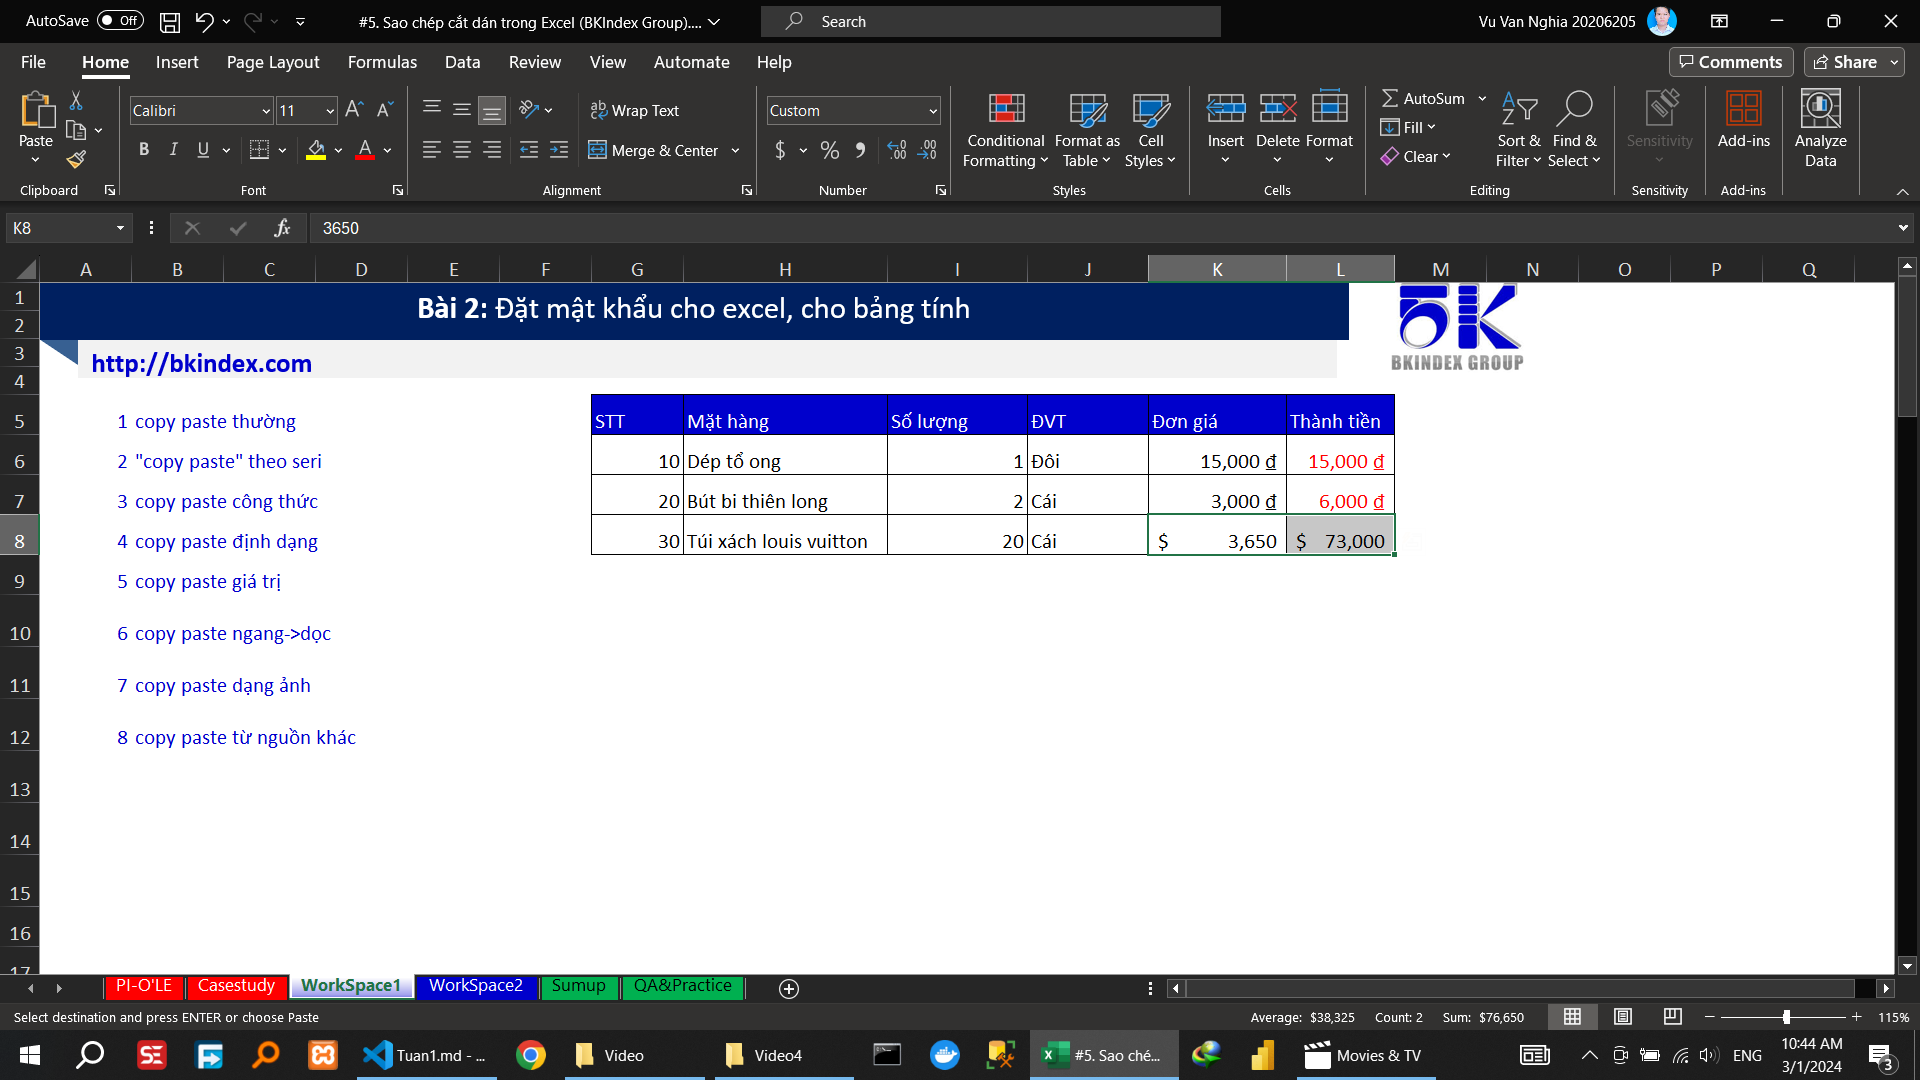
\includegraphics[scale = 0.15]{Video4/HuongDan/2.png}
%     \caption{Hướng dẫn sao chép theo seri số thứ tự}
% \end{figure}







% %? <!-- copy paste công thức		 -->
% %? <!-- copy paste định dạng		 -->
% %? <!-- -->
% %? <!-- copy paste giá trị		 -->
% %? <!-- -->
% %? <!-- copy paste ngang->dọc		 -->
% %? <!-- -->
% %? <!-- copy paste dạng ảnh		 -->
% %? <!-- -->
% %? <!-- copy paste từ nguồn khác		 -->

% %? <!-- Trong video này, Bạn sẽ học Excel với các thao tác:
% %? - Sao chép công thức (copy paste formular excel)
% %? - Sao chép định dạng (copy paste format excel)
% %? - Sao chép giá trị (copy paste value excel)
% %? - Xoay bảng sử dụng sao chép (transpose excel)
% %? - Sao chép dữ liệu bảng thành dạng ảnh (copy paste table as picture)
% %? - Sao chép dữ liệu từ nguồn khác *VD:web) vào Excel (copy from other sources to excel)
% %? - paste special in excel
% %? - copy trong excel
% %? - paste trong excel
% %? - copy and paste in excel
% %? - cách copy trong excel
% %? - paste trong excel chỉ ra định dạng text -->



% % \subsubsection{Thực hành}
% \begin{figure}[h]
%     \centering
%     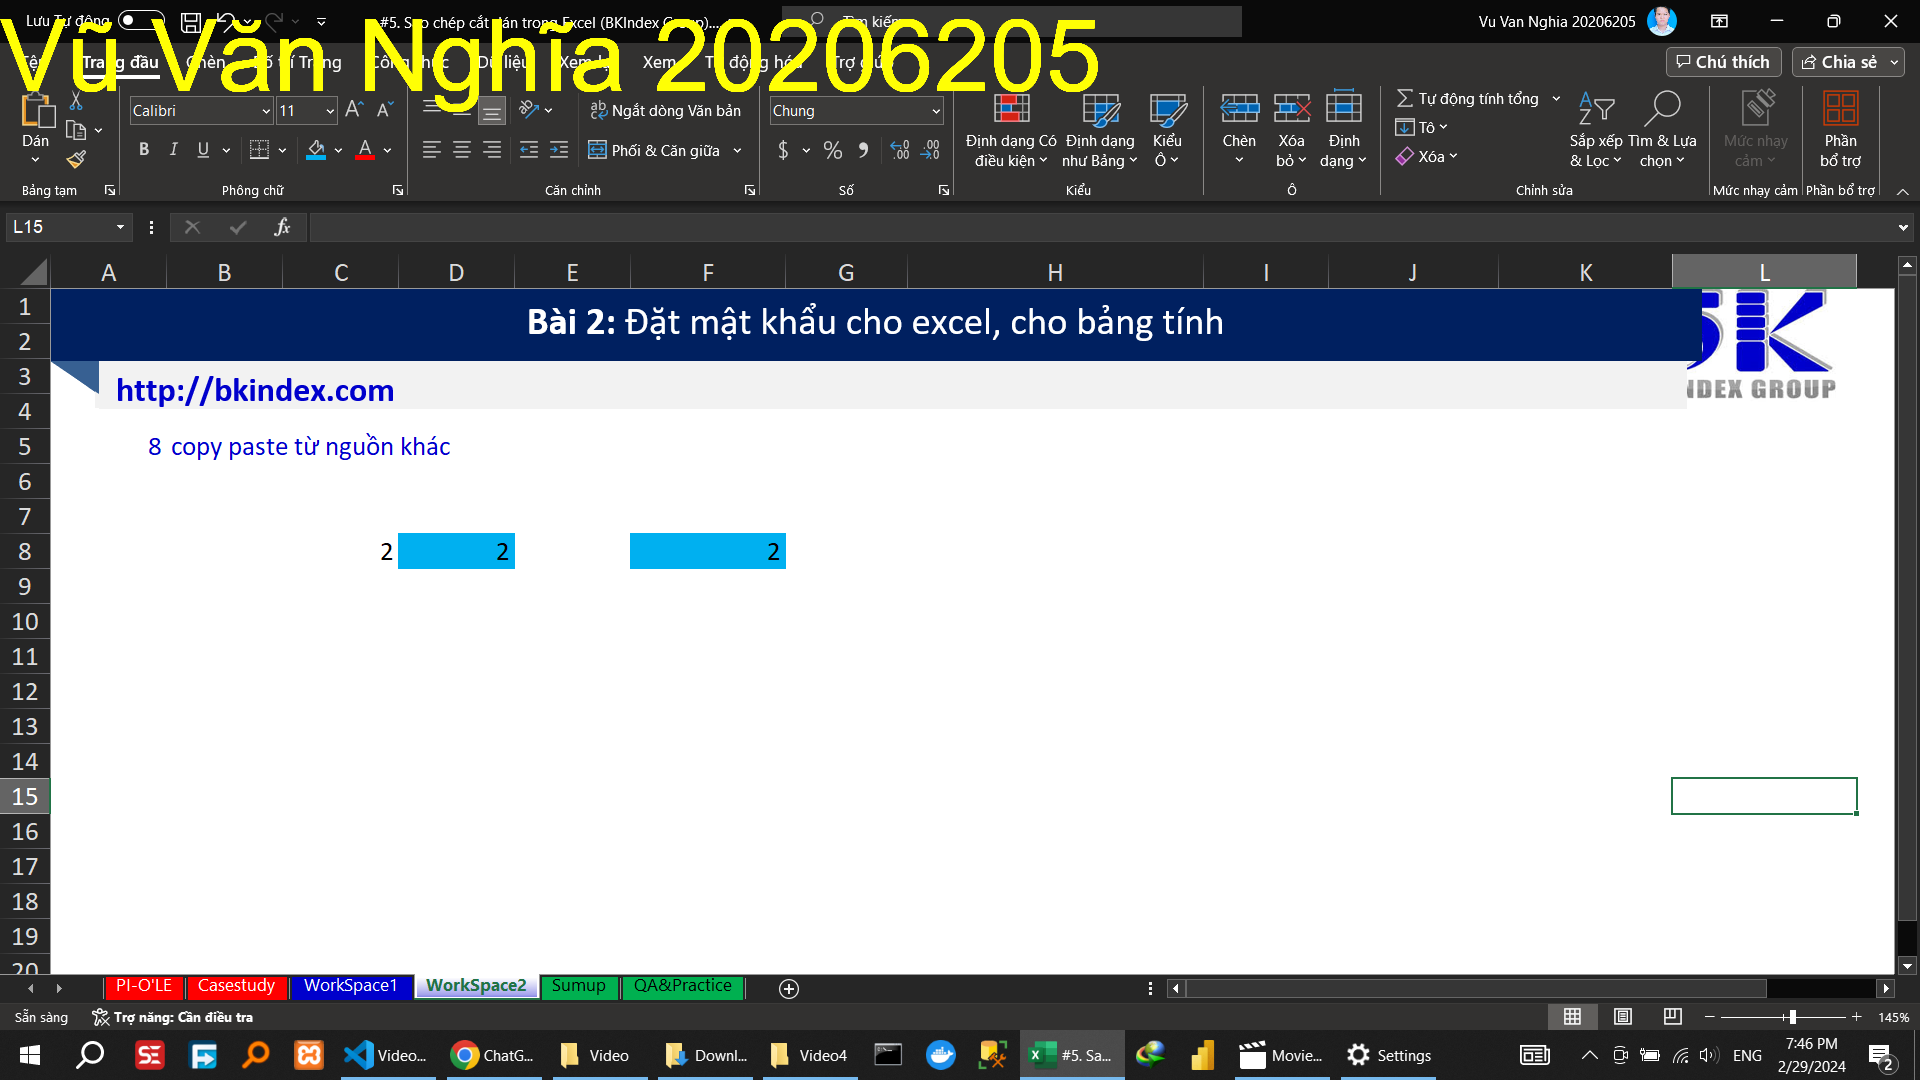
\includegraphics[scale = 0.15]{Video4/ThucHanh/1.png}
%     \caption{Thực hành đổi tên tiêu đề và sao chép giá trị, màu sắc}
% \end{figure}
% % \newpage
% % \subsection{Video 5}
% % \subsubsection{Hướng dẫn}









% % \subsubsection{Thực hành}
% % Không có bài tập thực hành
% % \newpage
% % \subsection{Video 6}
% % \subsubsection{Hướng dẫn}
% % <!-- Trong video này, Bạn sẽ học Excel sử dụng: -->
% % <!-- - Kiểm tra hợp lệ dữ liệu dạng chọn combox (combox data validation excel) -->
% % <!-- - Kiểm tra hợp lệ dữ liệu tùy chỉnh (custom data validation excel) -->
% % <!-- - HIện thông báo khi nhập dữ liệu vào ô kiểm tra dữ liệu (Input message data validation excel) -->
% % <!-- - Hiện thông báo sau khi nhập vào ô kiểm tra dữ liệu (Output message data validation excel) -->
% % <!-- - Sử dụng hàm indirect để làm combox tùy chỉnh (indirect excel) -->
% % <!-- - Data Validation trong Excel -->
% % <!-- - data validation -->
% % <!-- - chuc nang data valdiation trong excel -->
% % <!-- - tạo drop down list -->
% % <!-- - hướng dẫn sử dụng data validation -->
% % <!-- - cach su dung data validation -->
% % <!-- - data validation có chức năng gì -->
% % <!-- - data validation dùng thế nào -->



% % \subsubsection{Thực hành}
% % <!-- Tự học thêm các chức năng -->
% % <!-- Bạn vào chức năng Find&Select và thử các tính năng của nó để dùng cho công việc của mình						 -->
% % Không có bài tập thực hành
% % \newpage
% % \subsection{Video 7}
% % \subsubsection{Hướng dẫn}






% % \subsubsection{Thực hành}
% % Không có bài tập thực hành
% % \newpage
% % \subsection{Video 8}
% % \subsubsection{Hướng dẫn}





% % \subsubsection{Thực hành}

% % '=MOD(ROW(C13),2)=1
% \begin{figure}[h]
%     \centering
%     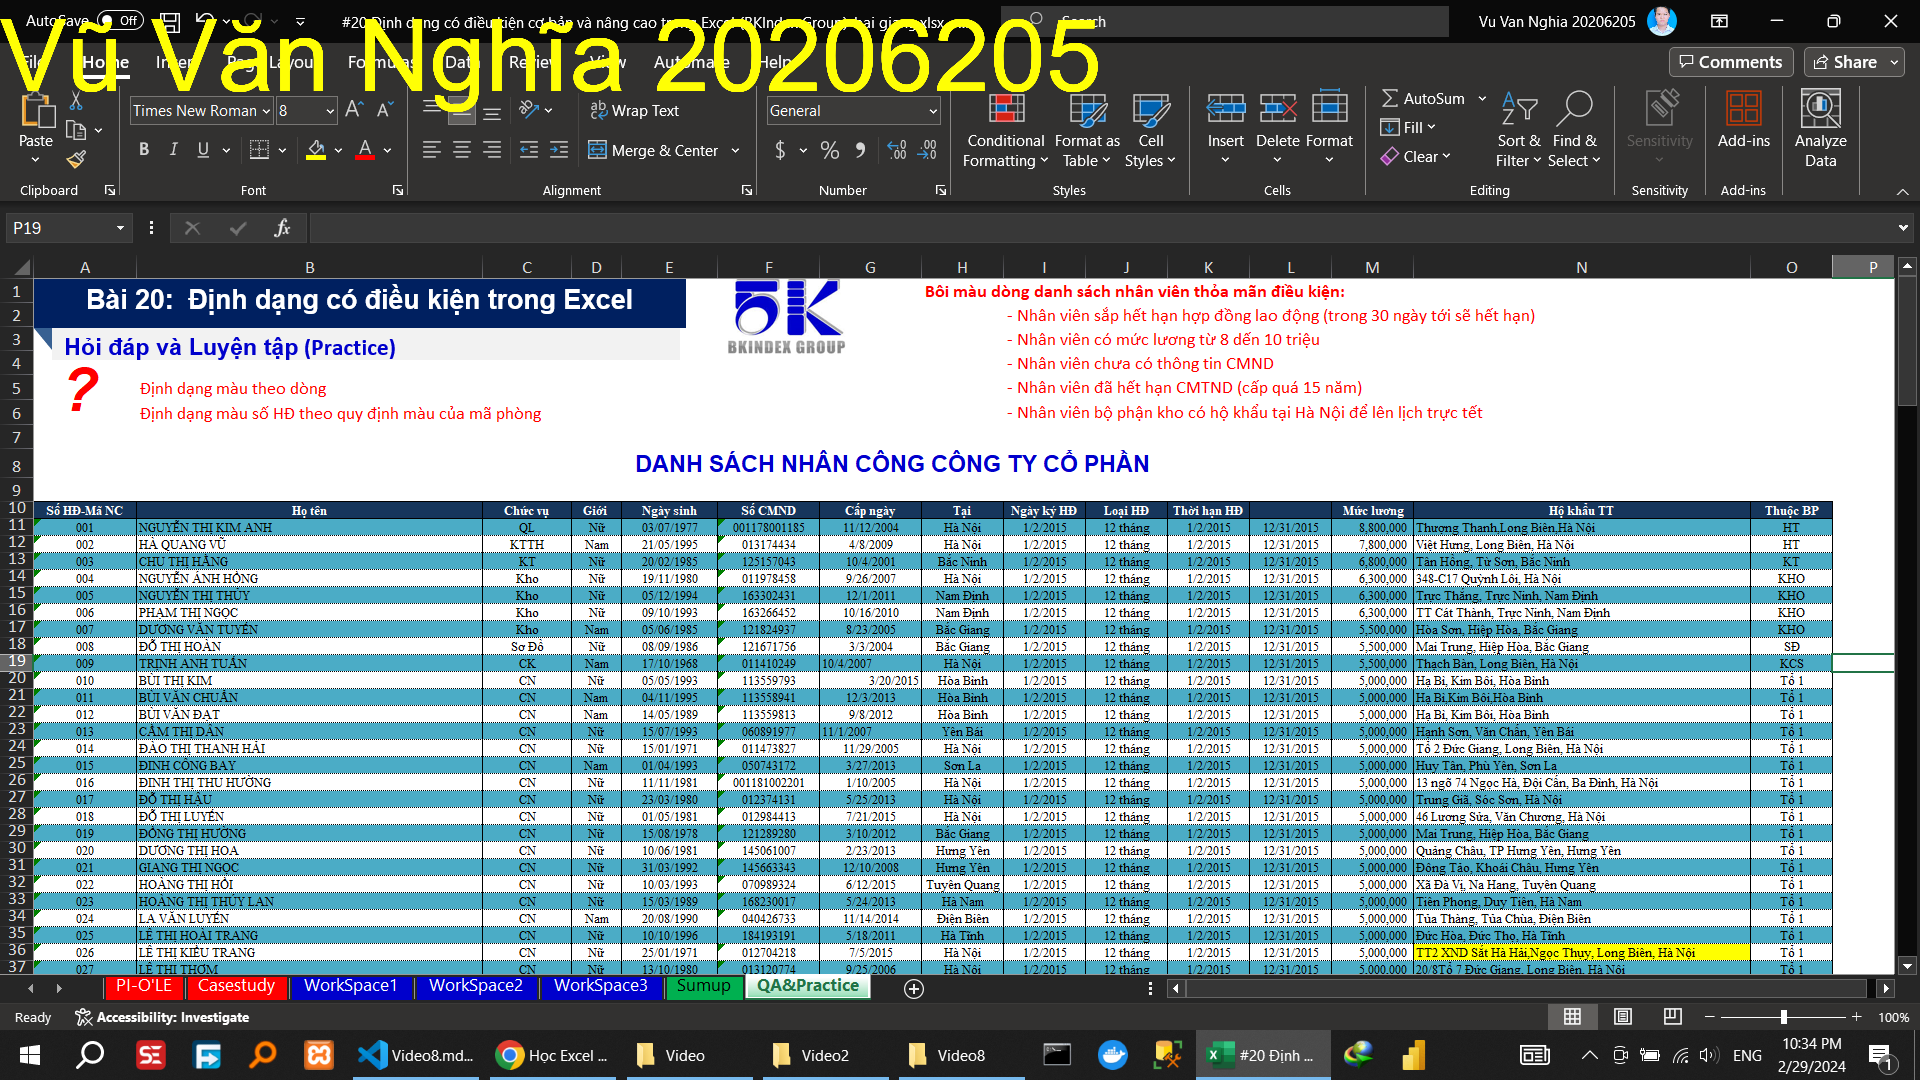
\includegraphics[scale = 0.15]{Video8/ThucHanh/0.png}
%     \caption{Thực hành định dạng màu theo dòng}
% \end{figure}
% \begin{figure}[h]
%     \centering
%     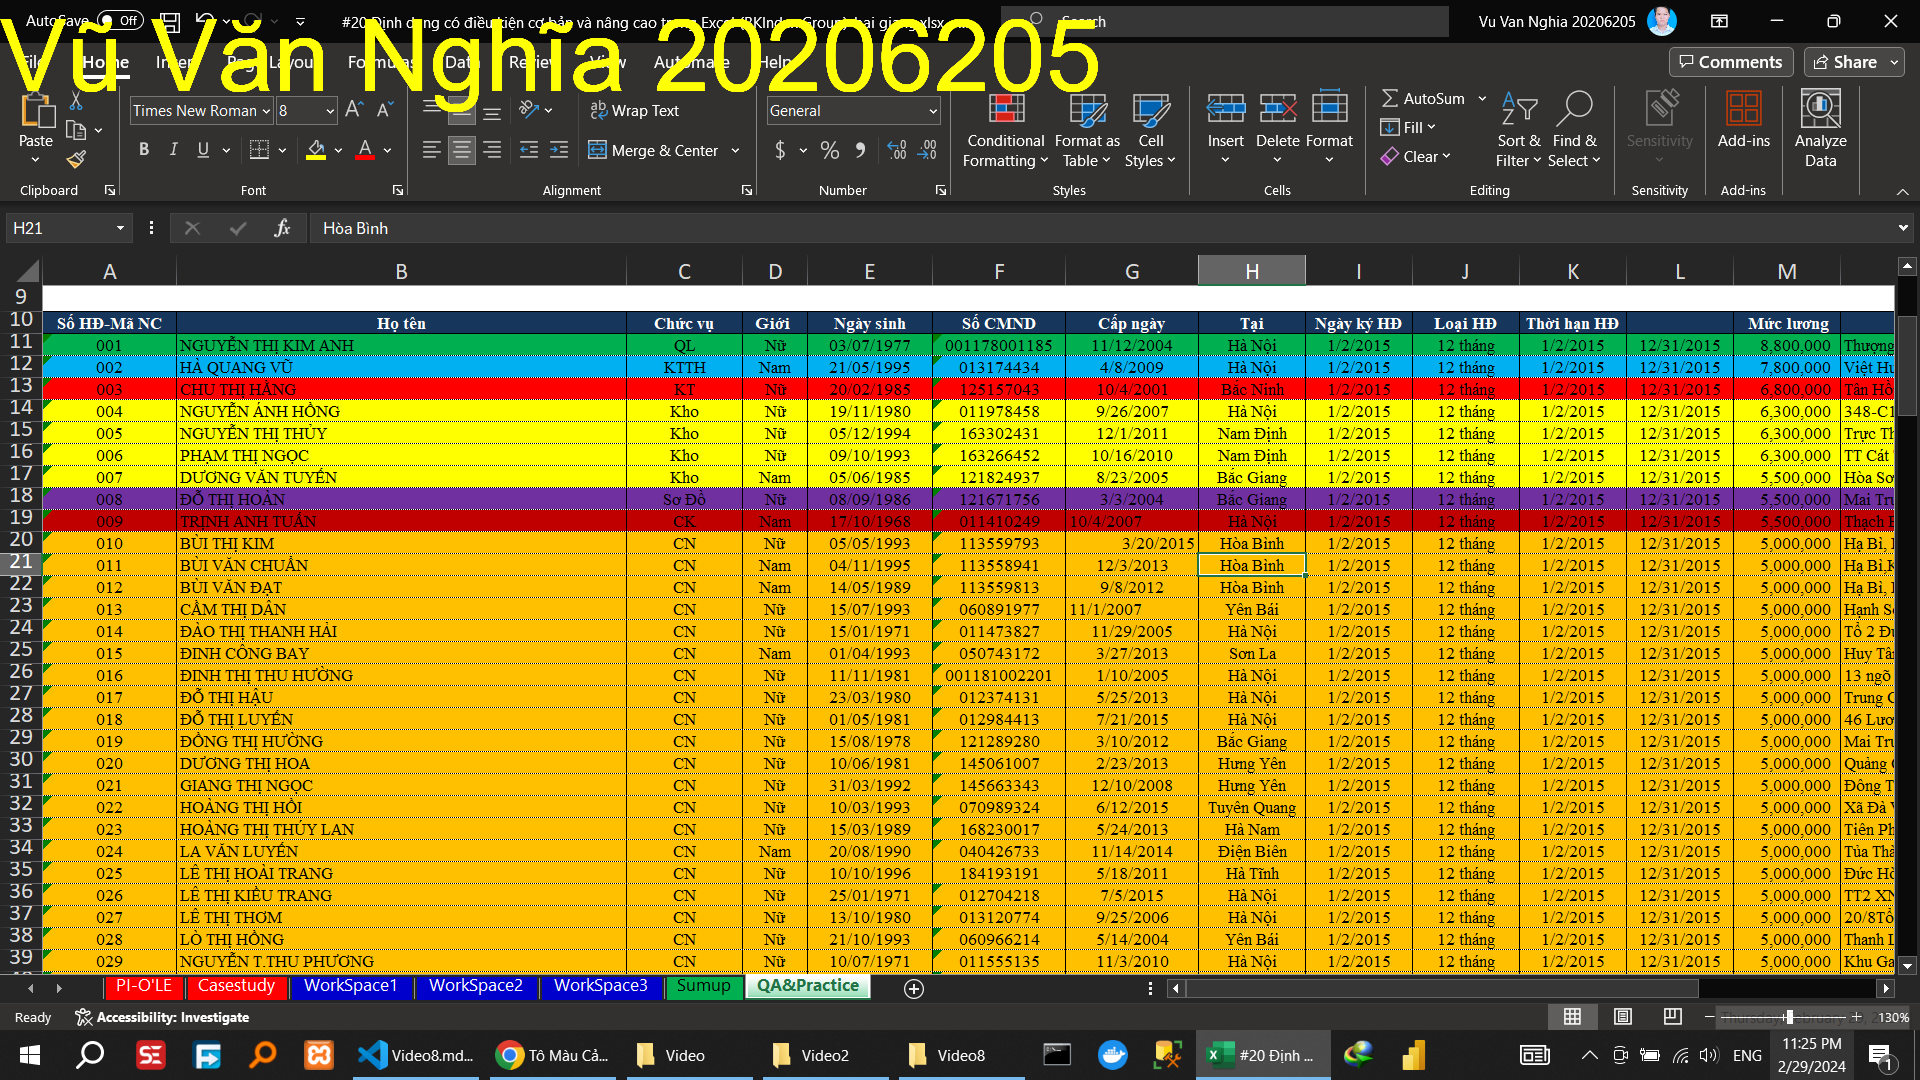
\includegraphics[scale = 0.15]{Video8/ThucHanh/1.png}
%     \caption{Thực hành định dạng màu số HĐ theo quy định màu của mã phòng}
% \end{figure}

% % =$L11-TODAY()<30
% \begin{figure}[h]
%     \centering
%     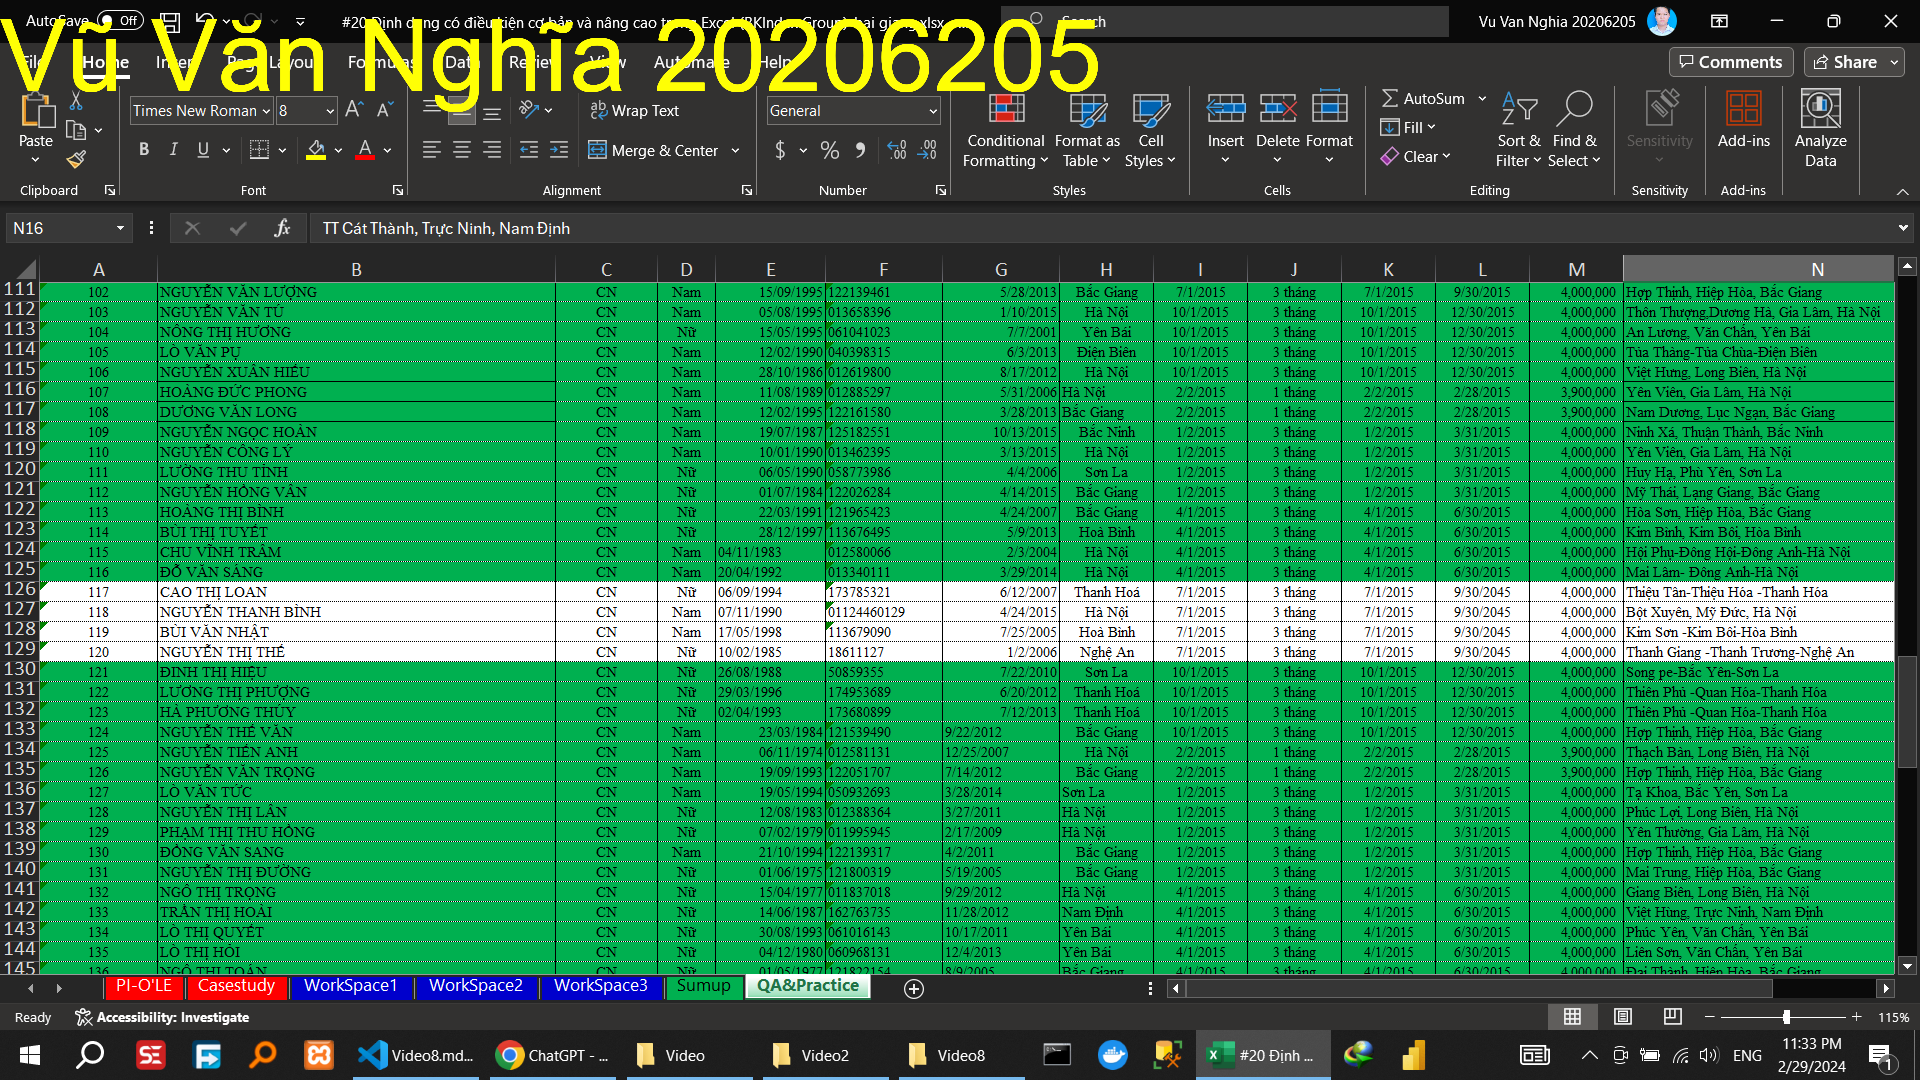
\includegraphics[scale = 0.15]{Video8/ThucHanh/2.png}
%     \caption{Thực hành định dạng màu: Nhân viên sắp hết hạn hợp đồng lao động (trong 30 ngày tới sẽ hết hạn)}
% \end{figure}

% % =AND($M11>=8000000,$M11<=10000000)
% \begin{figure}[h]
%     \centering
%     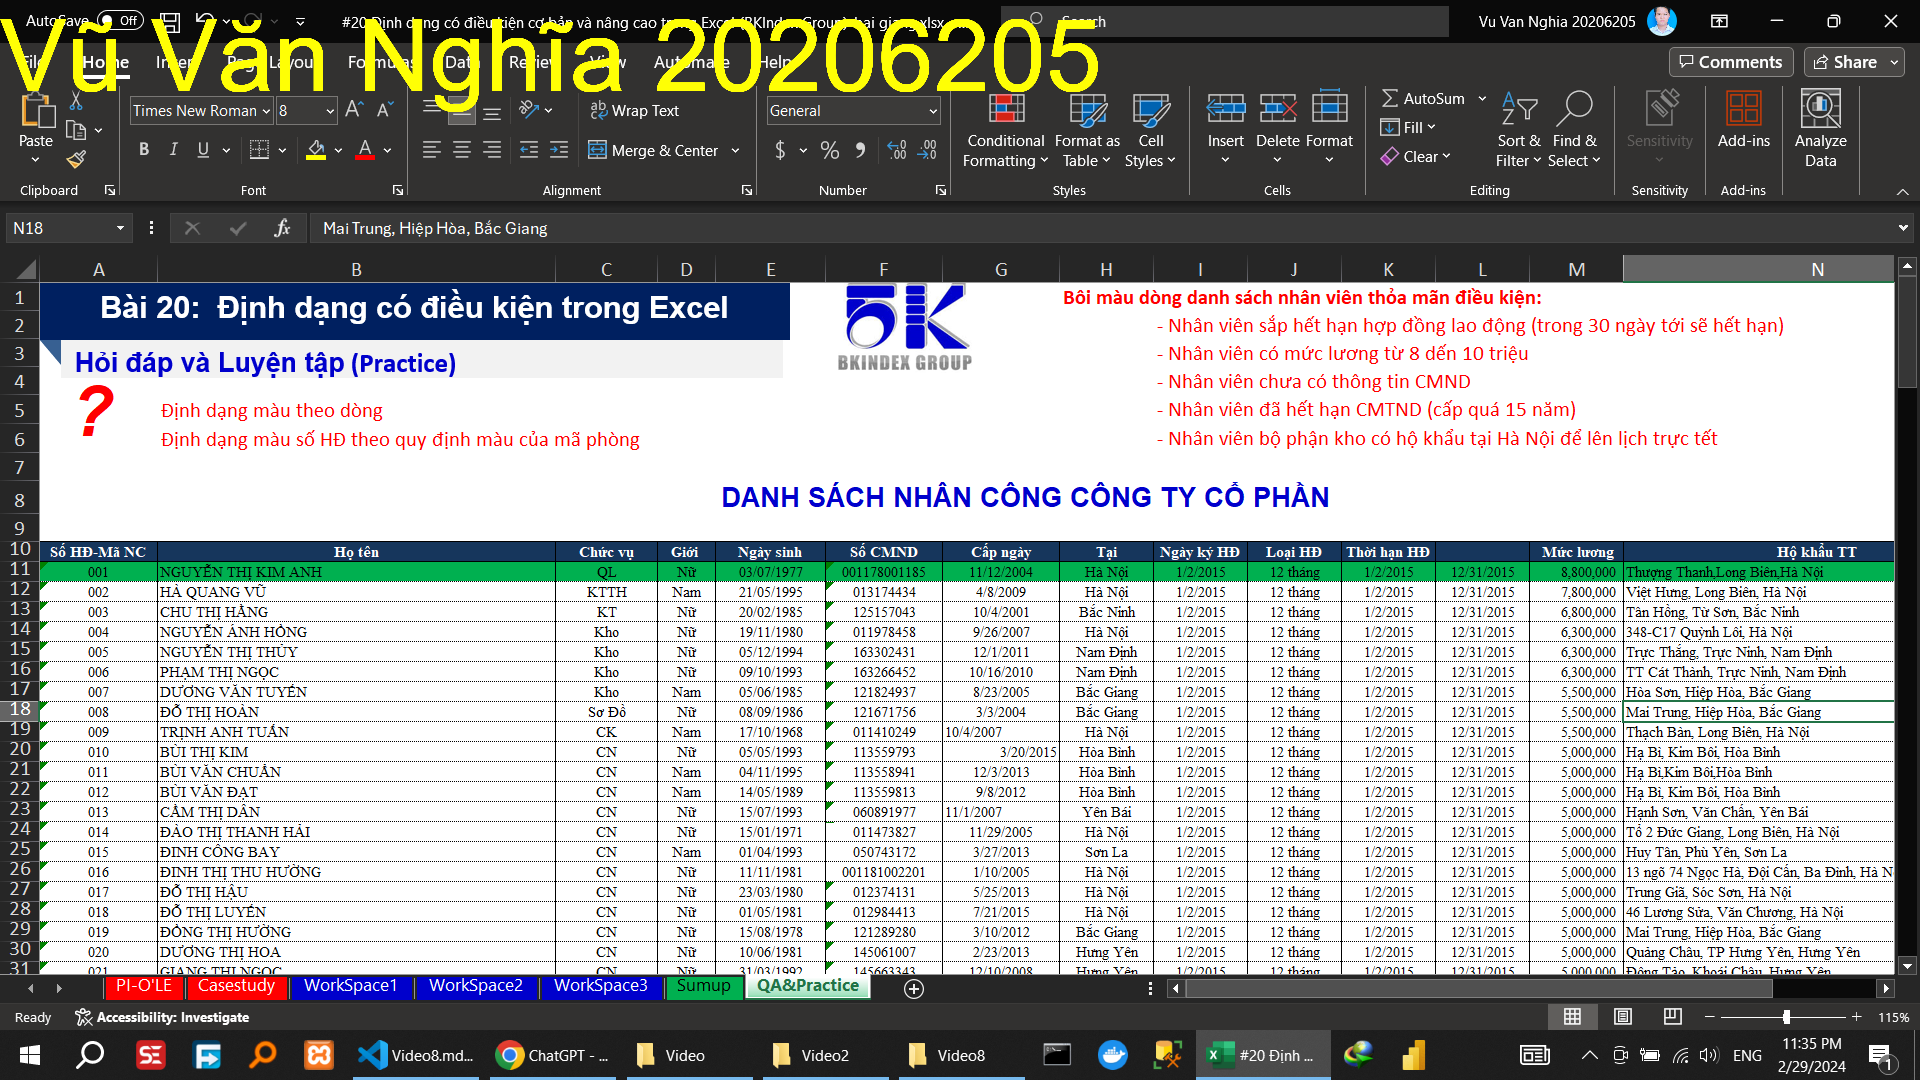
\includegraphics[scale = 0.15]{Video8/ThucHanh/3.png}
%     \caption{Thực hành định dạng màu: Nhân viên có mức lương từ 8 đến 10 triệu}
% \end{figure}

% % =$F11=""
% \begin{figure}[h]
%     \centering
%     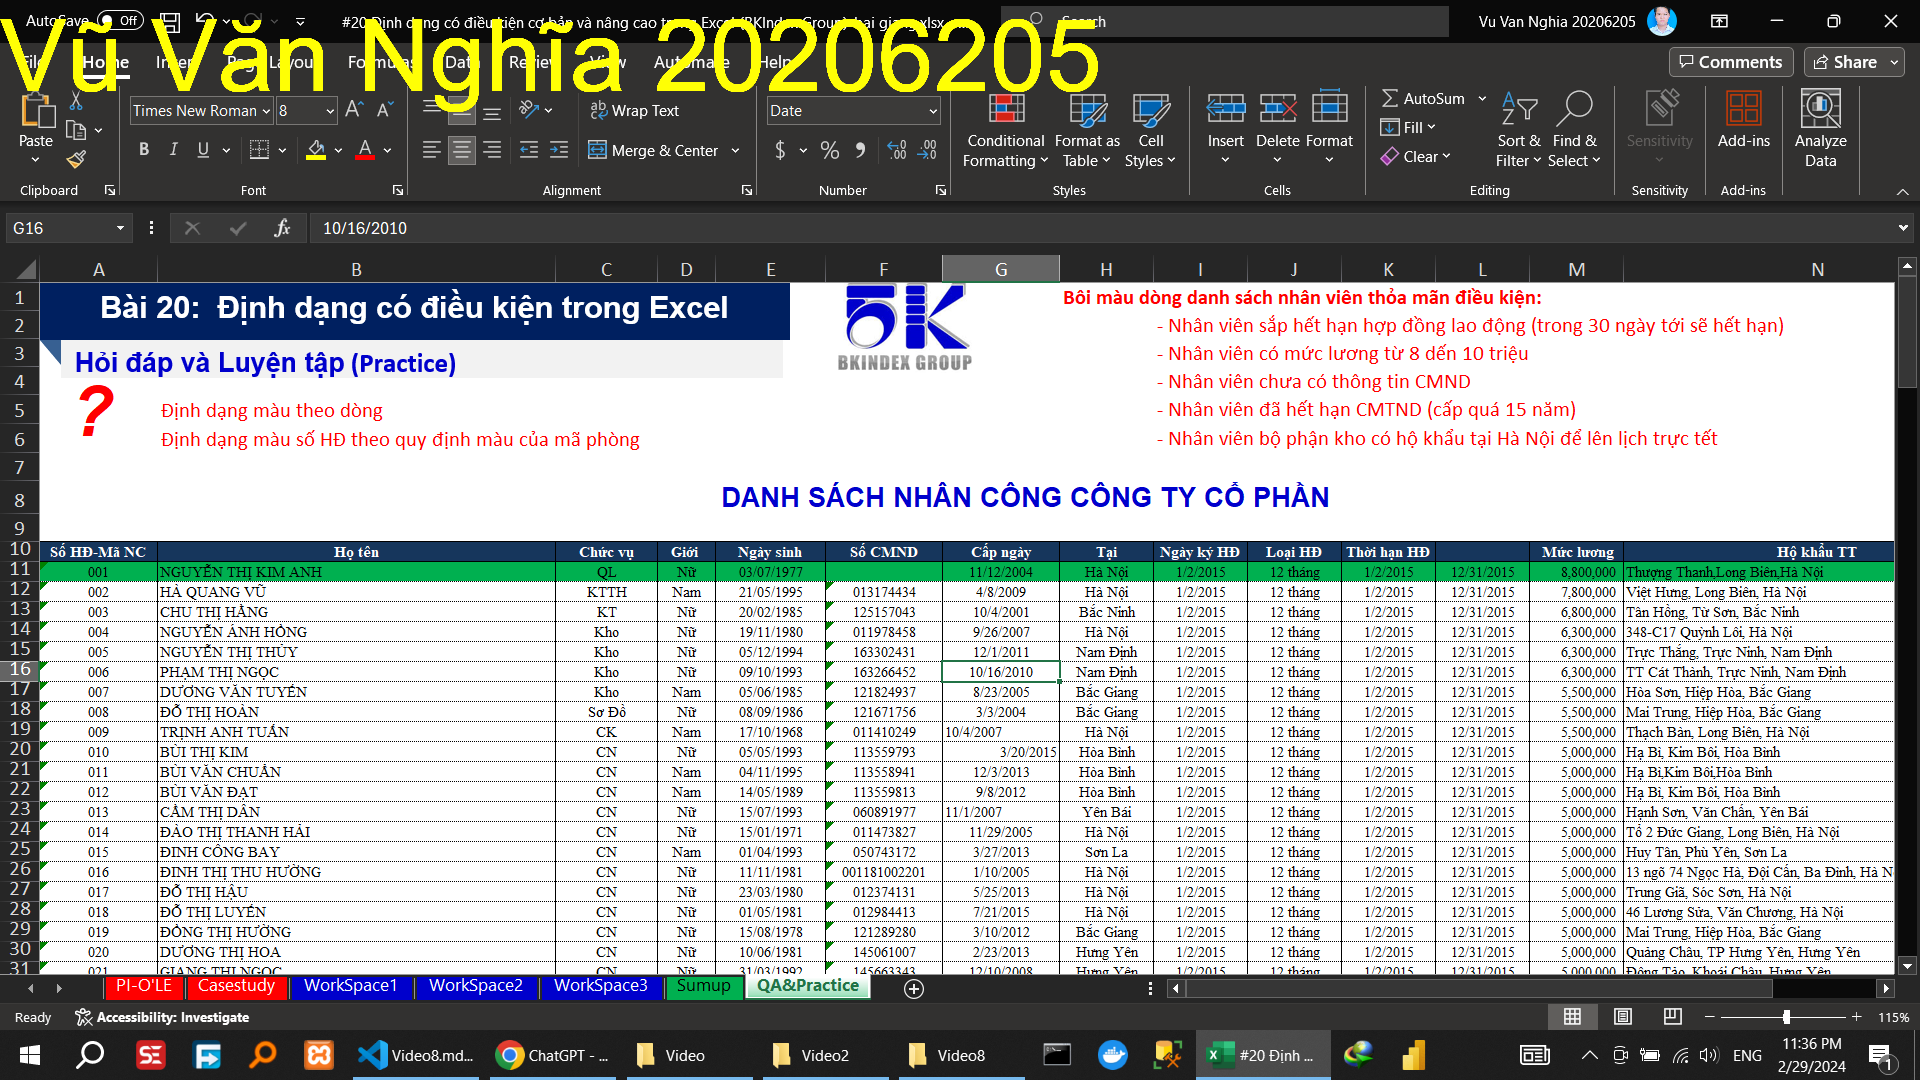
\includegraphics[scale = 0.15]{Video8/ThucHanh/4.png}
%     \caption{Thực hành định dạng màu: Nhân viên chưa có thông tin CMND}
% \end{figure}

% % =DATEDIF($G11, TODAY(), "y") > 15
% \begin{figure}[h]
%     \centering
%     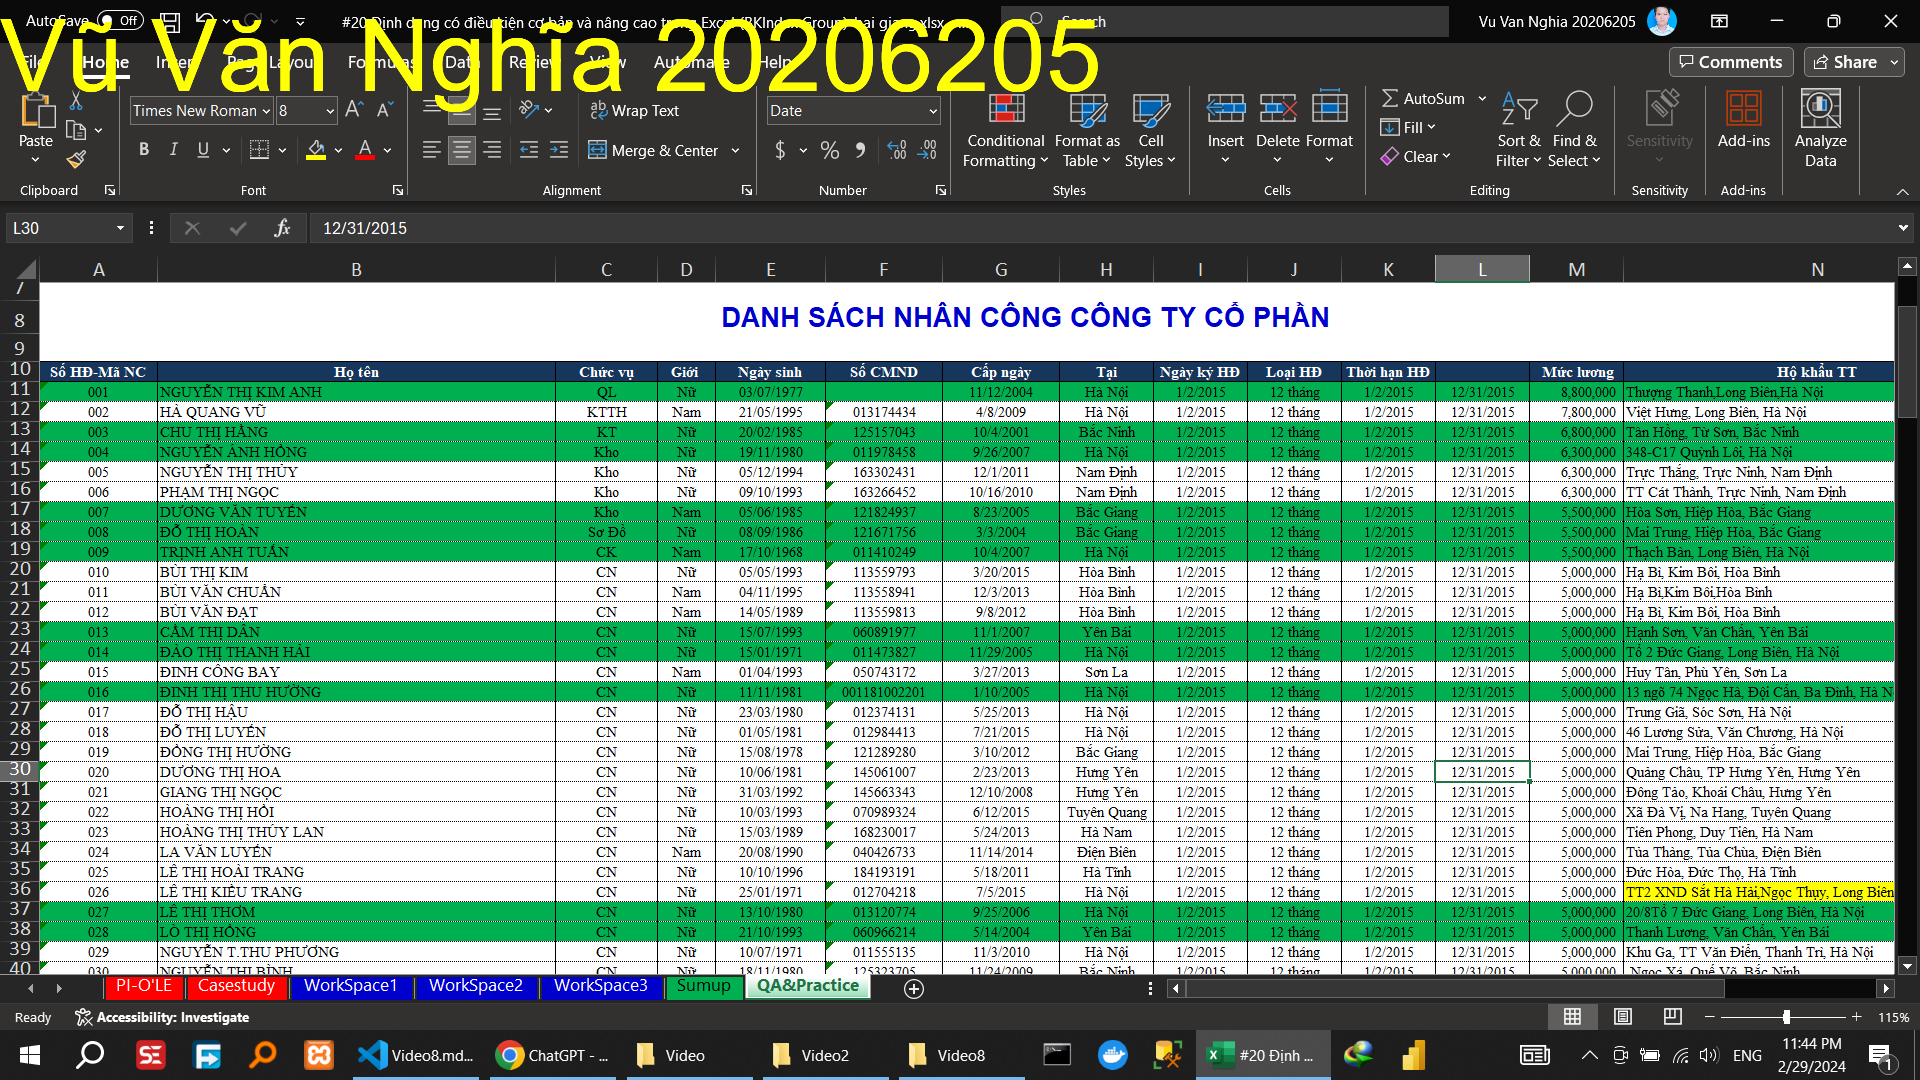
\includegraphics[scale = 0.15]{Video8/ThucHanh/5.png}
%     \caption{Thực hành định dạng màu: Nhân viên đã hết hạn CMTND (cấp quá 15 năm)}
% \end{figure}

% % =AND($C11="Kho", $H11="Hà Nội")
% \begin{figure}[h]
%     \centering
%     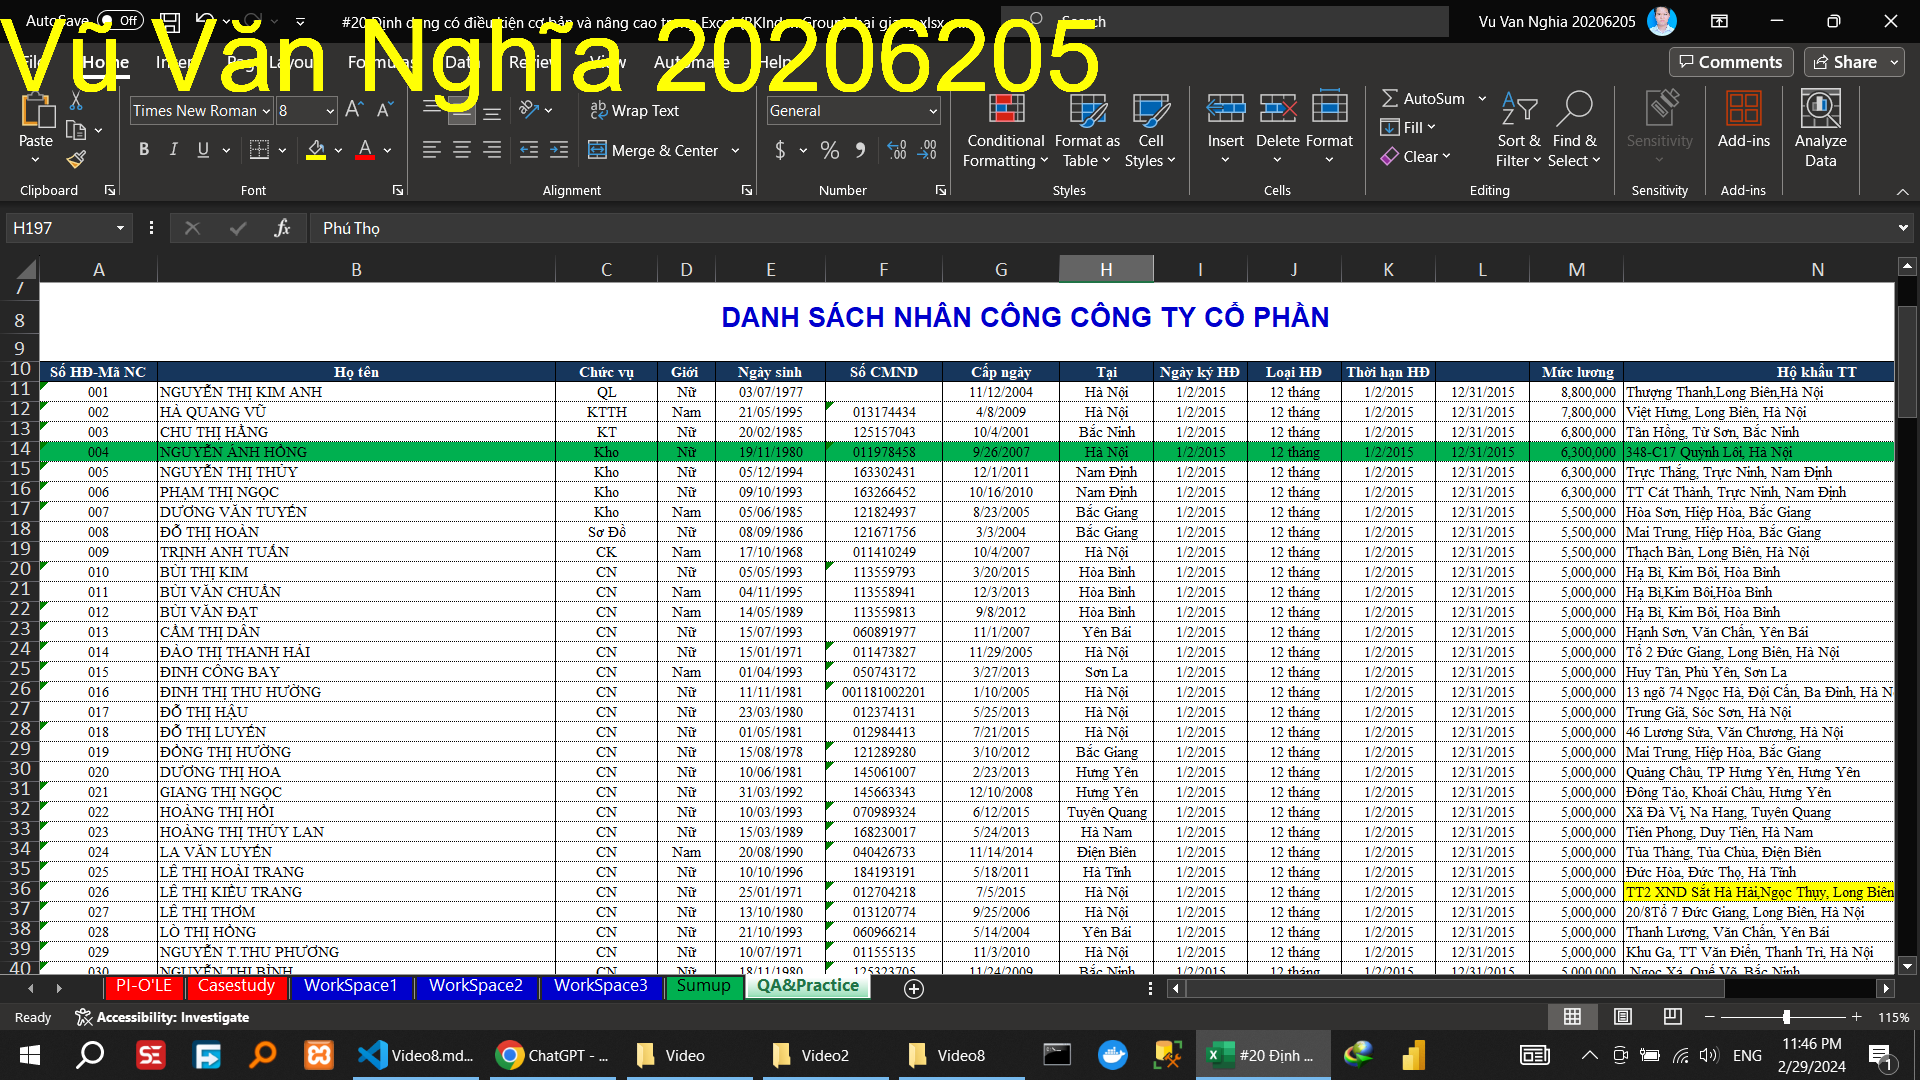
\includegraphics[scale = 0.15]{Video8/ThucHanh/6.png}
%     \caption{Thực hành định dạng màu: Nhân viên bộ phận kho có hộ khẩu tại HN để lên lịch trực tết}
% \end{figure}
%%%%%%%%%%%%%%%%%%%%%%%%%%%%%%%%%%%%%%%%%%%%%%%%%%%%%%%
\end{document}
%%%%%%%%%%%%%%%%%%%%%%%%%%%%%%%%%%%%%%%%%%%%%%%%%%%%%%%
